%%  This is the main file to compile the document
\documentclass[12pt]{article}
\usepackage{setspace}
\usepackage{fullpage} %% better margin use
\usepackage[final]{graphicx}
\usepackage{xcolor,colortbl}
\usepackage{enumitem}
\usepackage{mathtools}
\usepackage{placeins}
%\usepackage{subfig}
\usepackage{caption}
\usepackage{subfigure}
\usepackage{multirow}
\usepackage{amsmath}
\setdescription{leftmargin=\parindent,labelindent=\parindent}
\usepackage{units}
\usepackage{xfrac} %slanted fractions
\usepackage[colorlinks,linkcolor={red},citecolor={red}]{hyperref}
%\hypersetup[colorlinks, linkcolor=red, filecolor=red,  pagecolor=red,
%urlcolor=red]{hyperref}
\usepackage[version=4]{mhchem}
\usepackage{float}

\graphicspath{{./figures/}{./figures/introduction/}{./figures/evaluations/}{./figures/experiment_overview/}{./figures/ratiocalculation/}{./figures/simulation/}{./figures/neutron_energy/}{./figures/energy_shape/}{./figures/isotopics/}{./figures/target_normalization/}{./figures/wraparound/}{./figures/efficiency/}{./figures/uncertainty/}{./figures/validations/}}


\newcommand{\verify}{\textbf{\textcolor{red}{Verify}}}
\newcommand{\etal}{\emph{et al.}}
\newcommand{\ie}{\emph{i.e.}}
\newcommand{\eg}{\emph{e.g.}}
\newcommand{\etc}{\emph{etc}}
\newcommand{\pu}[1][239]{$\mathrm{^{#1}}$Pu}
%\newcommand{\cf}[1][252]{$\mathrm{^{#1}}$Cf} 
\renewcommand{\u}[1][235]{$\mathrm{^{#1}}$U}
\newcommand{\hyd}[1][1]{$\mathrm{^{#1}}$H}  
\newcommand{\talpha}{$\alpha$}
\newcommand{\talphas}{$\alpha$s}
\newcommand{\ftpc}{fissionTPC}
\newcommand{\mev}{MeV}
\newcommand{\mus}{~$\mu$s}
\newcommand{\massunits}{\ensuremath{\mathrm{\mu g /cm^{2}}}}
\renewcommand{\textfraction}{0.15}
\renewcommand{\topfraction}{0.85}
\renewcommand{\bottomfraction}{0.65}
\renewcommand{\floatpagefraction}{0.6}

\newcommand{\HRule}{\rule{\linewidth}{0.5mm}}

%% ==============================================
%%  package for commenting
%%  documentation at: http://get-software.net/macros/latex/contrib/fixme/fixme.pdf
%% ==============================================
% use option 'final' to remove all comments
\usepackage[draft, inline, nomargin]{fixme}
\fxsetup{theme=color, mode=multiuser}
% this create a custom note command for a user
\FXRegisterAuthor{nb}{anb}{\color{blue}NB}      % creates \nbnote{} command
\FXRegisterAuthor{rv}{arv}{\color{red}RV}      % creates \rvnote{} command
 

\bibliographystyle{unsrt}





\begin{document}
%title page
\begin{titlepage}

\begin{center}

% Upper part of the page

\includegraphics[width=0.50\textwidth]{figures/PROSPECT_logo}\\[1cm]    

% Title
\HRule \\[0.4cm]
{\huge \bfseries BiPo Analysis and Plots }
\HRule \\[1.5cm]
\title{BiPo Analysis}

% F.\ Last \\
\emph{\Large Don Jones}\\


\vfill
% Bottom of the page
{\large Last Revision: \today}

\end{center}

\end{titlepage}
\newpage



\section{Plot Description}
\subsection{Description of BiPo events in the AD}
There are two IBD-like "BiPo" backgrounds in the PROSPECT data so termed because they come from decays of bismuth followed by polonium. Because these time-correlated decays are $\beta$-decay followed by $\alpha$-decay they have a topology similar to our IBD events. 
\begin{itemize}
\item{$^{214}\textrm{Bi}\rightarrow^{214}\textrm{Po}\rightarrow^{210}\textrm{Pb}$, the dominant decay seen, and arises from $^{222}$Rn, the ubiquitous radioactive gas from the $^{238}$U decay chain. The half life of $^{222}$Rn is 3.8 days, so a gas-tight detector would see this signal decay away within a few weeks. On the other hand, a detector such as ours is not gas-tight, so we do not expect this BiPo signal to completely disappear. The half-life of $^{214}\textrm{Po}$ is 0.1643(20)~ms giving us a beta followed by an alpha much like the IBD signal. $^{214}\textrm{Bi}$ beta decays 99.98\% of the time with a Q-value of 3.275(15)~MeV. This beta decay only goes to the daughter ground state about 19\% of the time with the remaining 81\% of beta decays having an accompanying gamma ranging in energy from 0.6~MeV to 2.7~MeV (there are a number of decays above this even as high as 3.18~MeV but they occur very rarely). 99.99\% of the time $^{214}$Po alpha decays with a kinetic energy of 7.687~MeV which is quenched to about 0.9~MeV in our detector. }
\item{$^{212}\textrm{Bi}\rightarrow^{212}\textrm{Po}\rightarrow^{208}\textrm{Pb}$ is from the $^{232}$Th decay chain which also has a radon daughter $^{220}$Rn. The half life of $^{220}$Rn is only 56 s, making it much less likely to permeate from external sources. However, given the universal presence of trace radioactive elements like $^{232}$Th, it is not surprising that we would see this decay uniformly throughout our detector. The half-life of $^{212}\textrm{Po}$ is 299(2)~ns. $^{212}\textrm{Bi}$ beta decays 64\% of the time with a Q-value of 2.2515(17)~MeV. This beta decay goes to the daughter ground state about 91\% of the time with the remaining 9\% of beta decays having an accompanying gamma ranging in energy from 0.7~MeV to 1.8~MeV. The  $^{212}\textrm{Po}$ alpha decays 100\% of the time with a kinetic energy of 8.785~MeV which is quenched to about 1.1~MeV in our detector. The short half life of this decay makes it more difficult to measure given that a typical waveform is $\sim$600~ns long, but provides a signal with little accidental background. Due to its short half life, our efficiency for detecting this decay is rather low.}
\end{itemize}

Since these decays are an IBD-like background, they need to be measured and leakage into our IBD selection quantified. In practice, given the high energy resolution of our detector ($<5\%/\sqrt{\textrm{MeV}}$), the alpha peaks from these events are well separated from the neutron capture peak near 0.54~MeV.

In principle, a uniformly dissolved source such as trace $^{232}$Th giving a signature decay sequence can be used to monitor relative cell volumes assuming that rate is proportional to volume. However, our low detection efficiency for the $^{212}$Bi$\rightarrow^{212}$Po decay combined with the already trace amount present in our detector gives a detection rate per cell of less than one decay per hour. A 1\% measure of relative cell volumes with this decay rate would require 1-2 years of data.

This study focuses on using the nearly monoenergetic alphas from these decays to measure the stability of the energy calibration, PSD and the position and energy resolution of the AD. 

\subsection{Plots details}
The following list of plots will be made for both the decays of $^{214}\textrm{Bi}\rightarrow^{214}\textrm{Po}\rightarrow^{210}\textrm{Pb}$ and $^{212}\textrm{Bi}\rightarrow^{212}\textrm{Po}\rightarrow^{208}\textrm{Pb}$.
\begin{enumerate}
\item{Alpha mean energy vs. segment.}
\item{Width (1$\sigma$) of the alpha energy distribution vs. segment.}
\item{Width (1$\sigma$) of the $\Delta$Z distribution, separation distance between the alpha and beta vs. segment. This is a measure of the position resolution and should track the mean of the $\Delta$Z.}
\item{RMS width of the Z-position distribution of alphas vs cell.}
\item{Alpha mean energy versus time ($\sim$24~h bins). Ideally, this should be statistically consistent with a constant.}
\item{Alpha mean energy width versus time ($\sim$24~h bins). This will track detector light yield and transport.}
\item{RMS width of the Z-distribution of alphas averaged across detector versus time. This shows the stability of the position reconstruction over time.}
\item{Width of $\Delta$Z distribution averaged across detector versus time. This tracks the position resolution over time.}
\item{Mean of the Z-position distribution of alphas vs cell. This will be a verification that the position reconstruction is working as expected and should be statistically distributed around zero.}
\item{Alpha energy distribution for whole detector. This will be used to estimate leakage into IBD event selection.}
\item{Beta energy spectrum for whole detector. The shape and endpoint is to be compared with a simulated spectrum to verify that the simulation properly captures the detector performance. }
\item{Whole detector Po alpha Z-position distribution.}
\item{Whole detector $\Delta$Z-position distribution.}
\end{enumerate}
Each plot consists of events that are selected by their time-correlation and as a result, each has an accidental component that must be subtracted. Accidental subtraction is performed using a time offset window. For both alpha decays the offset window starts 10$\times\tau_{214}\approx2.4~ms$ forward from the alpha. The length of the accidentals offset window is set to be 12 times the length of the window for the prompt signal to accumulate more statistics. The accidentals histogram is then scaled by 1/12 to account for this. Other than the timing differences, the signals in the accidentals window are treated exactly the same as those in the prompt window, being subjected to identical cuts and conditions.

\subsection{Message being conveyed by the plots}
The position and energy resolution plots are for monitoring the detector performance and light collection by cell and over time. To a lesser extent these will also be sensitive to wrong calibration values/curves. The energy and Z-width plots will be used to monitor the effectiveness of the calibration to remove time-dependent and segment-to-segment variations. The alpha energy spectra will be used to quantify leakage into the IBD selections and the beta spectrum will be used to benchmark and test simulation.

\section{Data Set}
This section details the data sets included in the plots produced for this document.
\subsection{Production version}
This analysis uses the physics release "Phys\_Neutrino\_v2".
\subsection{Run statistics and information}
A total of 1450.9 hours of data are included from March 5, 2018 to May 30, 2018. The following is a list of the data sets used in these analysis plots. 
%to generate this list run BiPoAnalysis/getRunStats.C
\begin{itemize}
\item{WetCommissioning: 236.086 hours of data between Mon Mar 5, 2018 18:36 and Fri Mar 16, 2018 06:57}
\item{180316\_Background: 286.091 hours of data between Fri Mar 16, 2018 10:51 and Sat Mar 24, 2018 16:53}
\item{180417\_Background: 9.045 hours of data between Tue Apr 17, 2018 23:15 and Wed Apr 18, 2018 08:24}
\item{180420\_Background: 255.938 hours of data between Fri Apr 20, 2018 13:17 and Tue May 1, 2018 10:04}
\item{180501\_ReactorOn: 551.757 hours of data between Tue May 1, 2018 10:07 and Fri May 25, 2018 07:00}
\item{180520\_Background: 111.985 hours of data between Fri May 25, 2018 07:02 and Wed May 30, 2018 00:43}
\end{itemize}
A good runs list was generated for this release and can be found on the Github repository  \href{https://github.com/PROSPECT-collaboration/PROSPECT2x_Analysis/tree/master/Analysis/AnalyzerConfig/Neutrino18_GoodRuns.txt}{here} under the Neutrino\_v2 release. A total of 13 files included in the good runs list failed to be analyzed and were not included. The following is a list of the files that were not included:
\begin{center}
180525\_Background/s000\_f00113\_ts1527659233.root\\ 
180525\_Background/s000\_f00114\_ts1527662848.root\\
180525\_Background/s000\_f00115\_ts1527666470.root\\ 
180525\_Background/s000\_f00116\_ts1527670150.root\\ 
180525\_Background/s000\_f00117\_ts1527673834.root\\
180525\_Background/s000\_f00118\_ts1527677517.root\\ 
180525\_Background/s000\_f00119\_ts1527681255.root\\ 
180525\_Background/s000\_f00120\_ts1527685004.root\\
180525\_Background/s000\_f00121\_ts1527688625.root\\
180525\_Background/s000\_f00122\_ts1527692331.root\\ 
180525\_Background/s000\_f00123\_ts1527695951.root\\ 
180525\_Background/s000\_f00124\_ts1527699567.root\\ 
180525\_Background/s000\_f00125\_ts1527703186.root\\
\end{center}
\subsection{Location of data}
The PhysPulse .h5 files used to make this plot at the time of this writing are stored on wright.physics.yale.edu in the following directory:\\ /projects/prospect/converted\_data/Phys/Phys\_Neutrino\_v2\\ Running the BiPoTreePlugin over these data files will produce a TTree of BiPo events for each run. A copy of these TTrees can be found at the following url:\\ /projects/prospect/converted\_data/Analyzed/Analyzed\_20180601/. \\The name of the TTrees is ``BiPo" and they are found in the BiPoTreePlugin directory of ``AD1\_Wet\_Phys.root" for each run. Analyzed\_20180601 is the same release as Analyzed\_Neutrino\_v2 but was a special pass over the data to produce output specifically including extra plugins including the BiPoTreePlugin which, not included in the first pass.

\section{Event selection and cuts\label{sec:cuts}}
This section deals with the cuts applied to the data to obtain the final event selection. Loose cuts were applied at the plugin-level to limit the size of the event trees. More restrictive cuts were then applied to this event selection in the analysis code that utilized these event trees. The plugin-level cuts were broad enough to include both isotopes of polonium. Some of the more restrictive analysis cuts were isotope-specific.
\subsection{Plugin-level cuts}
The following list of segments were excluded from the analysis inside the BiPoTreePlugin using the ``exclude" feature in the configuration file: 0, 1, 2, 3, 4, 5, 6, 9, 10, 11, 12, 13, 18, 21, 23, 24, 27, 32, 34, 40, 44, 52, 68, 79, 86, 102, 115, 122, 127, 130, and 139. No fiducial cuts were applied to the data either at the cell level or in z-position.
Table \ref{tab:plugincuts} summarizes the cuts made at the plugin level for creating the BiPo event trees.
\begin{table}
\begin{center}
\caption{\label{tab:plugincuts}Event selection cuts applied at the plugin level.}
\begin{tabular}[ht]{c c p{10.5cm}}\hline
Energy and PSD&~&~\\\hline\hline
Alpha energy &\vline& $0.72~\textrm{MeV}<$E$_{\alpha}<1.27~\textrm{MeV}$\\
Alpha PSD cut& \vline&$0.18<$PSD$_{\alpha}<0.34$\\
beta cluster energy &\vline& $\leq 5$~MeV\\
beta energy & \vline&Cluster discarded unless all events in it are $\leq 4$~MeV\\
beta PID & \vline&PID==CLUSTER\_IONI (P2X cluster classification which excludes clusters with events in the recoil PSD band)\\
beta PSD & \vline&$0<$PSD$_{\beta}<0.3$\\\hline
Spatial topology&~&~\\\hline\hline
$x/y$ (cell) cut &\vline& No cut on prompt/delayed relative cell positions\\
$z$-position&\vline& No cut on absolute $z$-position except $z\neq \pm1000$~mm\\
$\Delta z$&\vline&Difference in position between delayed alpha and first beta candidate in cluster $<20$~cm\\\hline
Timing&~&~\\\hline\hline
$\Delta t=t_{\alpha}-t_{\beta}$&\vline &$0< dt < 3\tau$, where $\tau$ is the lifetime of Po-214 given by $0.1643/\ln{(2)}~$ms\\\hline

\end{tabular}
\end{center}
\end{table}
\subsection{Analysis-level cuts}
More restrictive cuts were applied in the analysis code running over these event trees, some of which were dependent upon the polonium isotope being plotted.
Although the code is set up to handle fiducial cuts, neither $z$ nor cell-wise fiducial cuts were applied in this analysis. Table \ref{tab:analysiscuts} summarizes the cuts applied at the analysis level.
\begin{table}
\begin{center}
\caption{\label{tab:analysiscuts}Event selection cuts applied in the analysis code. Cuts that are isotope-specific are specified by ``214" for $^{214}$Po and ``212" for $^{212}$Po.}
\begin{tabular}[ht]{c c p{10.5cm}}\hline
Energy and PSD&~&~\\\hline\hline
Alpha energy &\vline& $0.75~\textrm{MeV}<$E$_{\alpha}(214)<1.00~\textrm{MeV}$\\
~&\vline&$0.97~\textrm{MeV}<$E$_{\alpha}(212)<1.26~\textrm{MeV}$  \\
Alpha PSD cut& \vline&$0.18<$PSD$_{\alpha}<0.34$\\
beta cluster energy &\vline& E$_{tot}\leq 4$~MeV\\
beta PSD & \vline&First event in prompt cluster $0<$PSD$_{\beta}<0.26$\\\hline
Spatial topology&~&~\\\hline\hline
$x/y$ (cell) cut &\vline& No cut on prompt/delayed relative cell positions\\
$z$-position&\vline& No cut on absolute $z$-position except $z\neq \pm1000$~mm\\
$\Delta z$&\vline&Difference in position between delayed alpha and first beta candidate in cluster $<20$~cm\\\hline
Timing&~&~\\\hline\hline
$\Delta t=t_{\alpha}-t_{\beta}$&\vline &$10~\mu\textrm{s}< \Delta t(214) < 3\tau$, where $\tau$ is the lifetime of Po-214 \\
~&\vline&$0.2~\mu\textrm{s}< \Delta t(212) < 6~\mu$s\\\hline

\end{tabular}
\end{center}
\end{table}

Figures \ref{fig:apsd212} and \ref{fig:apsd214} show the PSD selection for the delayed alphas. The full energy range covering the alphas in both decay chains is included.
It is worth noting that only the PSD, position and energy of the first event in the prompt cluster is recorded. Therefore, further cuts on these quantities on the prompt beta are limited to the first event in the prompt cluster. In addition to the parameters of the first event, the displacement of the prompt event furthest away from the delayed alpha is also saved as the ``max\_dist" variable. There was no obvious place to cut on this variable so no cut on ``max\_dist" was applied. Figures \ref{fig:bpsd212} and \ref{fig:bpsd214}show the PSD and energy selection for the prompt betas. 

The half-life of the $^{214}$Po decay is 0.1643~ms. The time difference between the prompt beta and delayed alpha candidates for this decay is limited to 0.01~ms$<$dt$<3\times\tau$ where $\tau=0.1643/ln(2)$~ms, the lifetime of $^{214}$Po. Figure \ref{fig:dt214} show2 the $\Delta$t distribution. A fit to the half-life of $^{214}$Po is in good agreement with the accepted value.

The half-life of the $^{212}$Po decay is 299~ns. The time difference between the prompt beta and delayed alpha candidates for this decay is limited to 200~ns$<$dt$<6~mu$s. The time distribution (see Figure \ref{fig:dt212}) below 650~ns is shaped by artifacts of the length of the waveforms and an analysis hold off time.  A fit to the half-life of $^{212}$Po is in good agreement with the accepted value. Only the data from 660~ns upward is used in the half-life fit. However, the result of the fit is extended (dashed line) over the whole data set to justify the use of data outside this region. The entire data set from 0 to 6~$\mu$s is used in this analysis. 

Accidental subtraction is performed using a time offset window. For both alpha decays the offset window starts 10$\times\tau_{214}\approx2.4~ms$ forward from the alpha. The length of the accidentals offset window is set to be 12 times the length of the window for the prompt signal to accumulate more statistics. The accidentals histogram is then scaled by 1/12 to account for this. Other than the timing differences, the signals in the accidentals window are treated exactly the same as those in the prompt window, being subjected to exactly the same cuts and conditions.

The maximum displacement between the delayed alpha and any event in the prompt cluster, ``max\_dist", was also calculated and stored in the TTrees. However, there was no obvious place to cut on this value so no cut was applied. 

A broad multiplicity cut was applied in the BiPoTreePlugin to limit clusters to multiplicity less than 20, meaning that clusters with more than 20 hits were rejected.

\section{Software}
These plots were produced in a two step sequence. First, a TTree of BiPo candidates was produced for each run using the plugin framework from P2X. The plugin is called BiPoTreePlugin which lives in the PhysPulse directory. PhysPulse plugins operate on calibrated data, that is, data where pulse energy is calibrated to remove position dependence and where timing offsets due to hardware configurations and cable lengths have been removed. The cuts applied at the plugin level are relatively loose to allow for studies with restricting cuts later. Second, two programs are called to run over the BiPo TTrees and make the plots. The plots of variables such as energy and resolution versus time are made using the program ``BiPovsTime.C". The remaining plots that are averages over all time are made using ``BiPoPlotter.C".  Both of these ROOT macros use the same set of cuts on the data. See Sec. \ref{sec:cuts} for information on the cuts applied. For information on obtaining or viewing this code from the Github see Sec. \ref{sec:github} 
\subsection{Code used to generate plots}
The code required to do this analysis is all available on the Github (see Sec \ref{sec:github}). Production of the BiPo TTrees requires a working version of P2X. 
To build the BiPo TTrees run the script runBiPoTTreePlugin.sh
To plot results run BiPovsTime.C and BiPoPlotter.C from inside a ROOT terminal. 
\subsection{Github repository information\label{sec:github}}
The repository for P2X which includes the BiPoTree plugin can be cloned at\\ https://github.com/PROSPECT-collaboration/PROSPECT2x\_Analysis.git\\
The commit used in this analysis is \\
commit 49798e8b6196c75114eb7fdd658429fc35dbd57f\\
Date:   Thu May 31 22:56:59 2018 -0400\\

The Github repository containing the analysis code includes a README file with instructions for reproducing these plots. The repository can be cloned at \\
https://github.com/jonesdc76/BiPoAnalysis\\
The commit used to make these plots is\\
commit a78beff90c58e8e4cfb8b1aa5f9493078a11e05f\\
Date:   Thu Jun 7 14:50:17 2018 -0400
\newpage
%------------------------------
\section{Plots of interest}
\subsection{Energy versus segment plots}
\begin{figure}[!h]
\centering
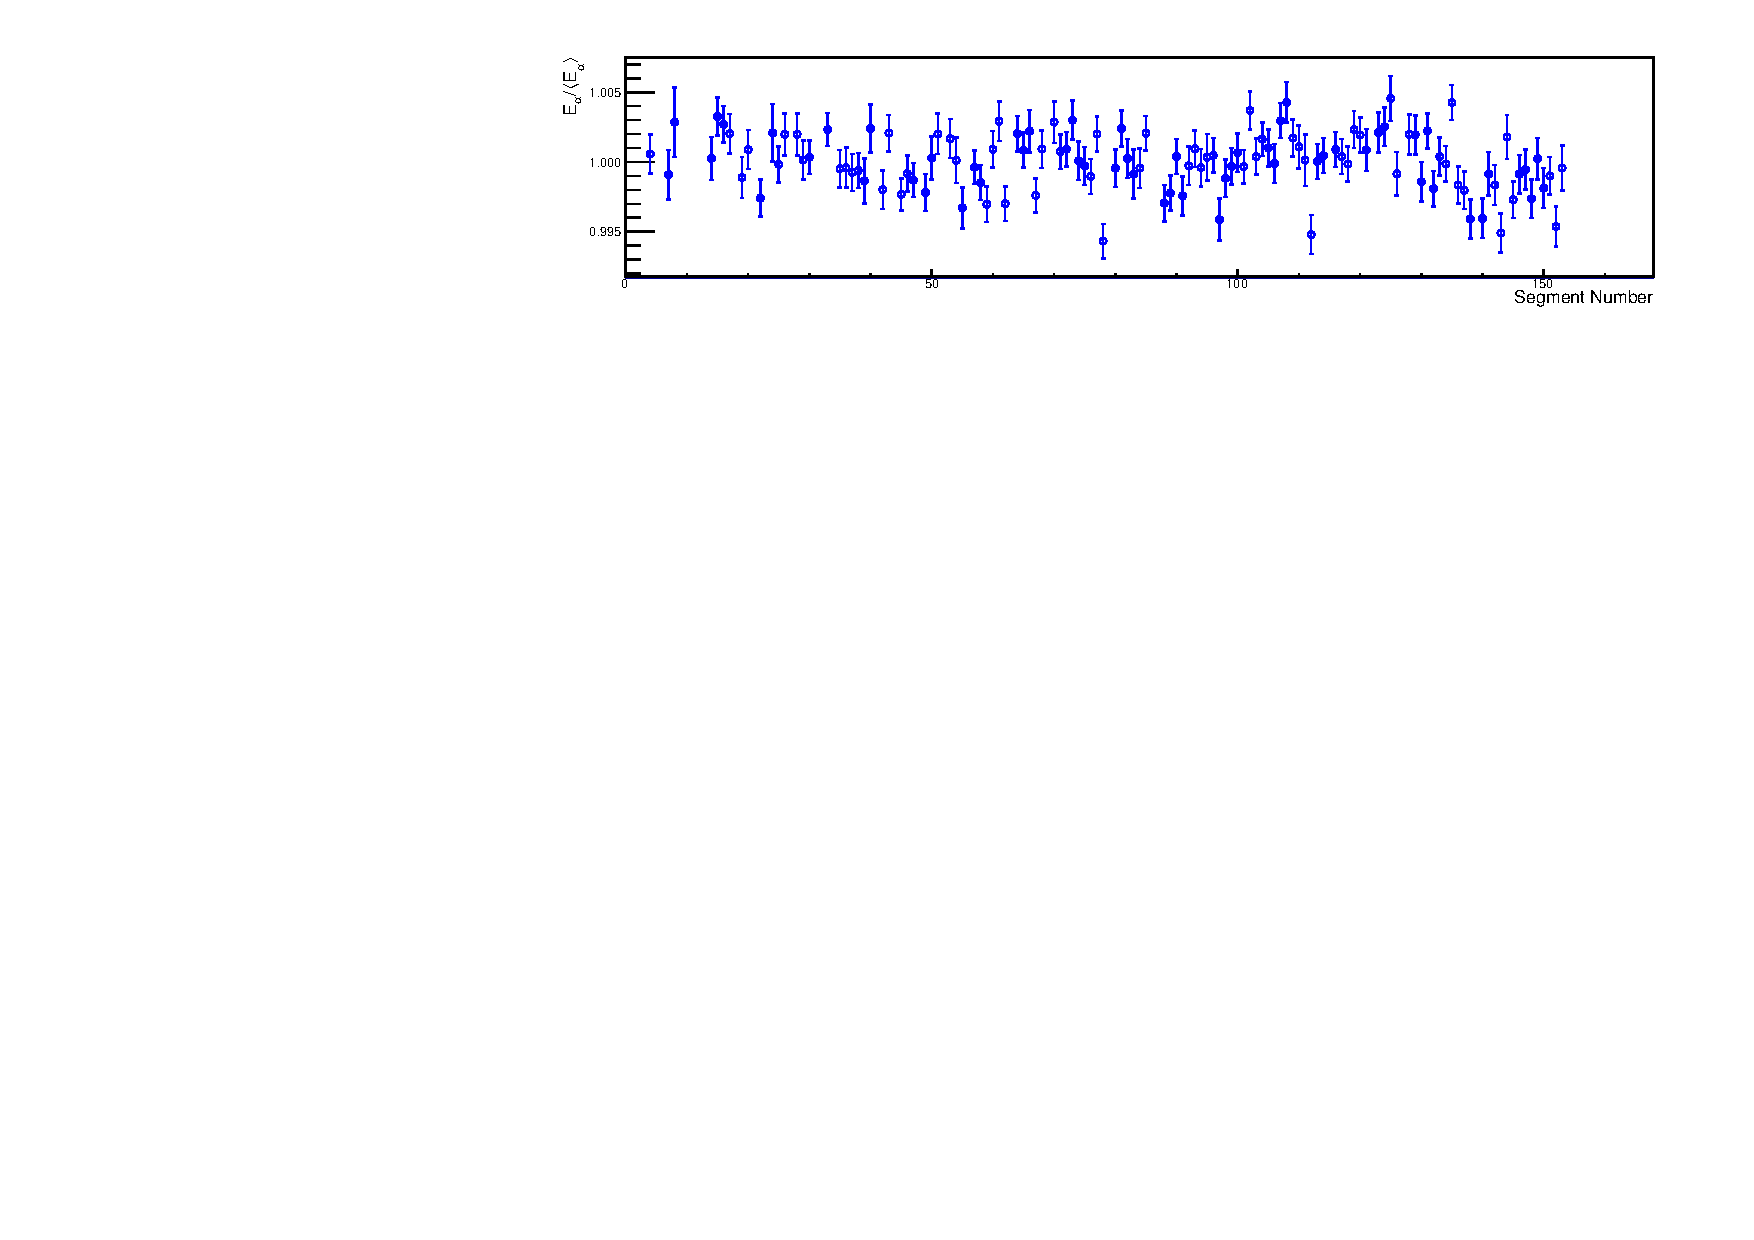
\includegraphics[width=1.05\textwidth]{figures/PubBiPo212EvsCell.pdf}
\caption{\label{fig:EvsCell212}Po-212 alpha energy versus segment number. The value is the mean of a Gaussian fit to the alpha energy peak and the error bar is the 1$\sigma$ width. Energy is normalized to the segment error-weighted average to highlight variations. Un-normalized weighted average energy is 1.0873$\pm$0.0001~MeV and $\chi^2$/NDF=296/122.}
\end{figure}
\begin{figure}[!h]
\centering
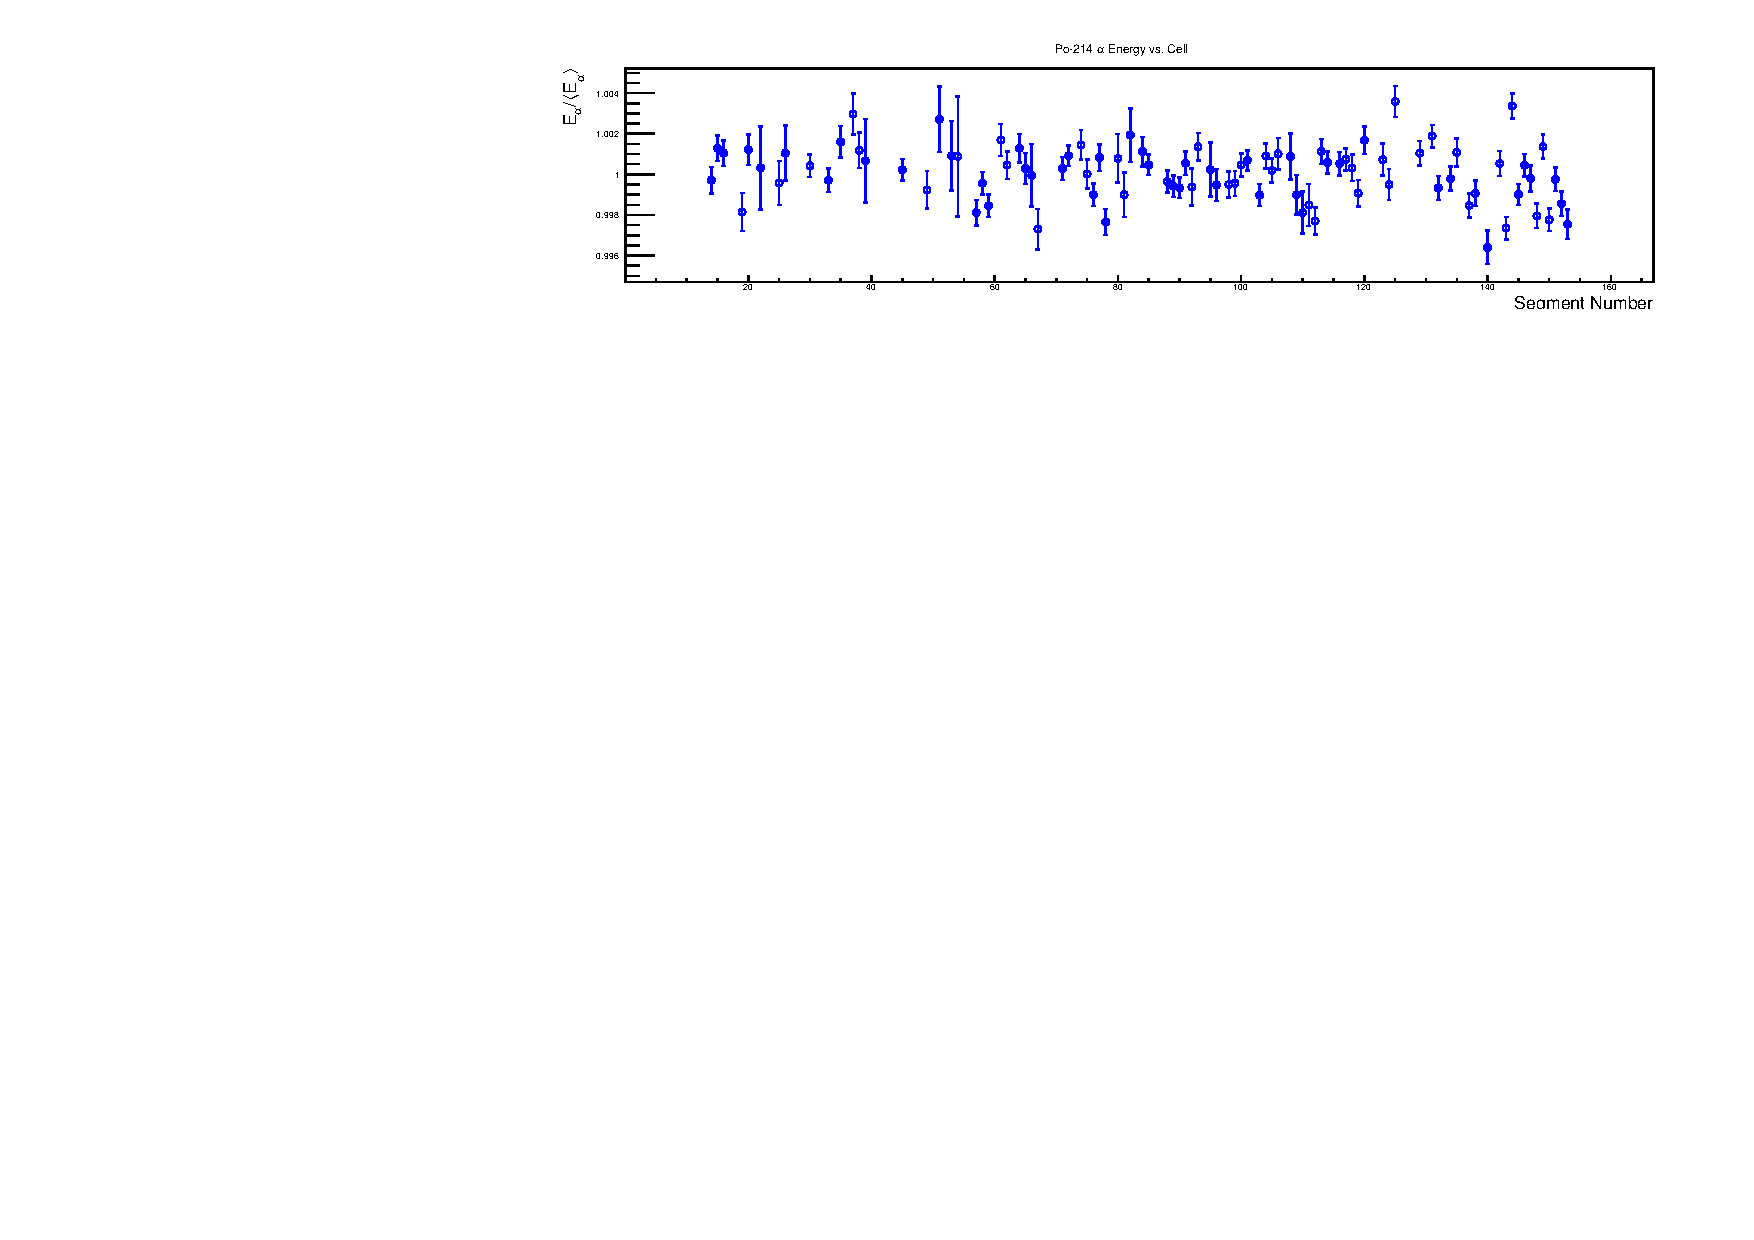
\includegraphics[width=1.05\textwidth]{figures/PubBiPo214EvsCell.pdf}
\caption{\label{fig:EvsCell214}Po-214 alpha energy versus segment number. The value is the mean of a Gaussian fit to the alpha energy peak and the error bar is the 1$\sigma$ width. Energy is normalized to the segment error-weighted average to highlight variations. Un-normalized weighted average energy is 0.8620$\pm$0.0001~MeV and $\chi^2$/NDF=169/122.} 
\end{figure}
\newpage
%------------------------------
\subsection{Energy resolution versus segment plots}
\begin{figure}[!h]
\centering
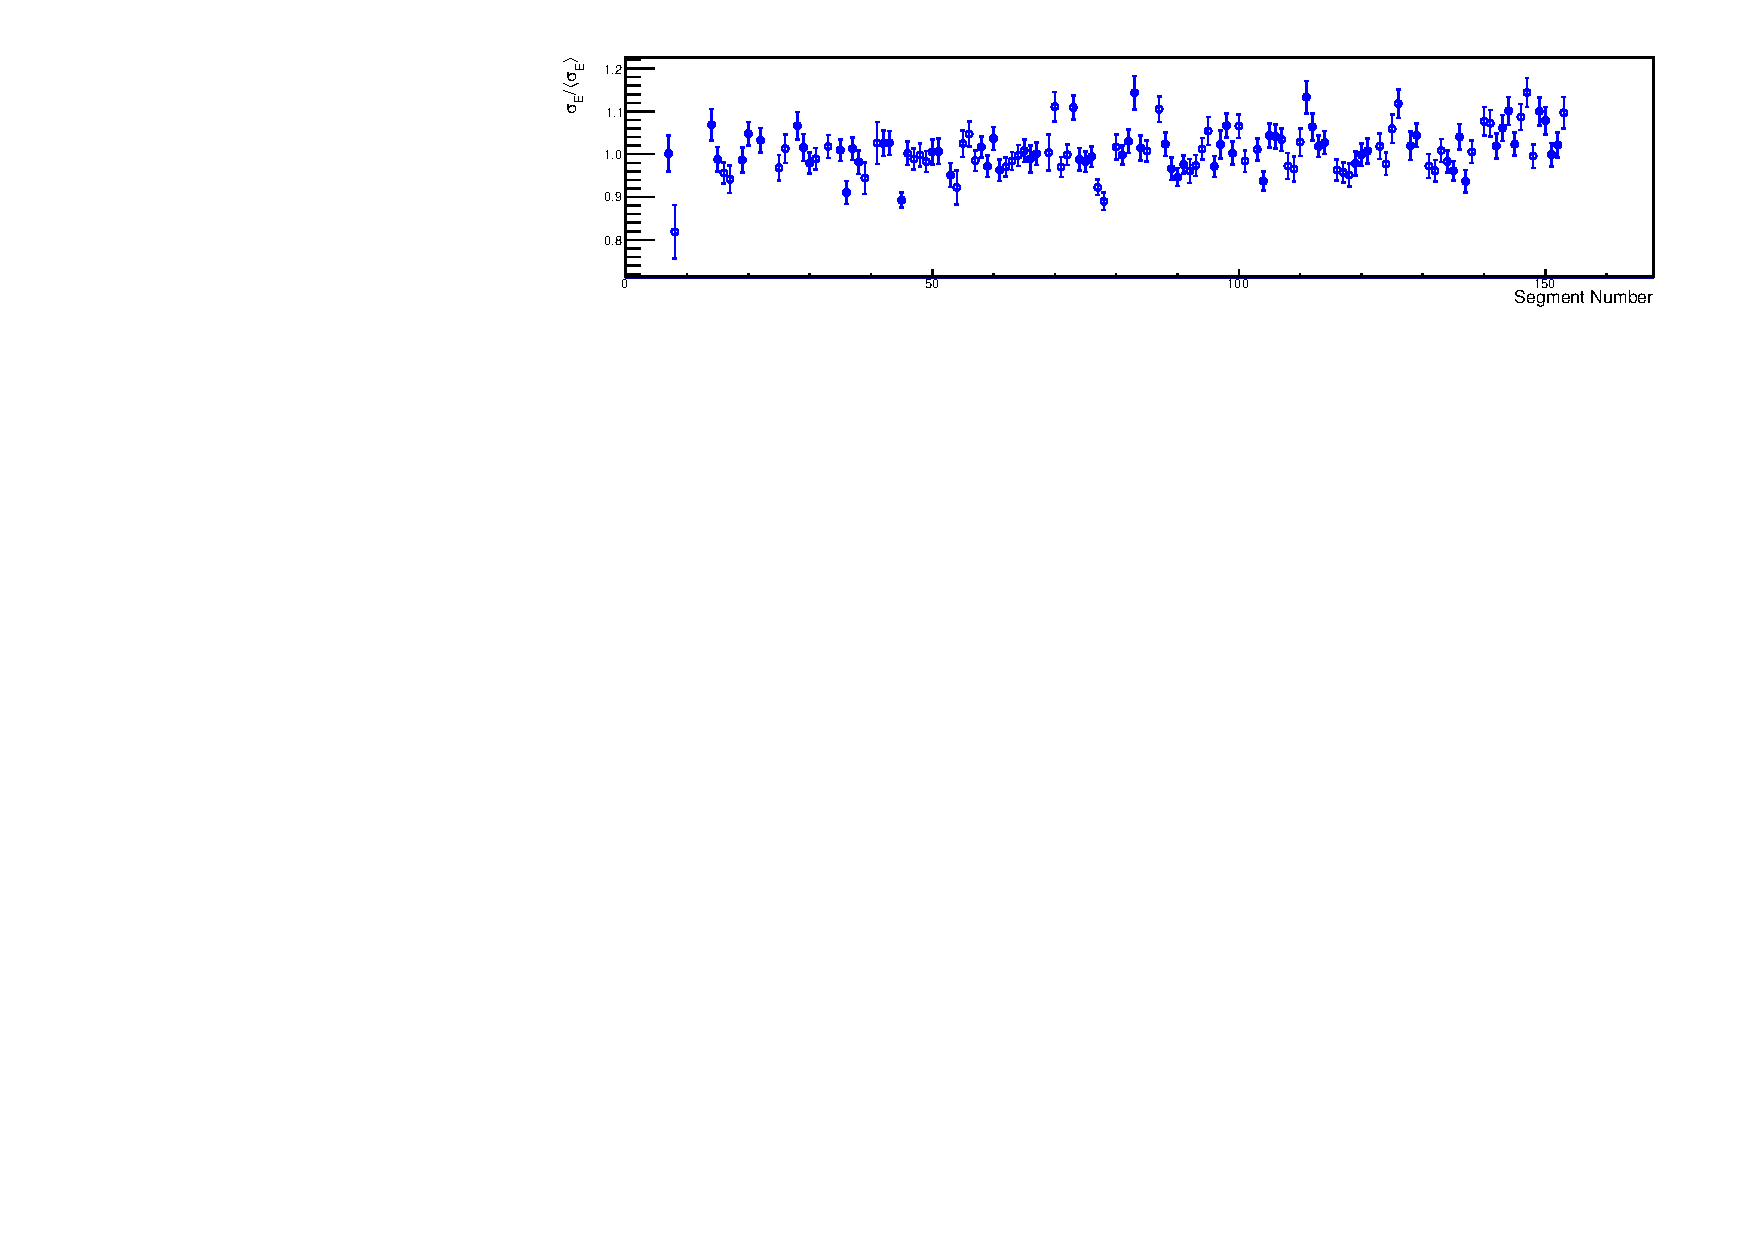
\includegraphics[width=1.05\textwidth]{figures/PubBiPo212EresvsCell.pdf}
\caption{\label{fig:EresvsCell212}Energy resolution versus segment using the alpha from Po-212 decay. The values are the 1$\sigma$ widths of a Gaussian fits to the alpha energy peaks and the error bars are the error on these values from the fit. Values are normalized to the segment error-weighted average to highlight variations. Un-normalized weighted average energy width is 0.0488$\pm$0.0001~MeV and $\chi^2$/NDF=391/122. Segment 8 has been seen to be problematic. In general, the higher width segments are those outfitted with ET tubes.}
\end{figure}
\begin{figure}[!h]
\centering
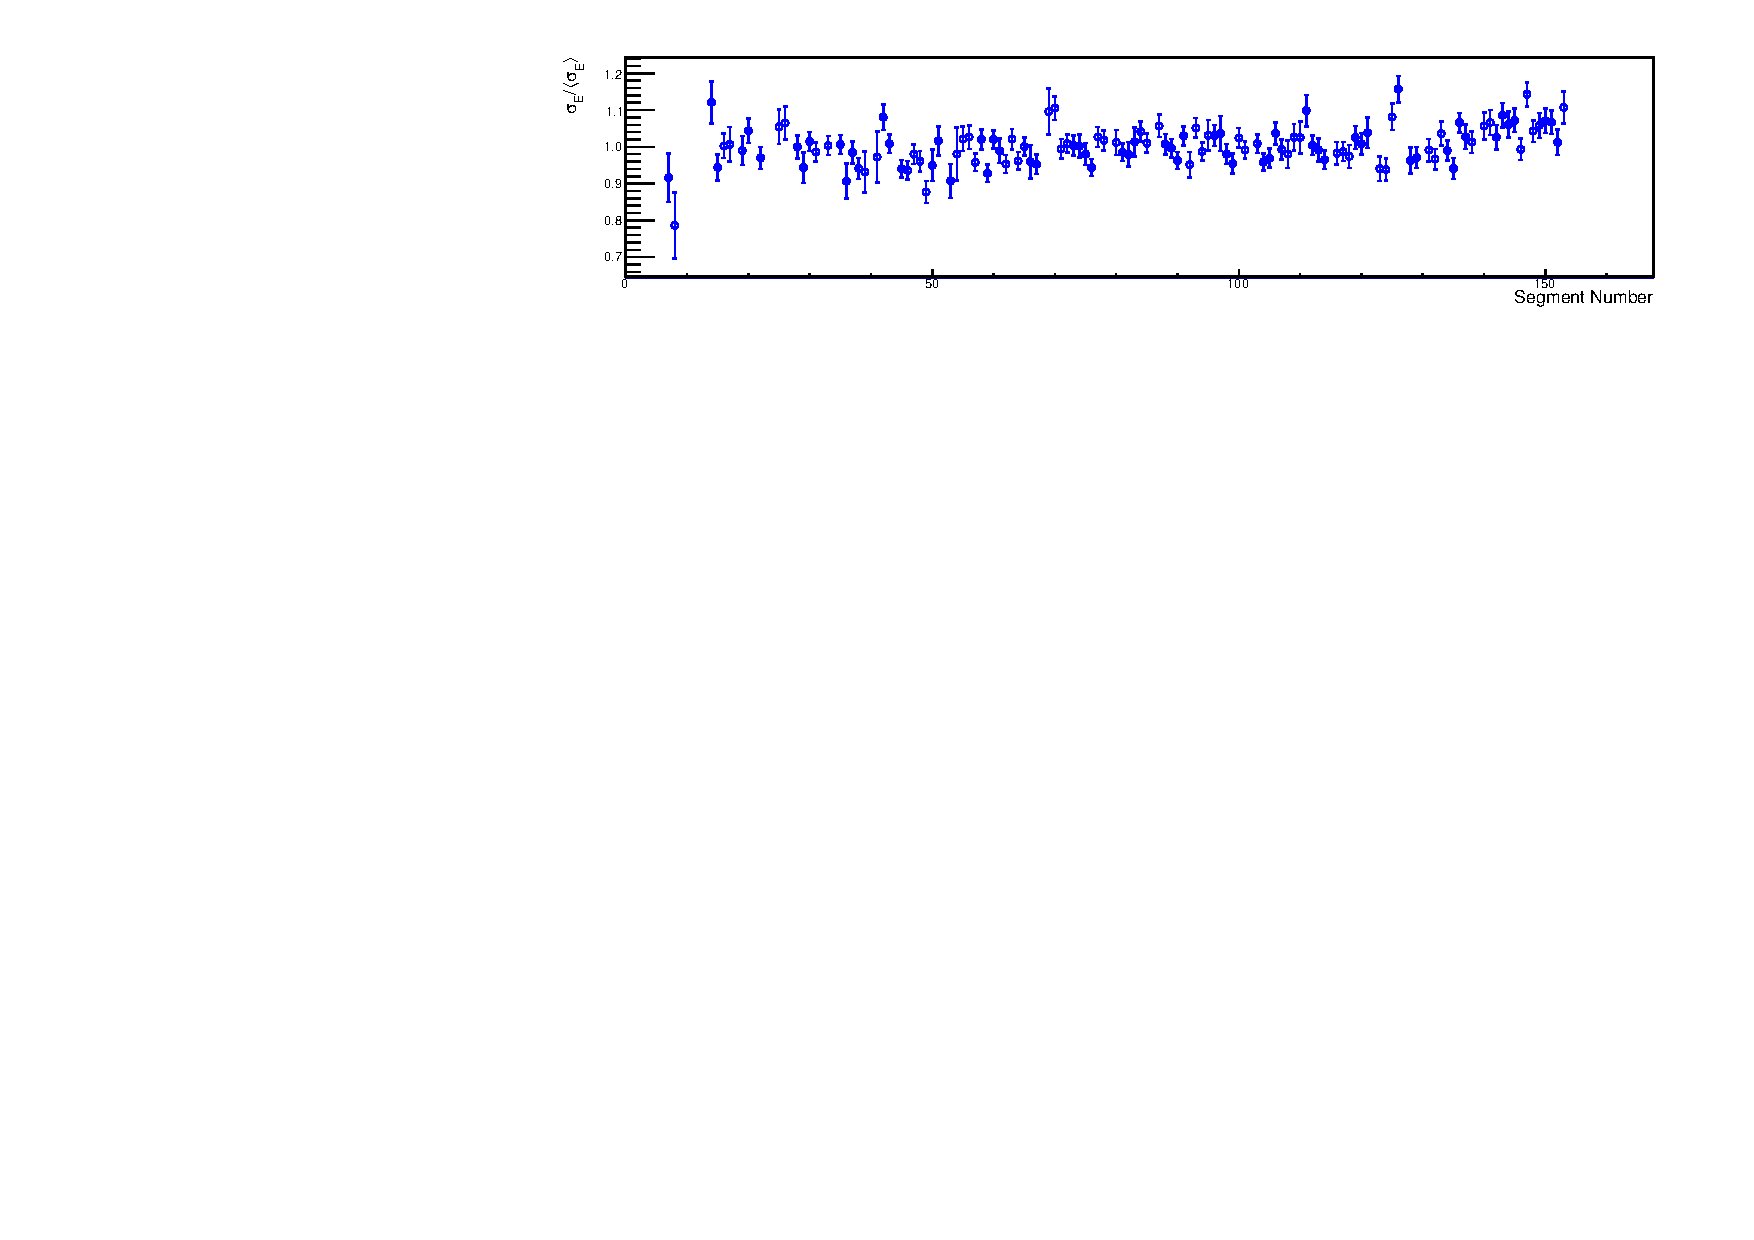
\includegraphics[width=1.05\textwidth]{figures/PubBiPo214EresvsCell.pdf}
\caption{\label{fig:EresvsCell214}Energy resolution versus segment using the alpha from Po-214 decay. The values are the 1$\sigma$ widths of a Gaussian fits to the alpha energy peaks and the error bars are the error on these values from the fit. Values are normalized to the segment error-weighted average to highlight variations. Un-normalized weighted average energy width is 0.0427$\pm$0.0001~MeV and $\chi^2$/NDF=272/122. Segment 8 has been seen to be problematic. In general, the higher width segments are those outfitted with ET tubes.}
\end{figure}
\newpage
%------------------------------
\subsection{Z-position resolution versus segment plots}
\begin{figure}[!h]
\centering
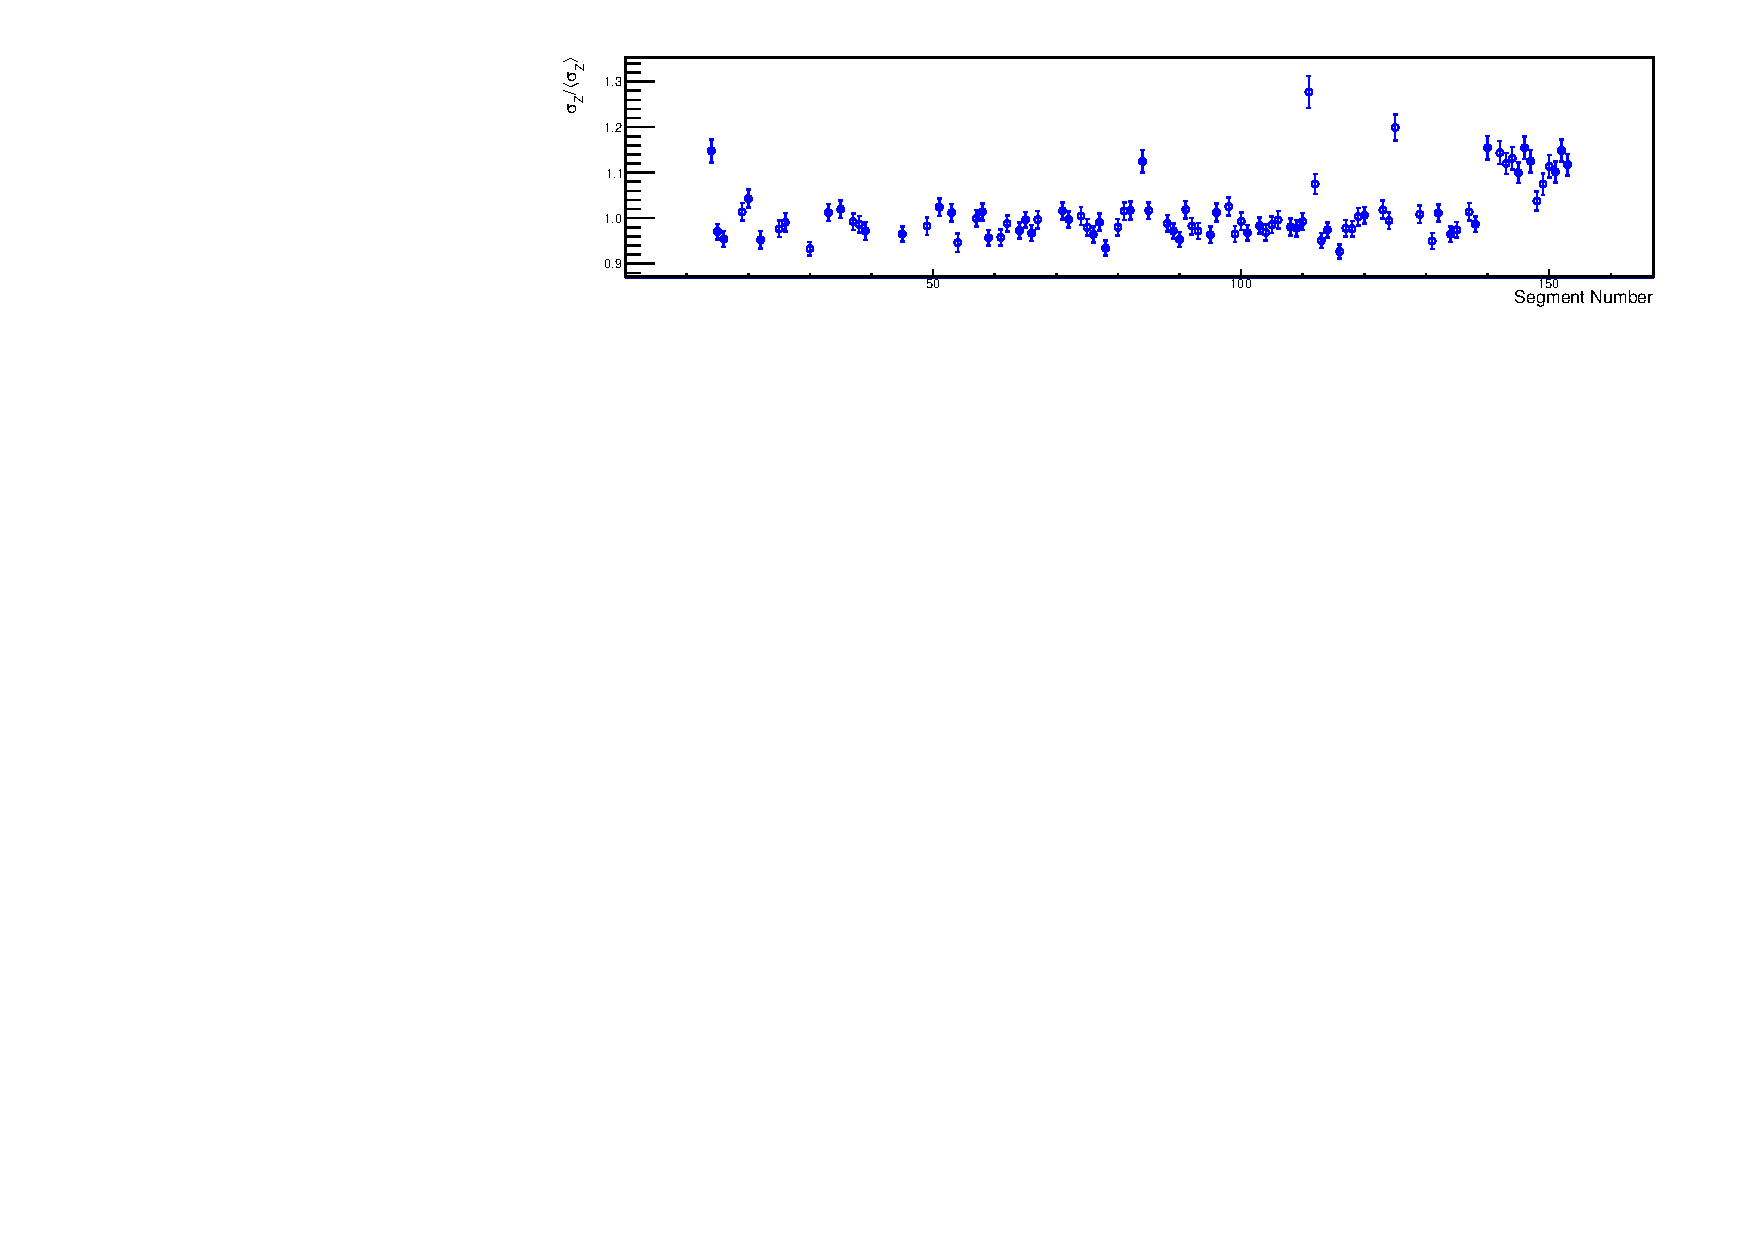
\includegraphics[width=1.05\textwidth]{figures/PubBiPo212dZWidthvsCell.pdf}
\caption{\label{fig:ZresvsCell212}Z-position resolution versus segment using the beta, alpha from Bi-212, Po-212. The values are the 1$\sigma$ widths of a Gaussian fits to the alpha minus beta Z-distance distributions and the error bars are the error on these values from the fit. Values are normalized to the segment error-weighted average to highlight variations. Un-normalized weighted average $\Delta$Z width is 45.18$\pm$0.13~mm and $\chi^2$/NDF=429/122.}
\end{figure}
\begin{figure}[!h]
\centering
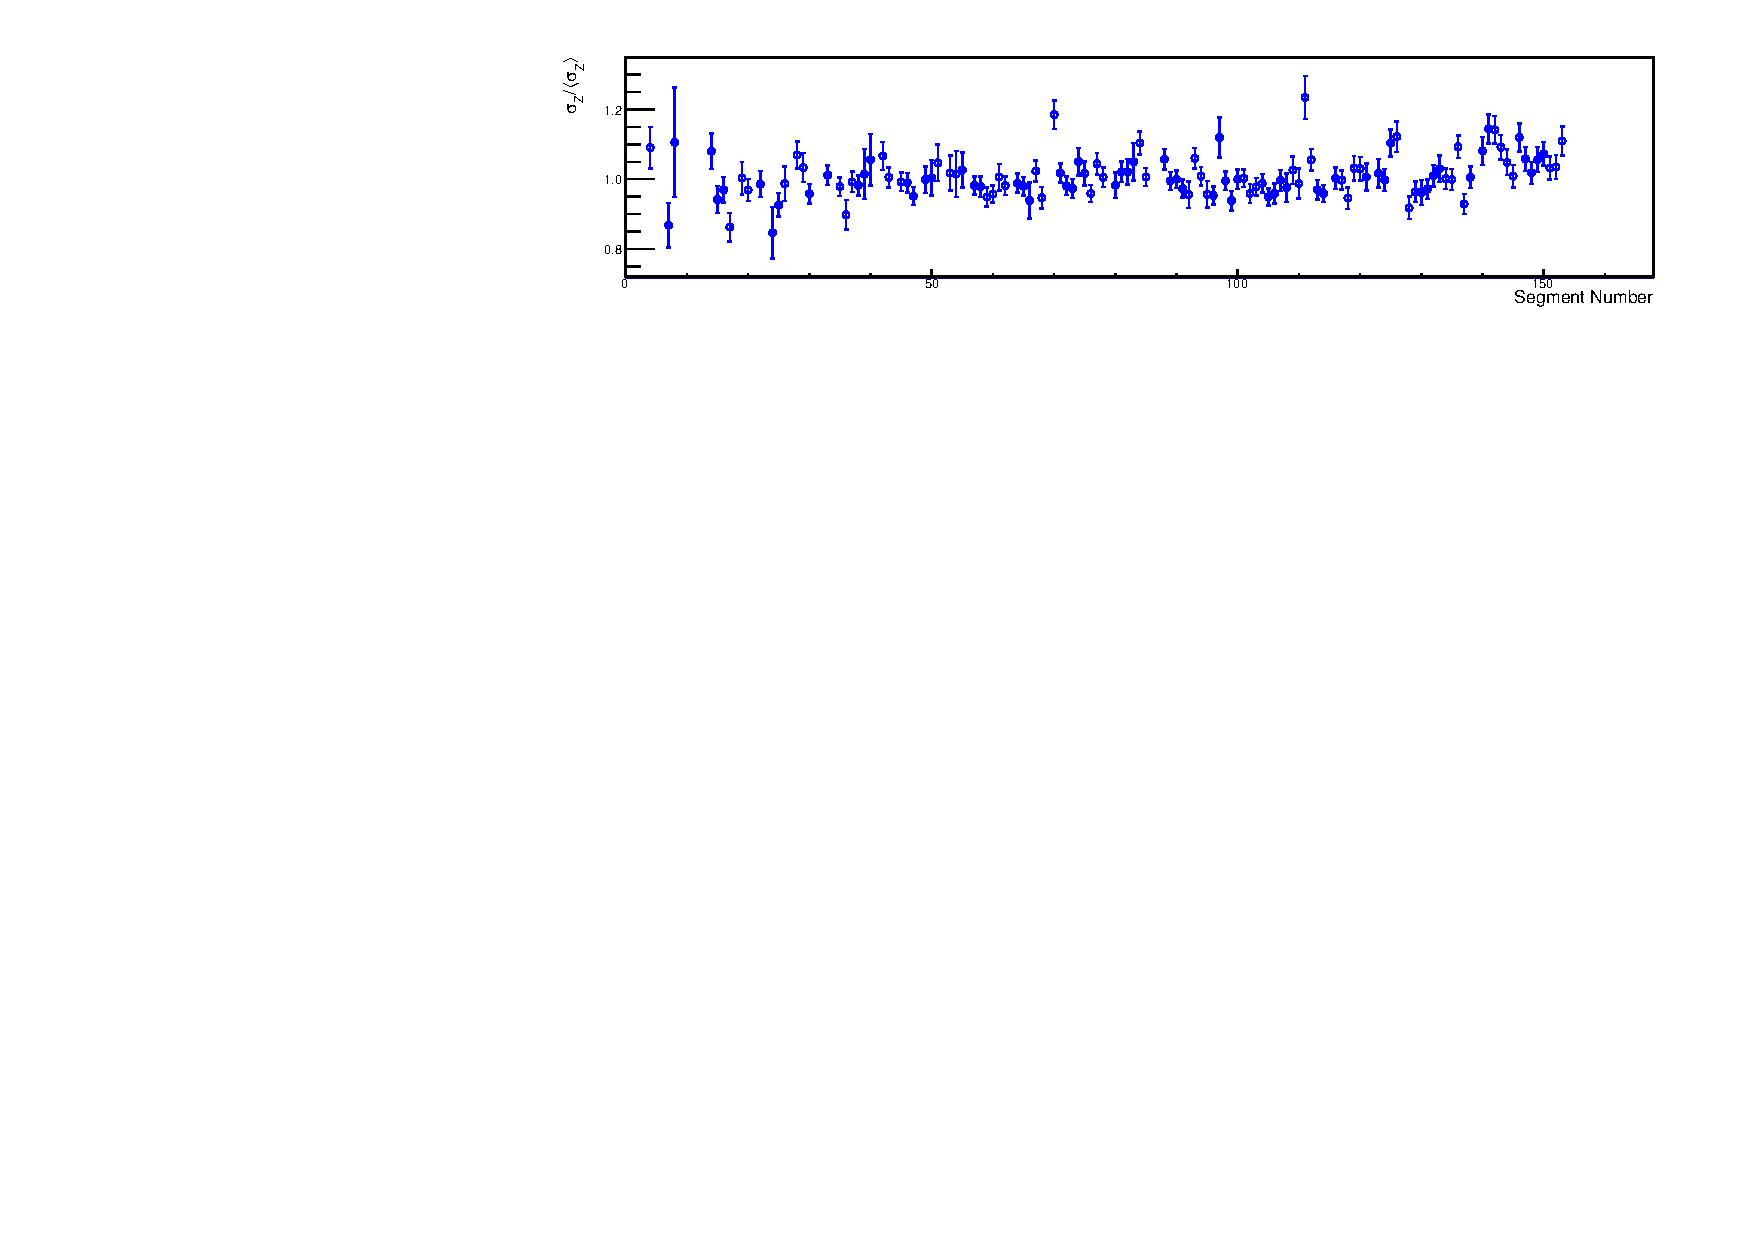
\includegraphics[width=1.05\textwidth]{figures/PubBiPo214dZWidthvsCell.pdf}
\caption{\label{fig:ZresvsCell214}Z-position resolution versus segment using the beta, alpha from Bi-214, Po-214. The values are the 1$\sigma$ widths of a Gaussian fits to the alpha minus beta Z-distance distributions and the error bars are the error on these values from the fit. Values are normalized to the segment error-weighted average to highlight variations. Un-normalized weighted average $\Delta$Z width is 52.71$\pm$0.17~mm and $\chi^2$/NDF=230/122. In general, the higher width segments are those outfitted with ET tubes.}
\end{figure}
\newpage
%------------------------------
\subsection{Z-distribution RMS width versus segment plots}
\begin{figure}[!h]
\centering
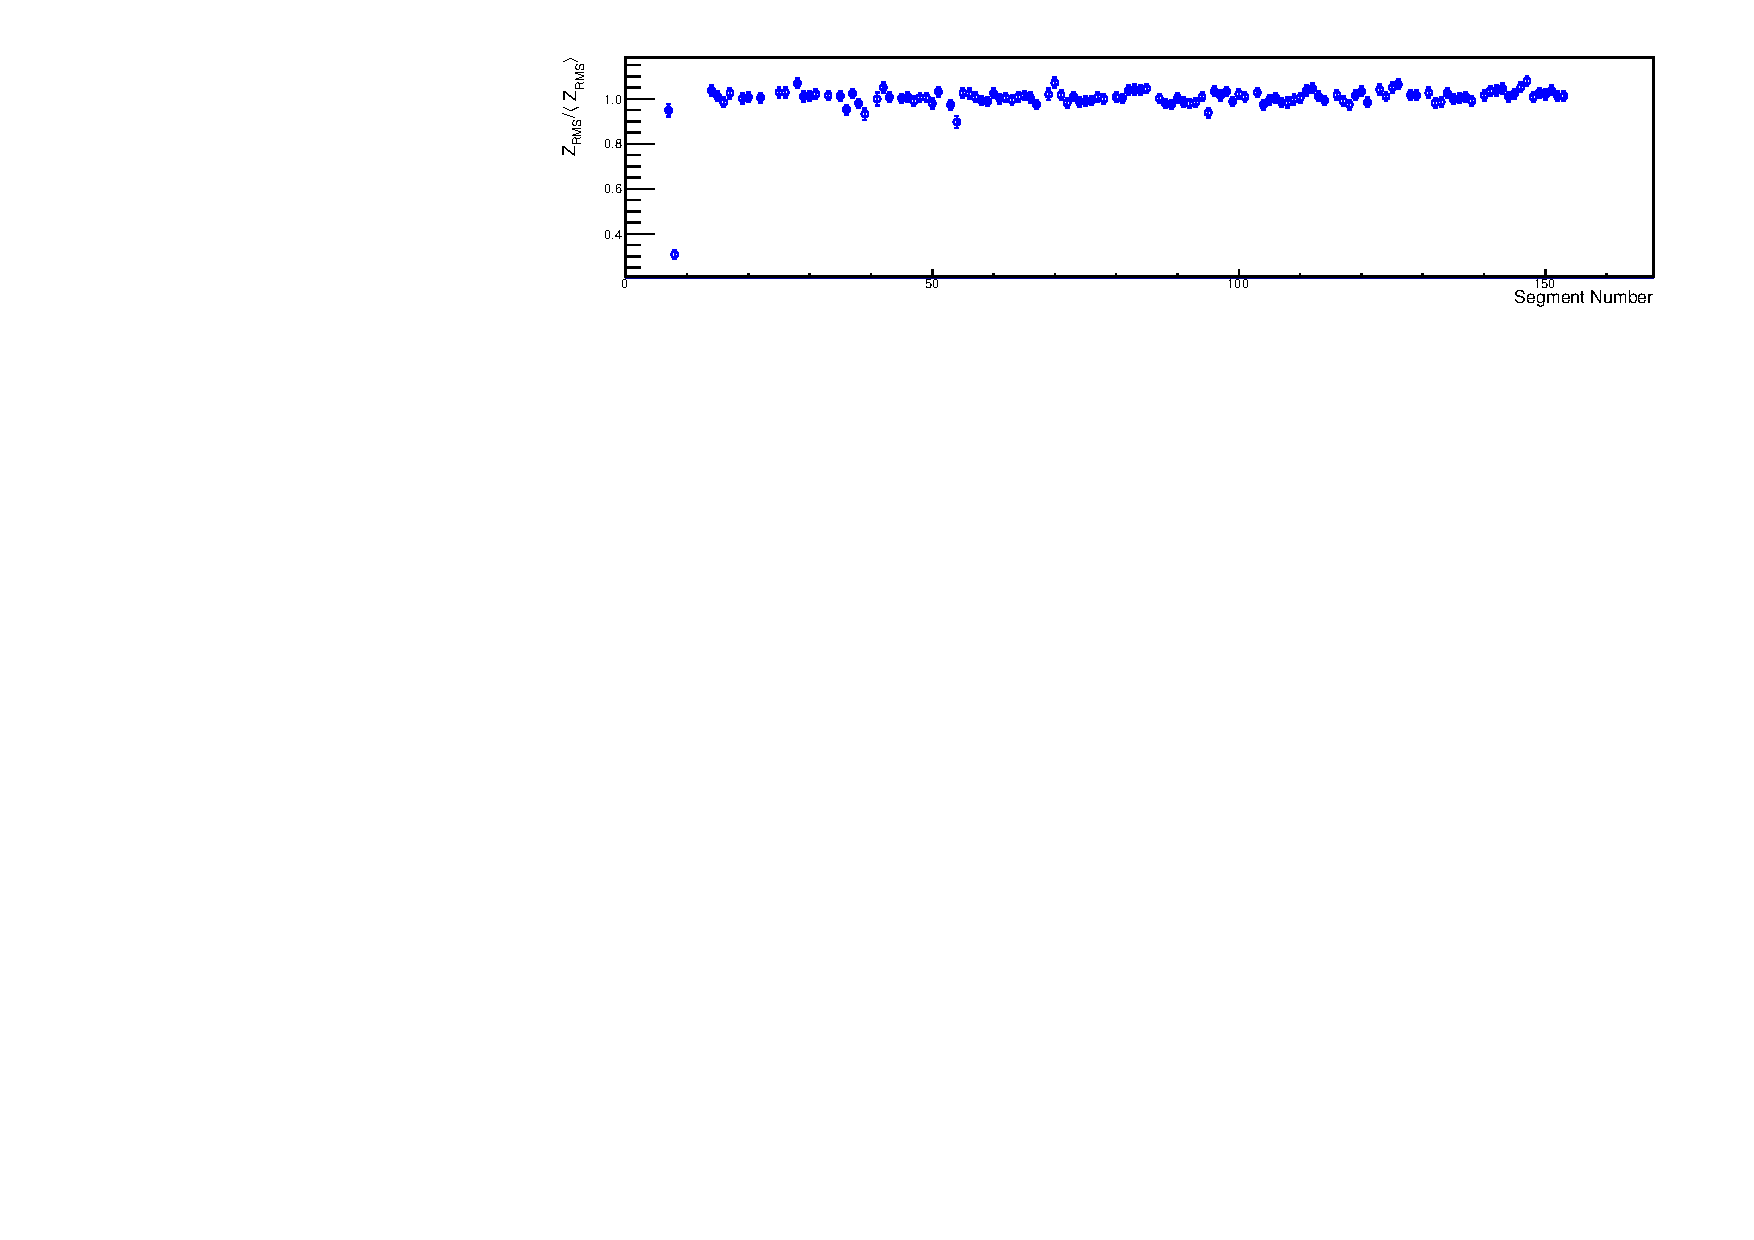
\includegraphics[width=1.05\textwidth]{figures/PubBiPo212ZRMSvsCell.pdf}
\caption{\label{fig:ZRMSvsCell212}RMS width of Z-distribution of Po-212 alphas versus segment. The error bars are the errors assigned by ROOT to the RMS values of the histograms. Values are normalized to the segment error-weighted average to highlight variations. Un-normalized weighted average Z$_{RMS}$ width is 345.5$\pm$0.7~mm and $\chi^2$/NDF=1730/122. Segment 8 has been seen to be problematic.}
\end{figure}
\begin{figure}[!h]
\centering
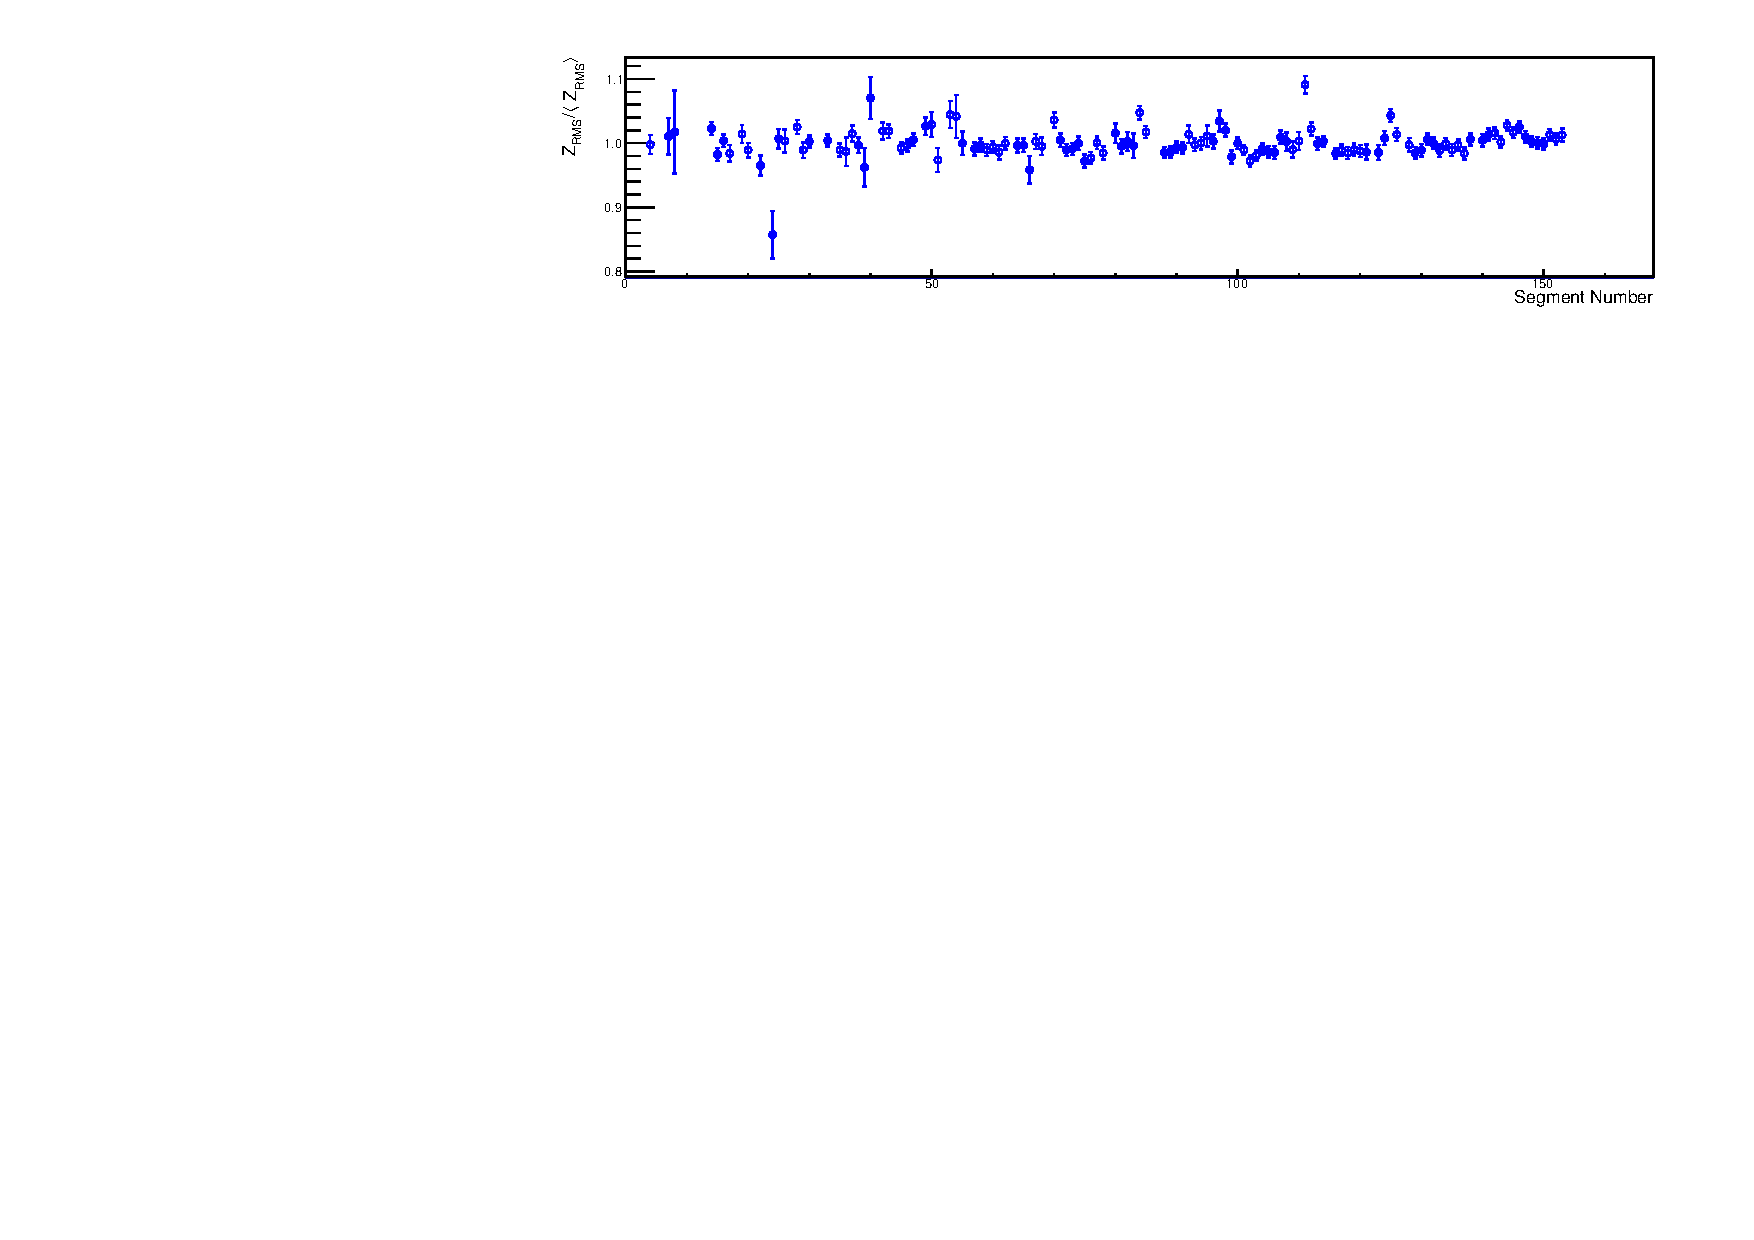
\includegraphics[width=1.05\textwidth]{figures/PubBiPo214ZRMSvsCell.pdf}
\caption{\label{fig:ZRMSvsCell214}RMS width of Z-distribution of Po-214 alphas versus segment. The error bars are the errors assigned by ROOT to the RMS values of the histograms. Values are normalized to the segment error-weighted average to highlight variations. Un-normalized weighted average Z$_{RMS}$ width is 349.1$\pm$0.6~mm and $\chi^2$/NDF=153/122.}
\end{figure}
\newpage
%------------------------------
\subsection{Energy versus time plots}
\begin{figure}[!h]
\centering
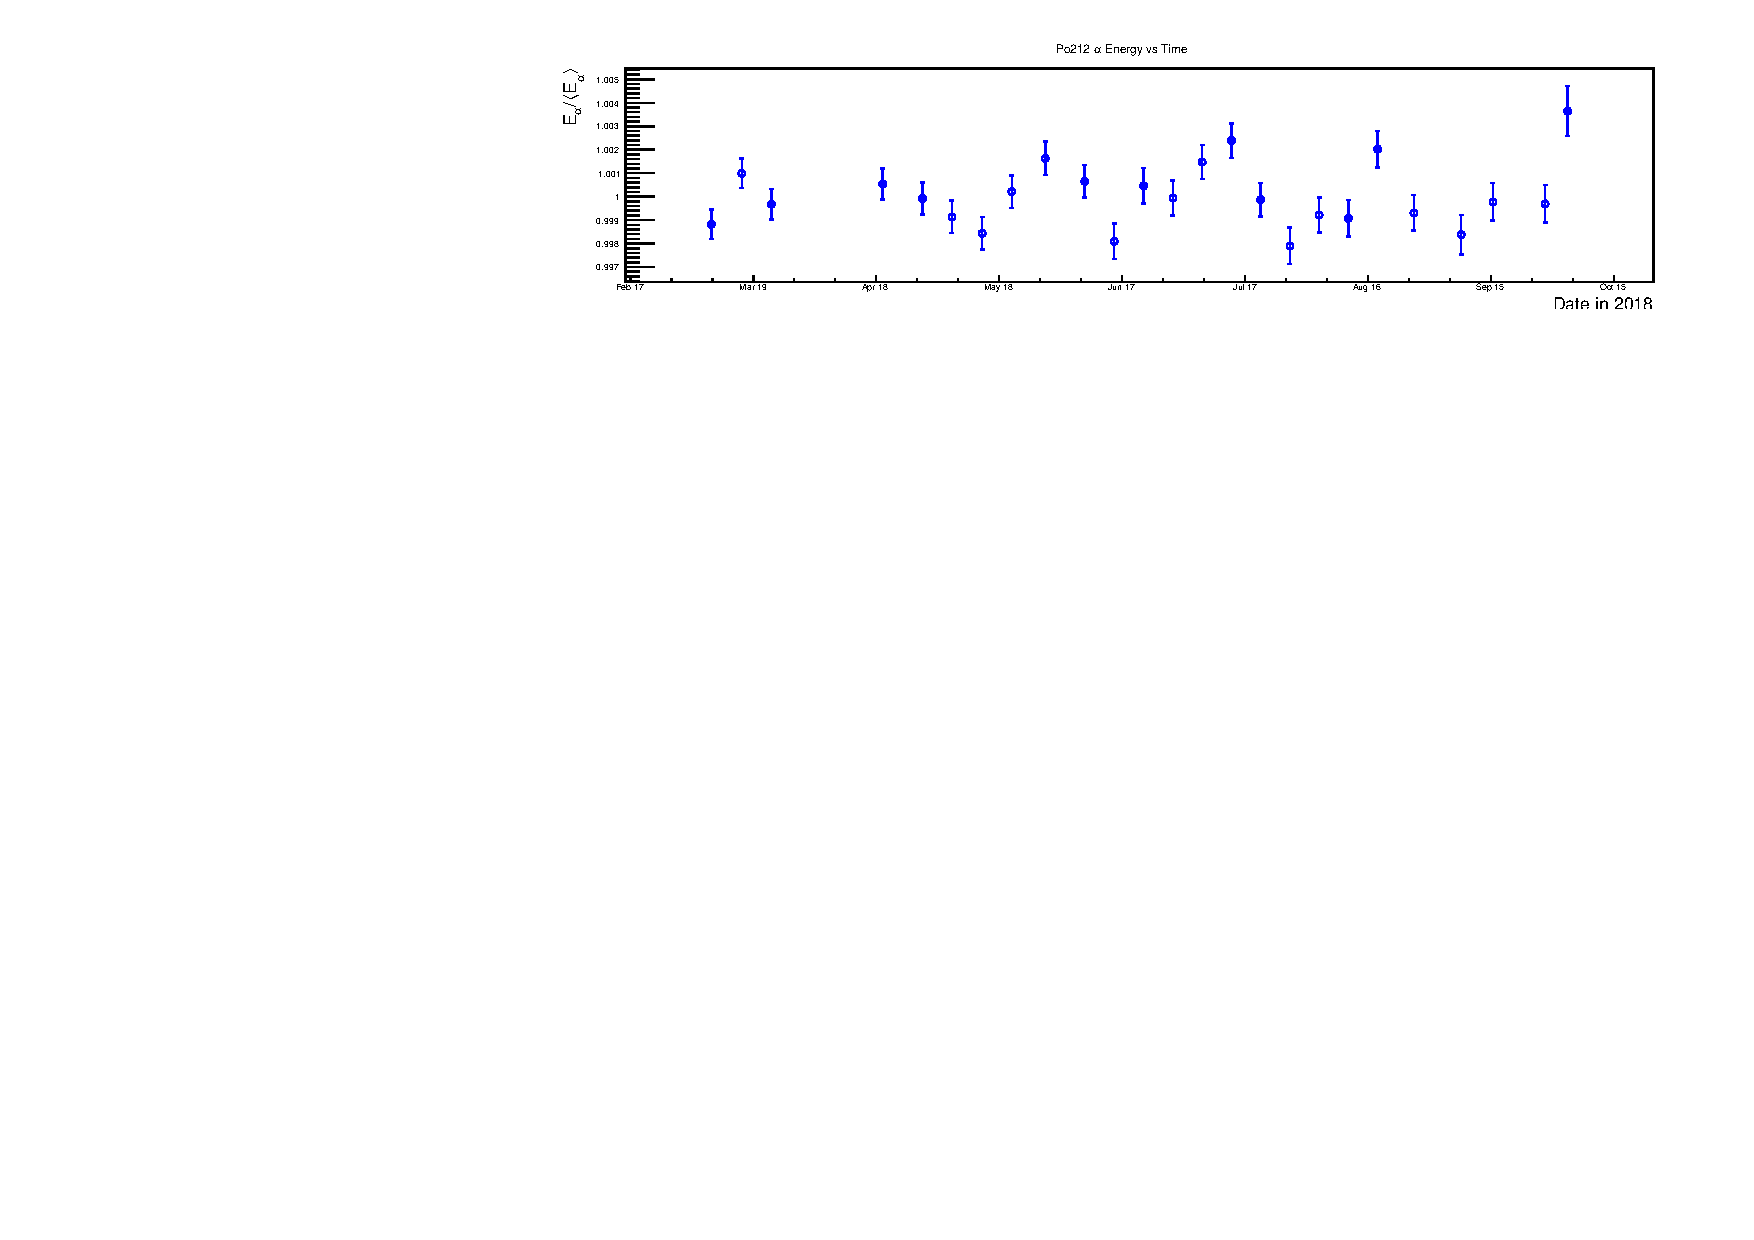
\includegraphics[width=1.05\textwidth]{figures/PubBiPo212EvsT.pdf}
\caption{\label{fig:EvsT212}Po-212 detector averaged alpha energy versus time. The value is the mean of a Gaussian fit to the alpha energy peak and the error bar is the 1$\sigma$ width. Energy is normalized to the segment error-weighted average to highlight variations. Un-normalized weighted average energy is 1.08735$\pm$0.00015~MeV and $\chi^2$/NDF=68.5/60. }
\end{figure}
\begin{figure}[!h]
\centering
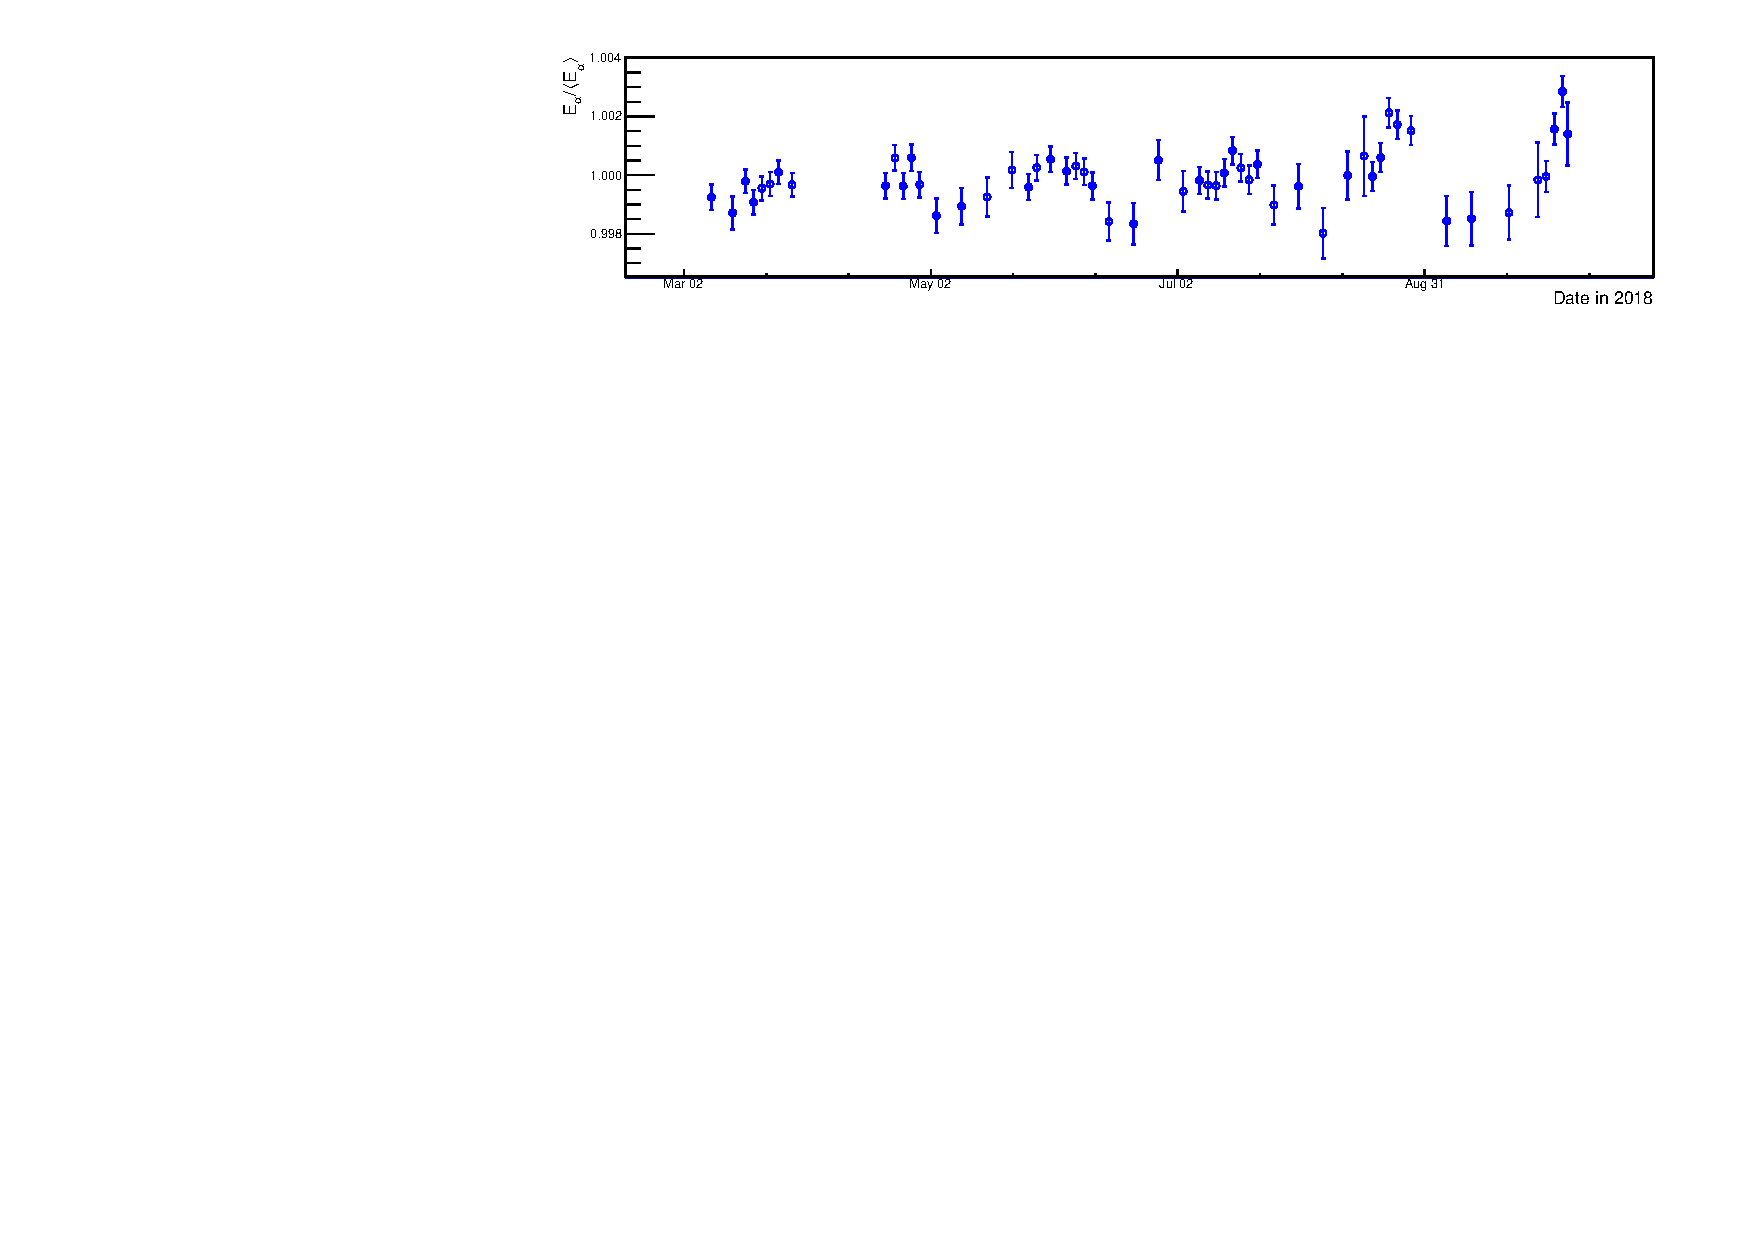
\includegraphics[width=1.05\textwidth]{figures/PubBiPo214EvsT.pdf}
\caption{\label{fig:EvsT214}Po-214 detector averaged alpha energy versus time. The value is the mean of a Gaussian fit to the alpha energy peak and the error bar is the 1$\sigma$ width. Energy is normalized to the segment error-weighted average to highlight variations. Un-normalized weighted average energy is 0.8619$\pm$0.0001~MeV and $\chi^2$/NDF=77.1/60. The periods of increased error bar occur during reactor on when accidental backgrounds for this BiPo-214 decay process are much larger. The BiPo-212 decay has almost no accidental backgrounds due to the relatively short lifetime of Po-212 (299~ns).}
\end{figure}
\newpage
%------------------------------
\subsection{Energy resolution versus time plots}
\begin{figure}[!h]
\centering
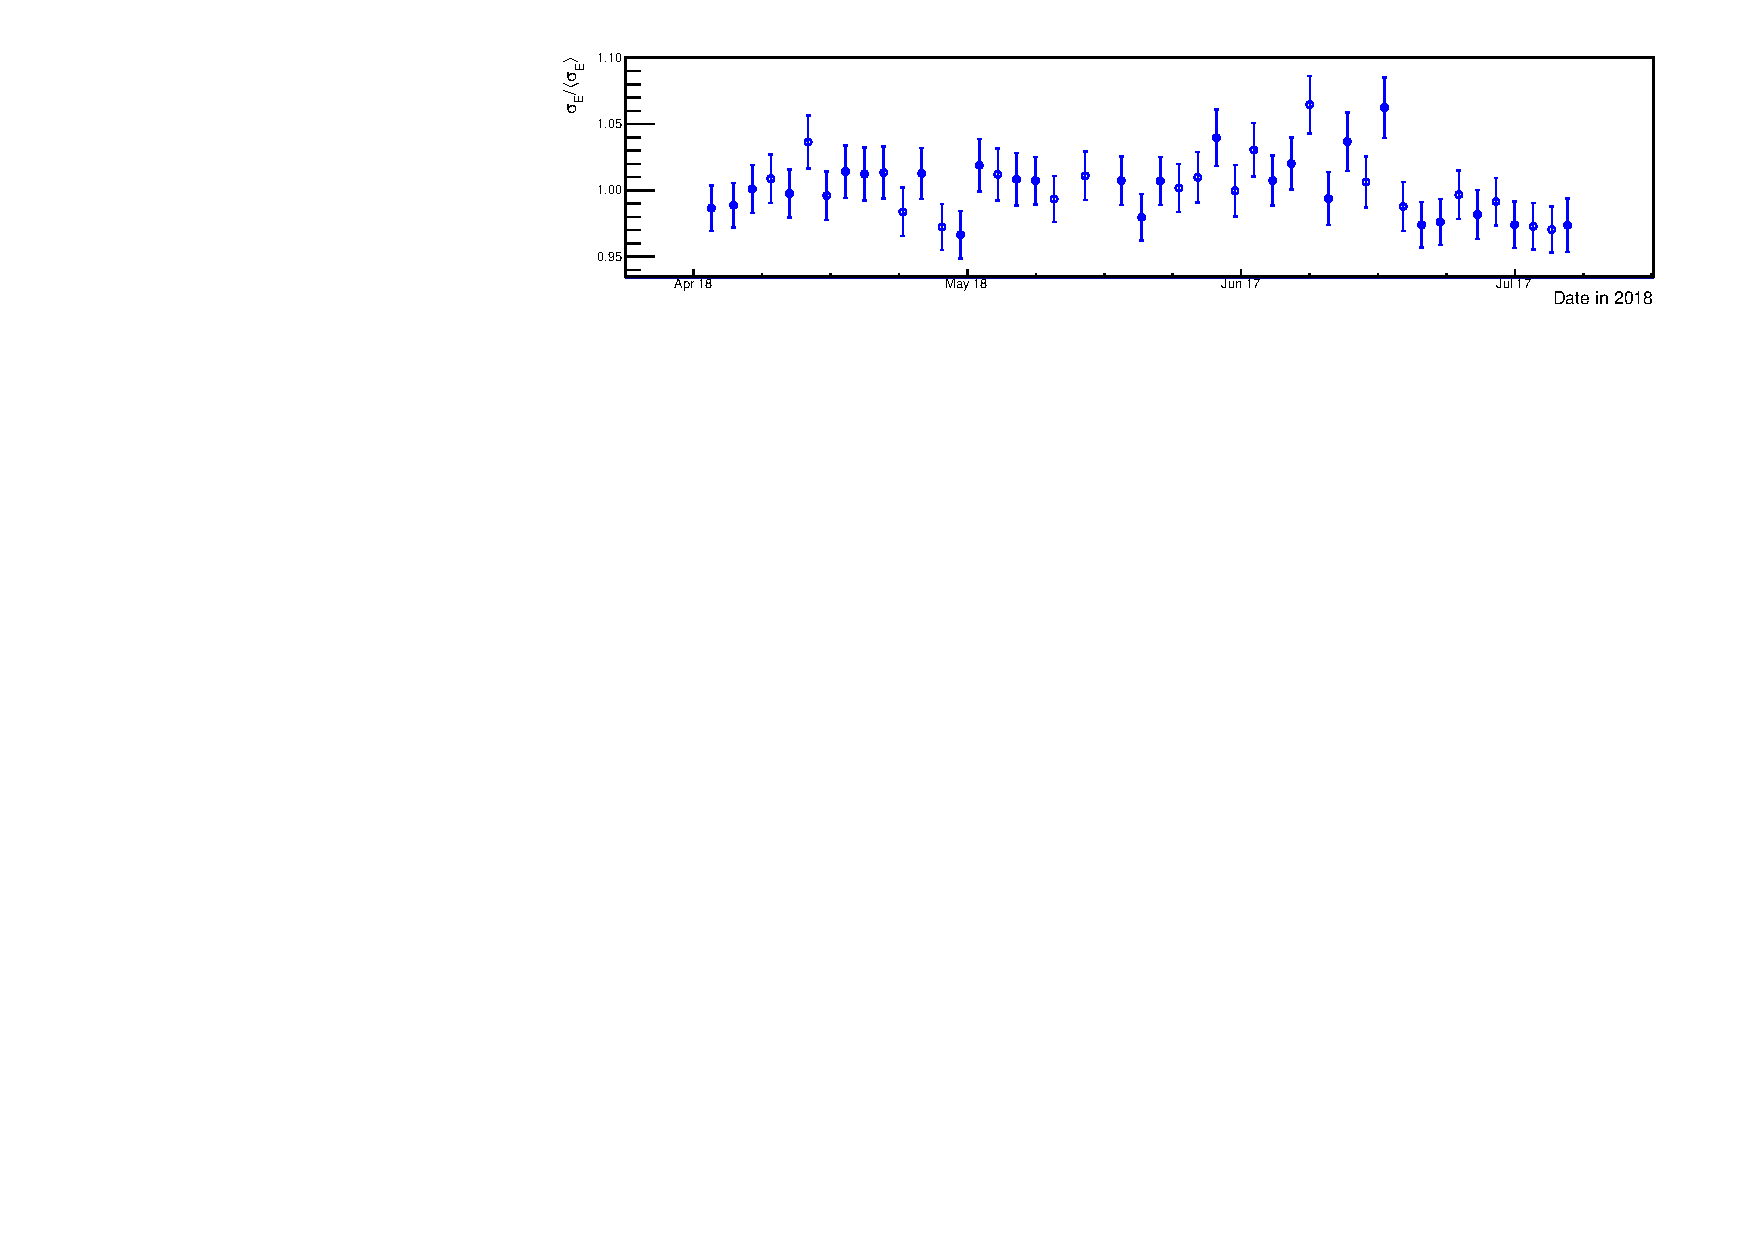
\includegraphics[width=1.05\textwidth]{figures/PubBiPo212EresvsT.pdf}
\caption{\label{fig:EresvsT212}Detector averaged energy resolution versus time using the alpha from Po-212 decay. The values are the 1$\sigma$ widths of a Gaussian fits to the alpha energy peaks and the error bars are the error on these values from the fit. Values are normalized to the segment error-weighted average to highlight variations. Un-normalized weighted average energy width is 0.0490$\pm$0.0001~MeV and $\chi^2$/NDF=152/60.}
\end{figure}
\begin{figure}[!h]
\centering
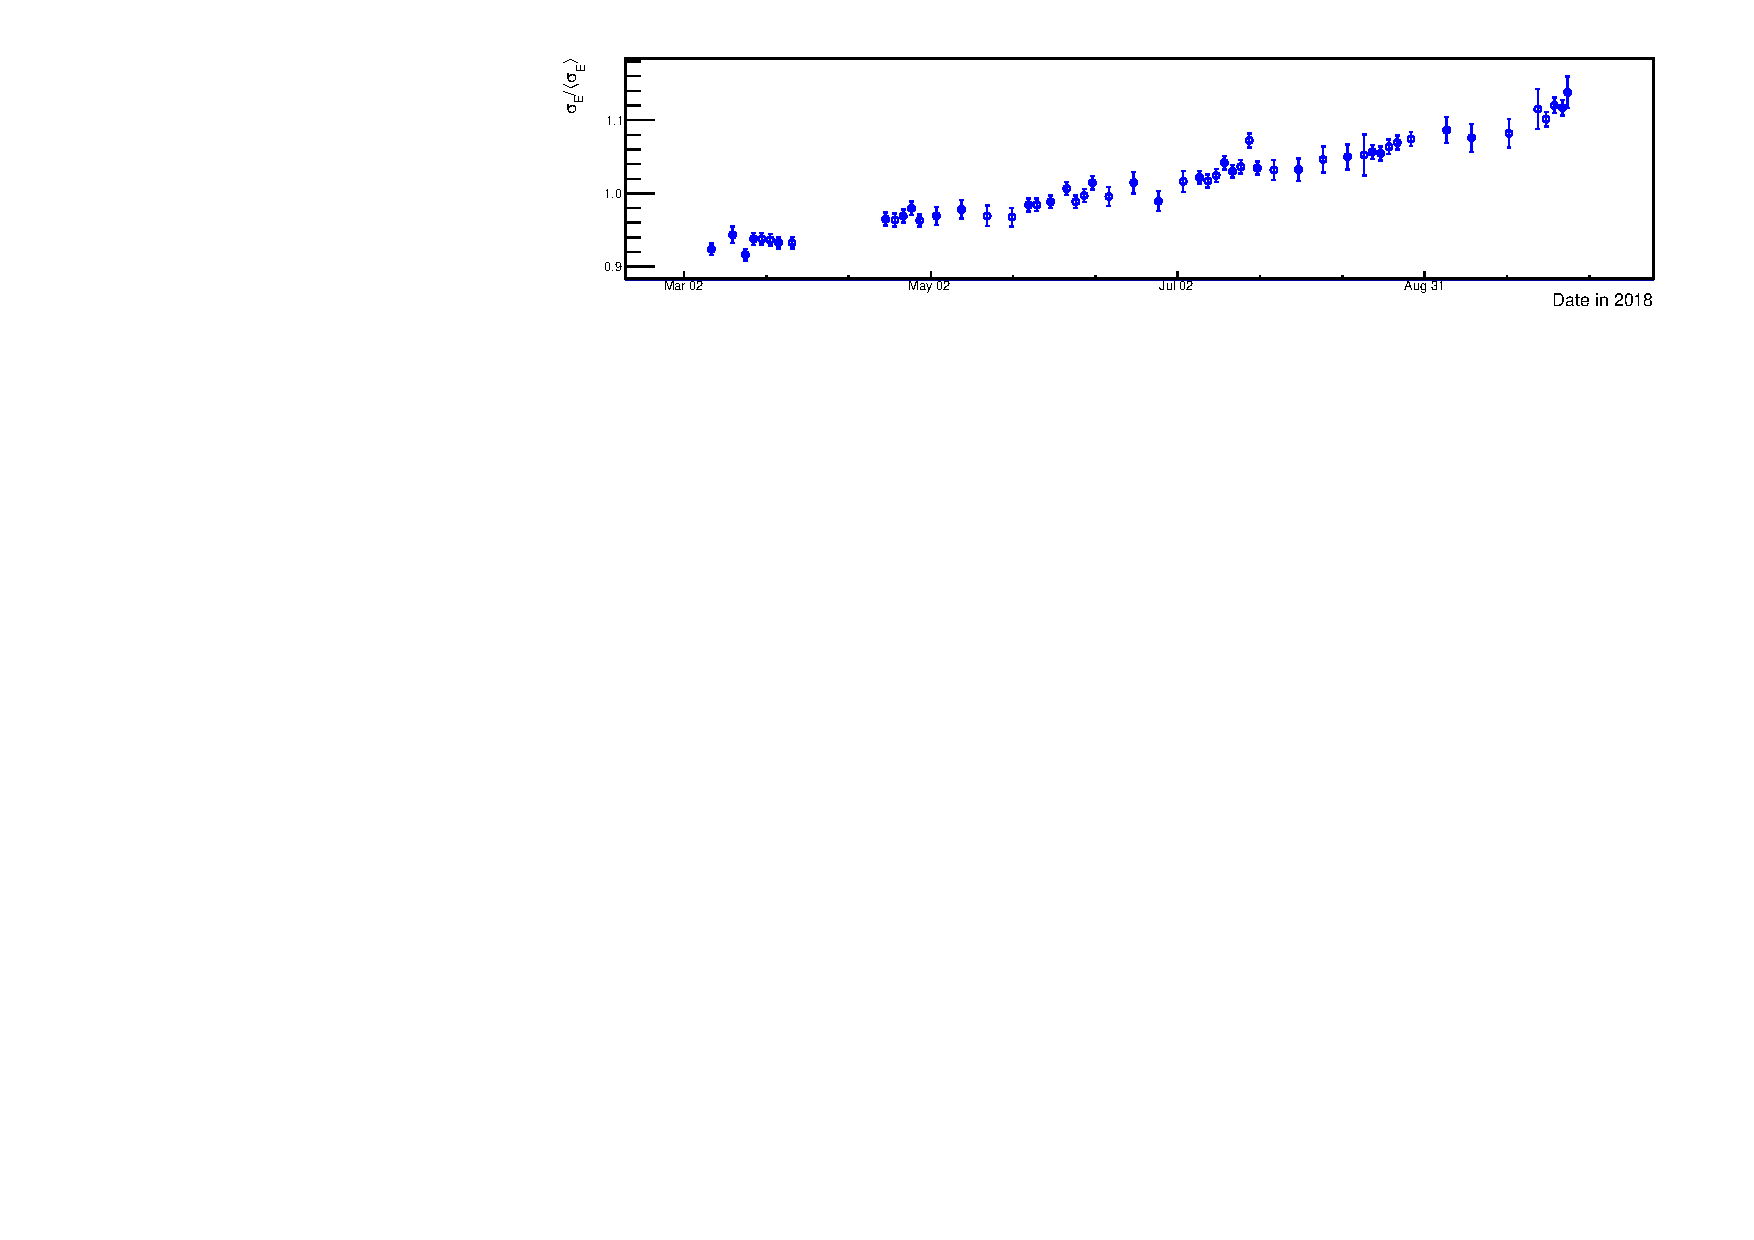
\includegraphics[width=1.05\textwidth]{figures/PubBiPo214EresvsT.pdf}
\caption{\label{fig:EresvsT214}Detector averaged energy resolution versus time using the alpha from Po-214 decay. The values are the 1$\sigma$ widths of a Gaussian fits to the alpha energy peaks and the error bars are the error on these values from the fit. Values are normalized to the segment error-weighted average to highlight variations. Un-normalized weighted average energy width is 0.0427$\pm$0.0001~MeV and $\chi^2$/NDF=165/60.}
\end{figure}
\newpage
%------------------------------
\subsection{Z-distribution RMS width versus time plots}
\begin{figure}[!h]
\centering
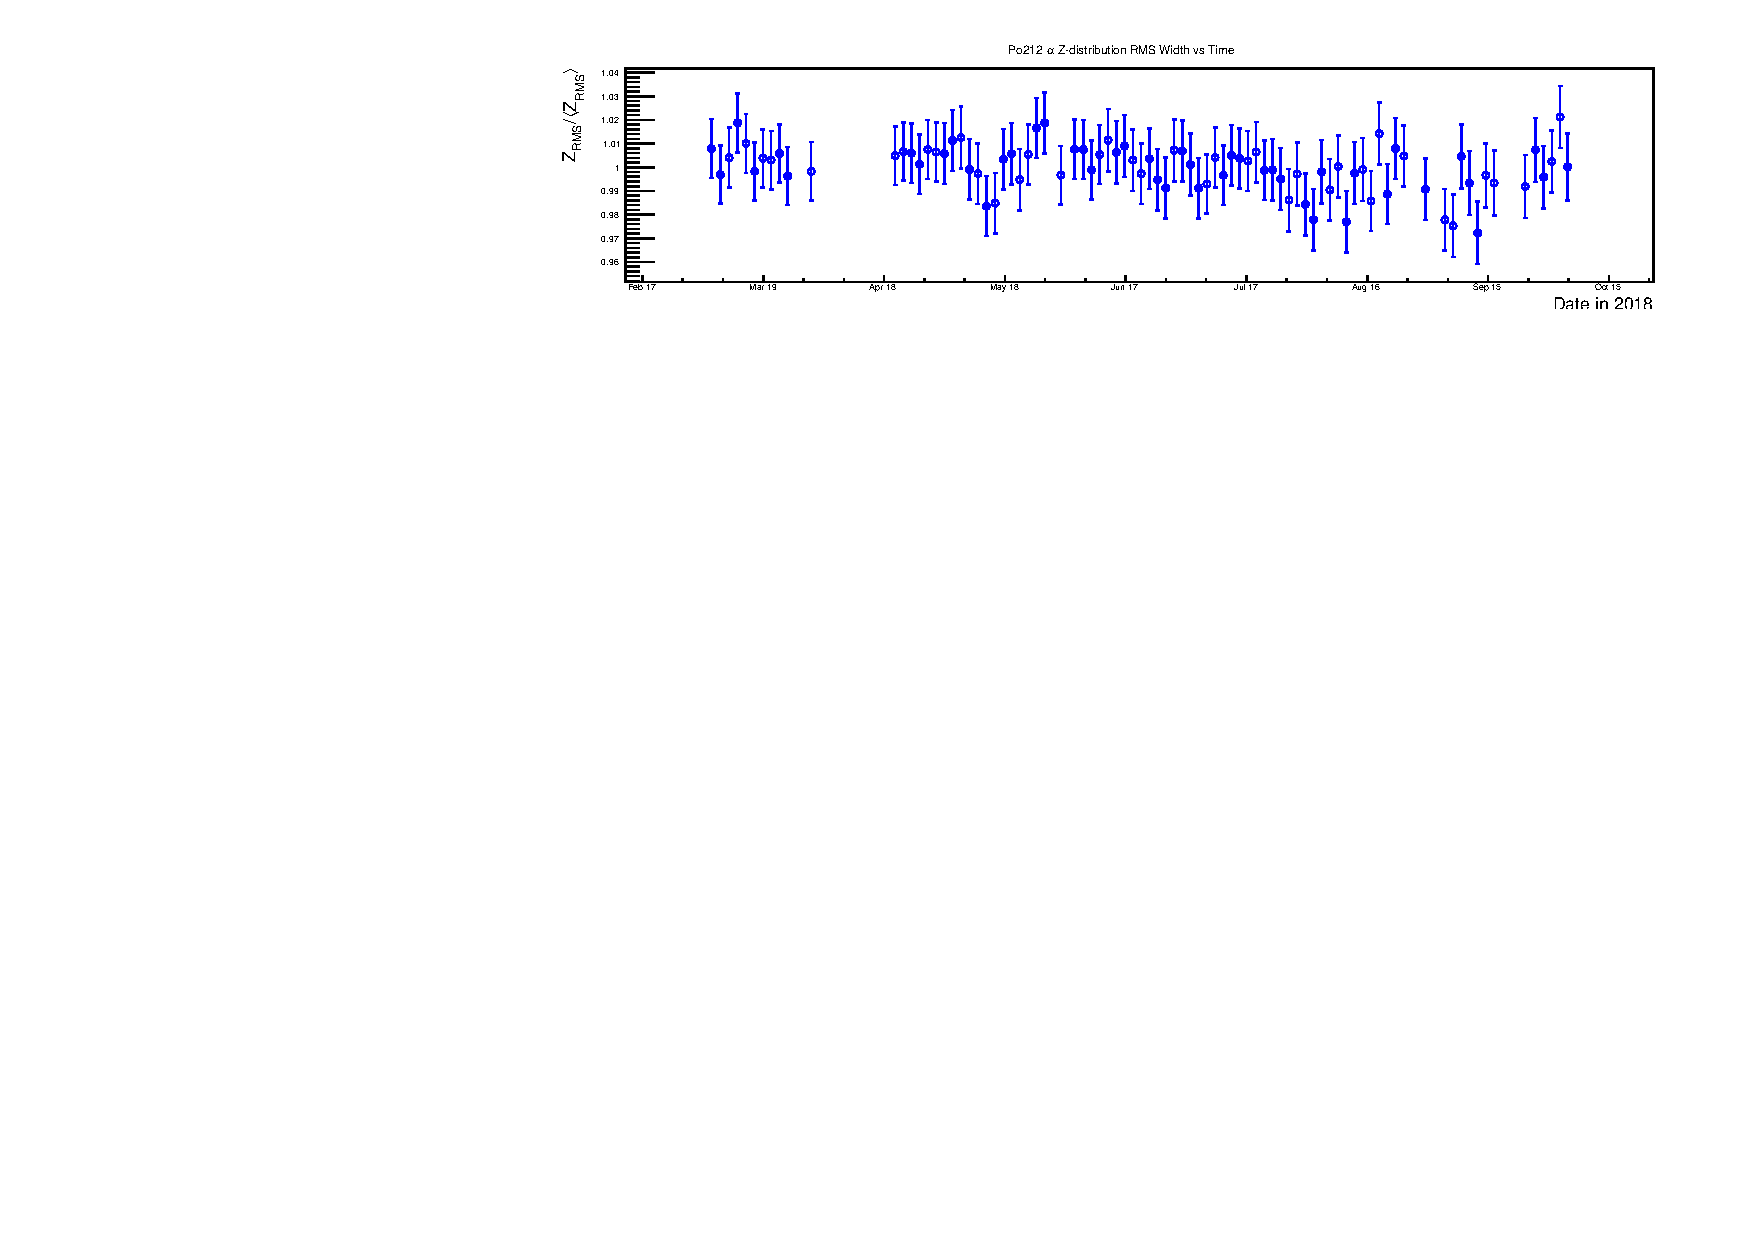
\includegraphics[width=1.05\textwidth]{figures/PubBiPo212ZrmsvsT.pdf}
\caption{\label{fig:ZRMSvsT212}RMS width of Z-distribution of Po-212 alphas versus time. The error bars are the errors assigned by ROOT to the RMS values of the histograms. Values are normalized to the segment error-weighted average to highlight variations. Un-normalized weighted average Z$_{RMS}$ width is 349.0$\pm$0.5~mm and the $\chi^2$/NDF=69.9/60. }
\end{figure}
\begin{figure}[!h]
\centering
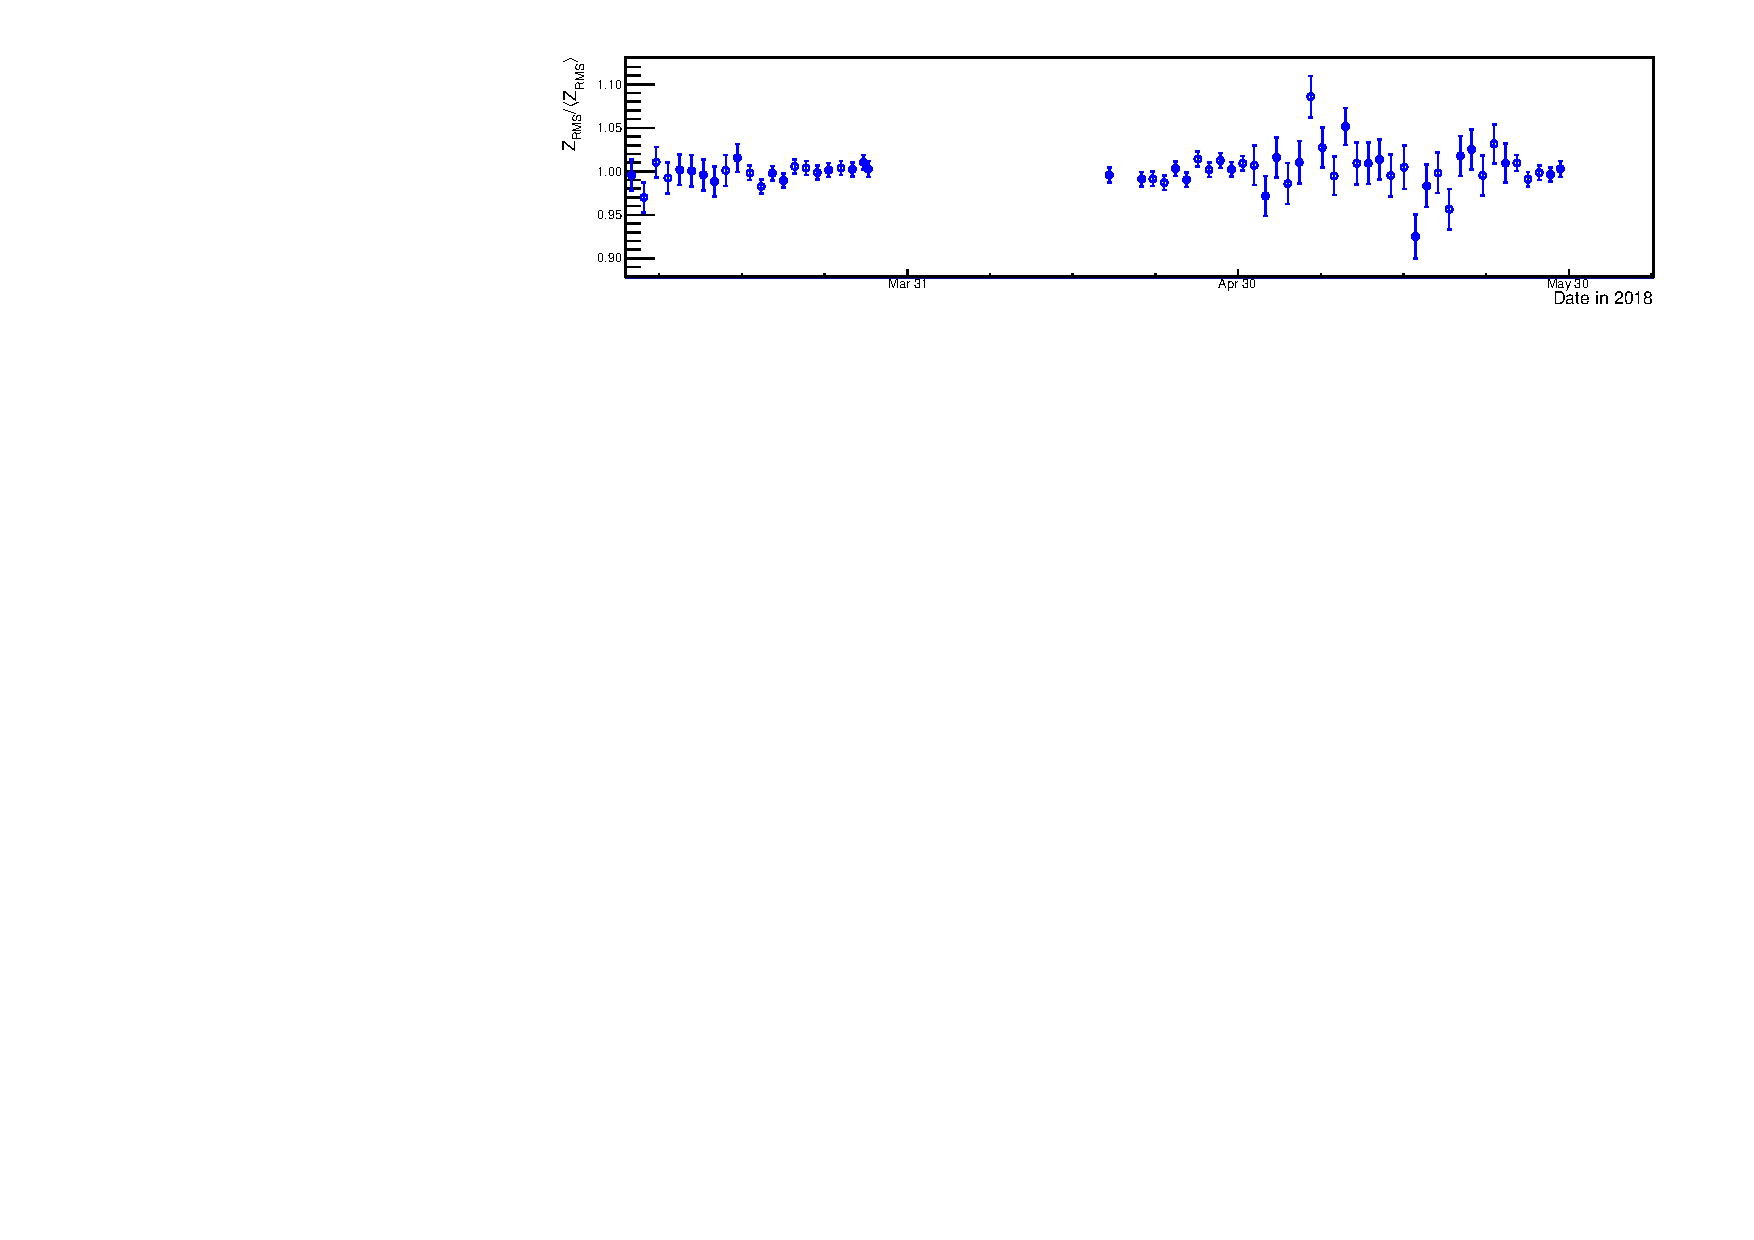
\includegraphics[width=1.05\textwidth]{figures/PubBiPo214ZrmsvsT.pdf}
\caption{\label{fig:ZRMSvsT214}RMS width of Z-distribution of Po-214 alphas versus Time. The error bars are the errors assigned by ROOT to the RMS values of the histograms. Values are normalized to the segment error-weighted average to highlight variations. Un-normalized weighted average Z$_{RMS}$ width is 348.1$\pm$0.7~mm and the $\chi^2$/NDF=56.4/60}
\end{figure}
\newpage
%------------------------------
\subsection{Z-position resolution versus time plots}
\begin{figure}[!h]
\centering
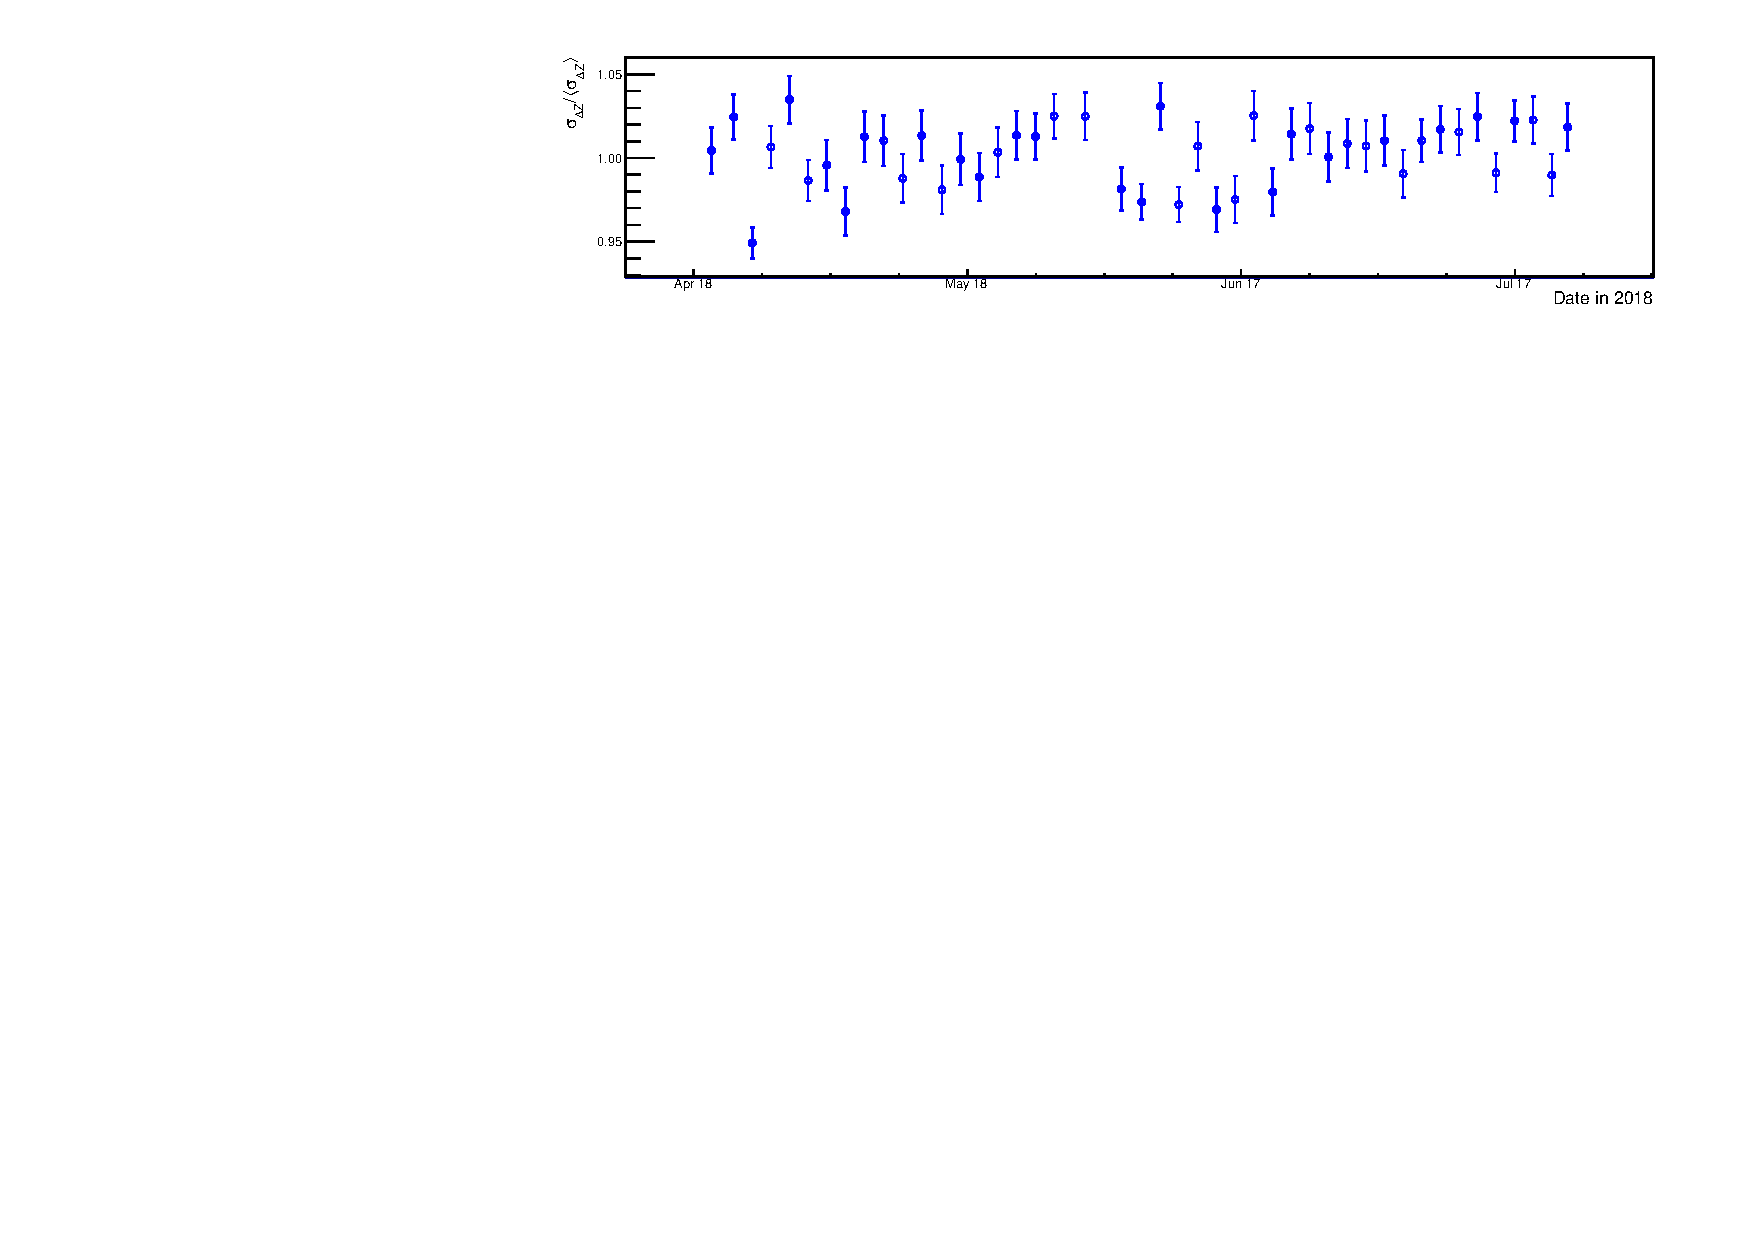
\includegraphics[width=1.05\textwidth]{figures/PubBiPo212ZresvsT.pdf}
\caption{\label{fig:ZresvsT212}Z-position resolution versus time using the beta, alpha from Bi-212, Po-212. The values are the 1$\sigma$ widths of a Gaussian fits to the alpha minus beta Z-distance distributions and the error bars are the error on these values from the fit. Values are normalized to the segment error-weighted average to highlight variations. Un-normalized weighted average $\Delta$Z width is 45.84$\pm$0.11~mm and the $\chi^2$/NDF=164/60.}
\end{figure}
\begin{figure}[!h]
\centering
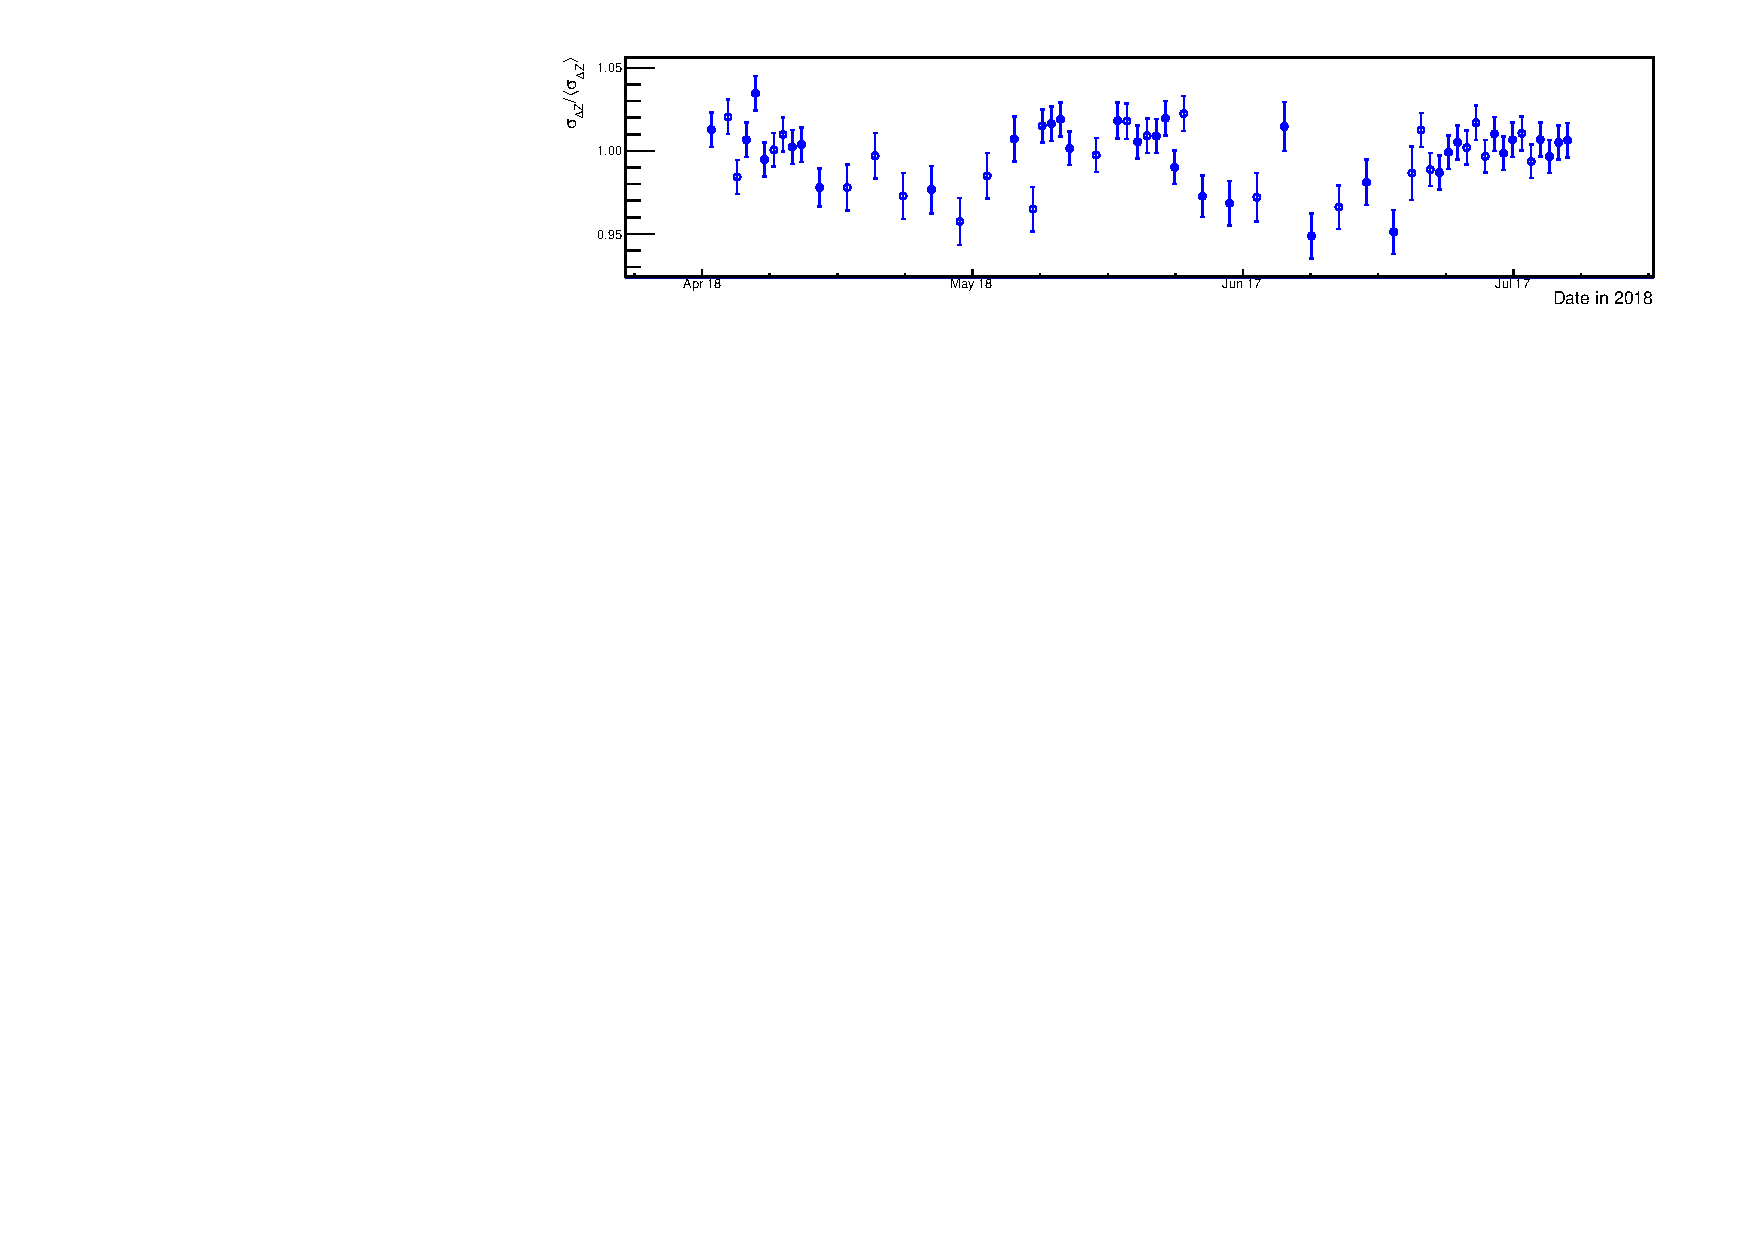
\includegraphics[width=1.05\textwidth]{figures/PubBiPo214ZresvsT.pdf}
\caption{\label{fig:ZresvsT214}Z-position resolution versus time using the beta, alpha from Bi-214, Po-214. The values are the 1$\sigma$ widths of a Gaussian fits to the alpha minus beta Z-distance distributions and the error bars are the error on these values from the fit. Values are normalized to the segment error-weighted average to highlight variations.Un-normalized weighted average $\Delta$Z width is 55.75$\pm$0.13~mm and the $\chi^2$/NDF=164/60. Presumably, the larger width is due to the presence of higher energy gammas accompanying the Po-214 beta decay. Reactor on periods can be seen to have larger errors due to increased accidental backgrounds.}
\end{figure}
\newpage
%------------------------------
\subsection{Z-position distribution mean versus segment plots}
\begin{figure}[!h]
\centering
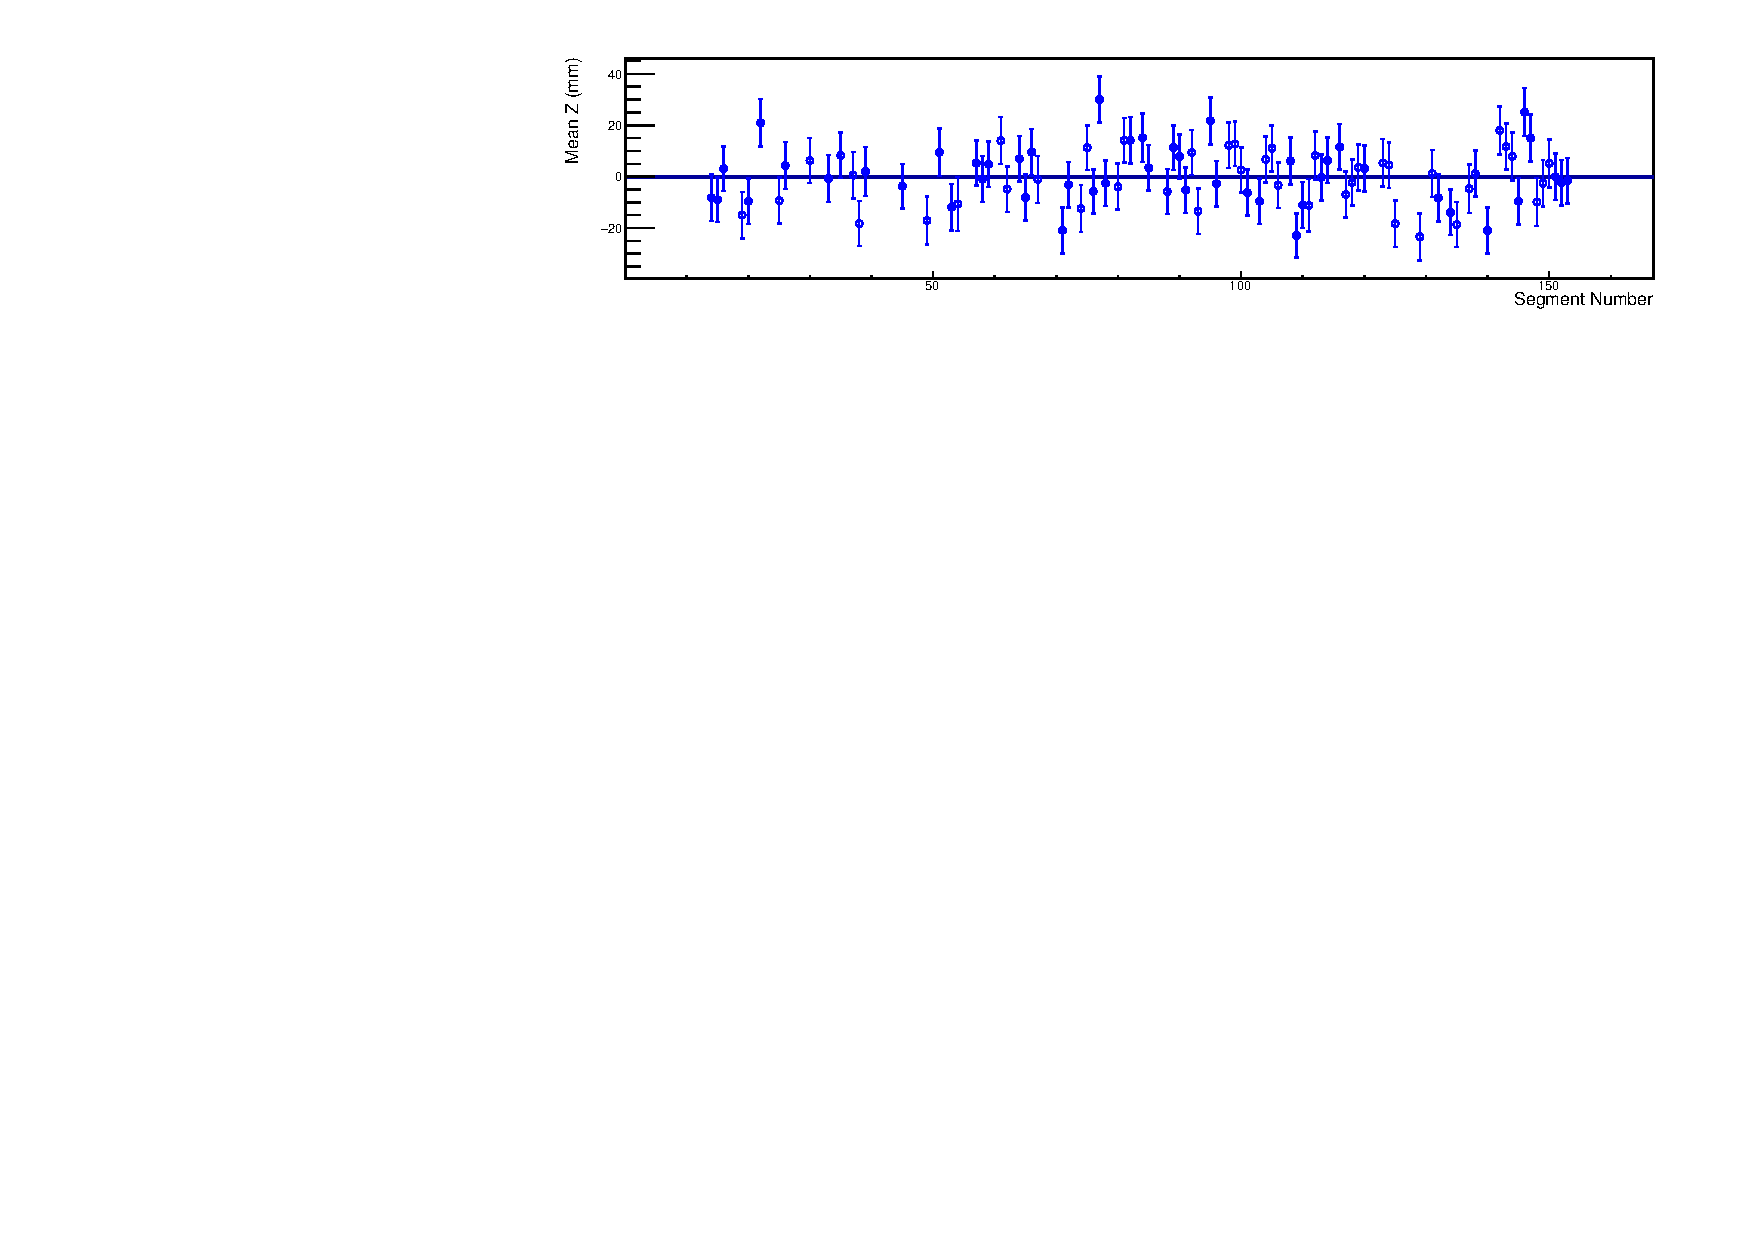
\includegraphics[width=1.05\textwidth]{figures/PubBiPo212meanZvsCell.pdf}
\caption{\label{fig:meanZvsCell212}Mean of Z-position distribution of Po-212 alphas versus segment. The values are distributions averages and the error bars are the RMS of the distribution. Values are normalized to the segment error-weighted average to highlight variations. Un-normalized weighted average mean Z-position is 3.3$\pm$0.9~mm and $\chi^2$/NDF=489/122. Segment 8 has been seen to be problematic.}
\end{figure}
\begin{figure}[!h]
\centering
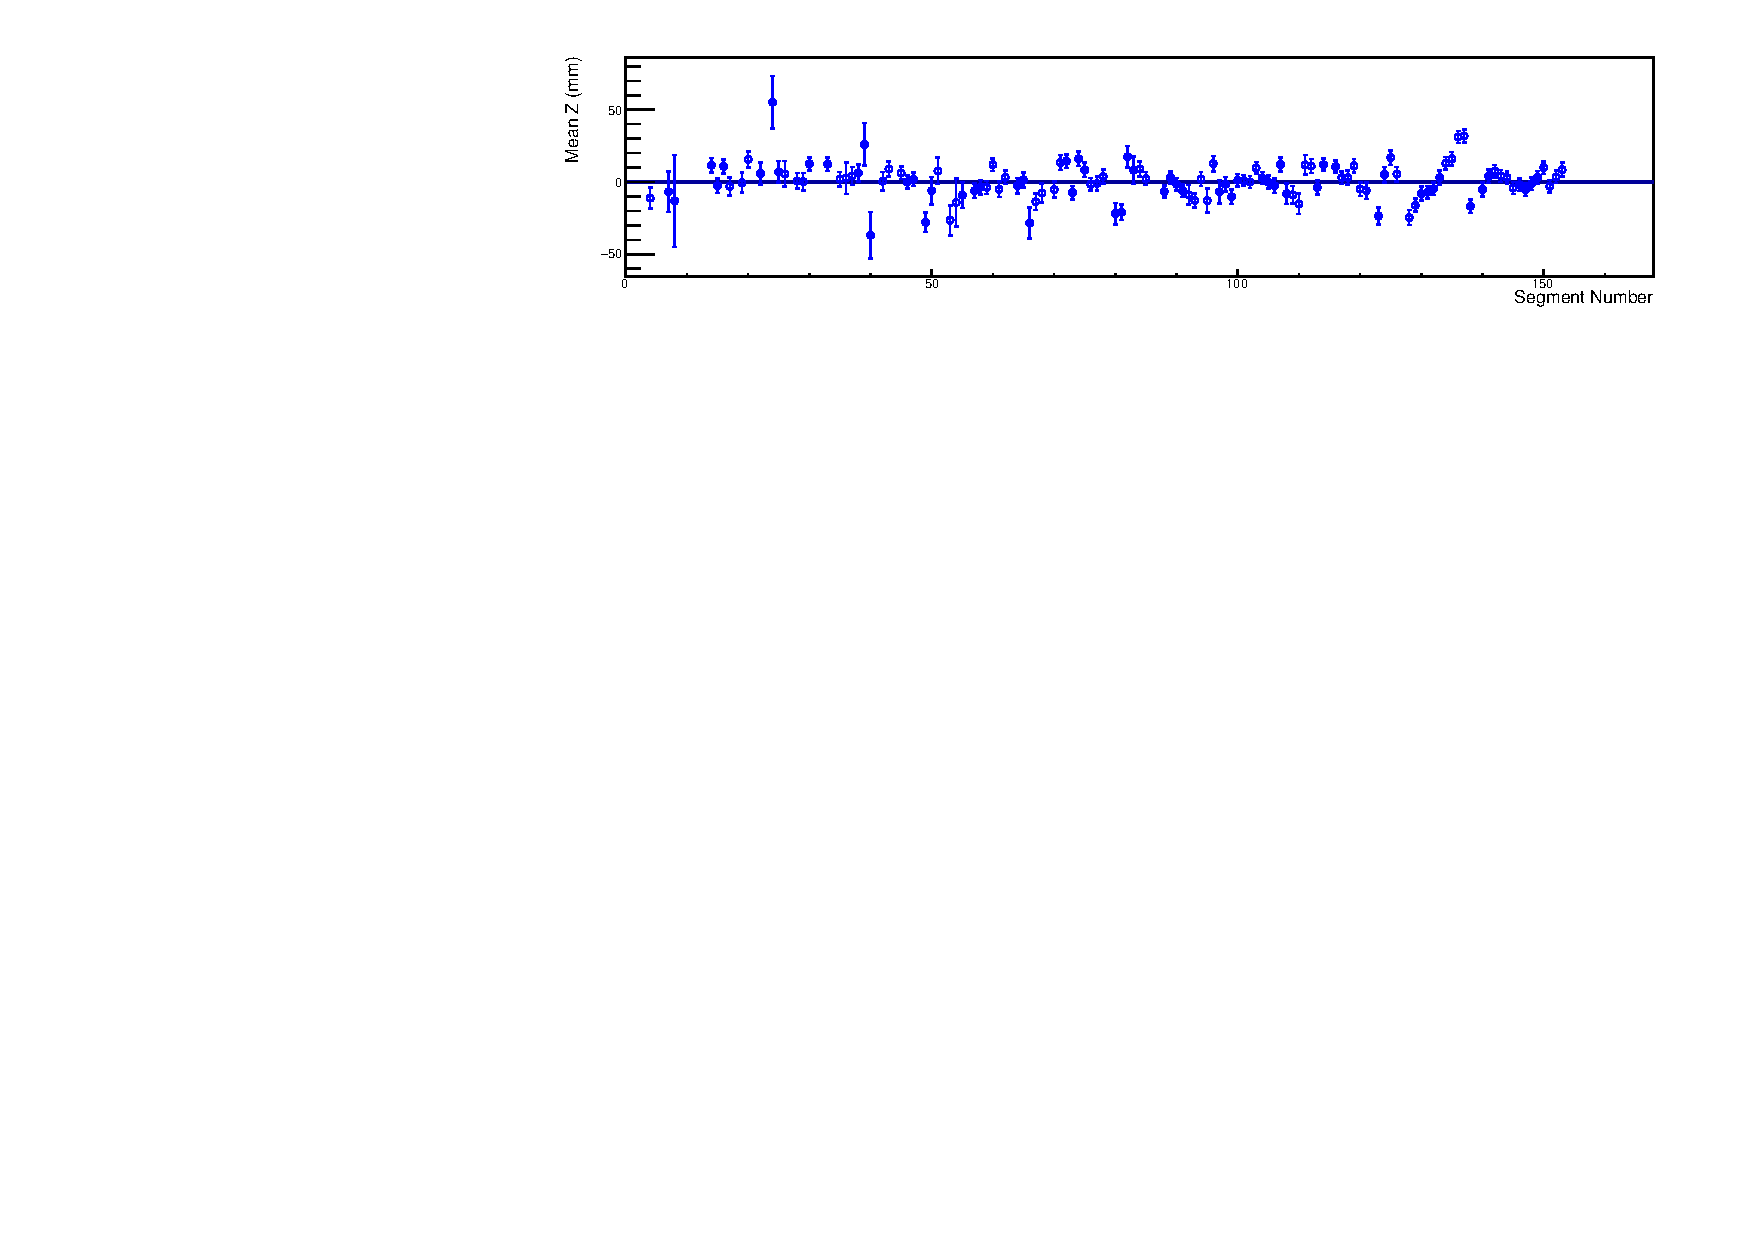
\includegraphics[width=1.05\textwidth]{figures/PubBiPo214meanZvsCell.pdf}
\caption{\label{fig:meanZvsCell214}Mean of Z-position distribution of Po-214 alphas versus segment. The values are distributions averages and the error bars are the RMS of the distribution. Values are normalized to the segment error-weighted average to highlight variations. Un-normalized weighted average mean Z-position is 2.5$\pm$0.9~mm and $\chi^2$/NDF=171/122.}
\end{figure}
\newpage
%------------------------------
\subsection{Whole detector alpha energy spectrum}
\begin{figure}[!h]
\centering
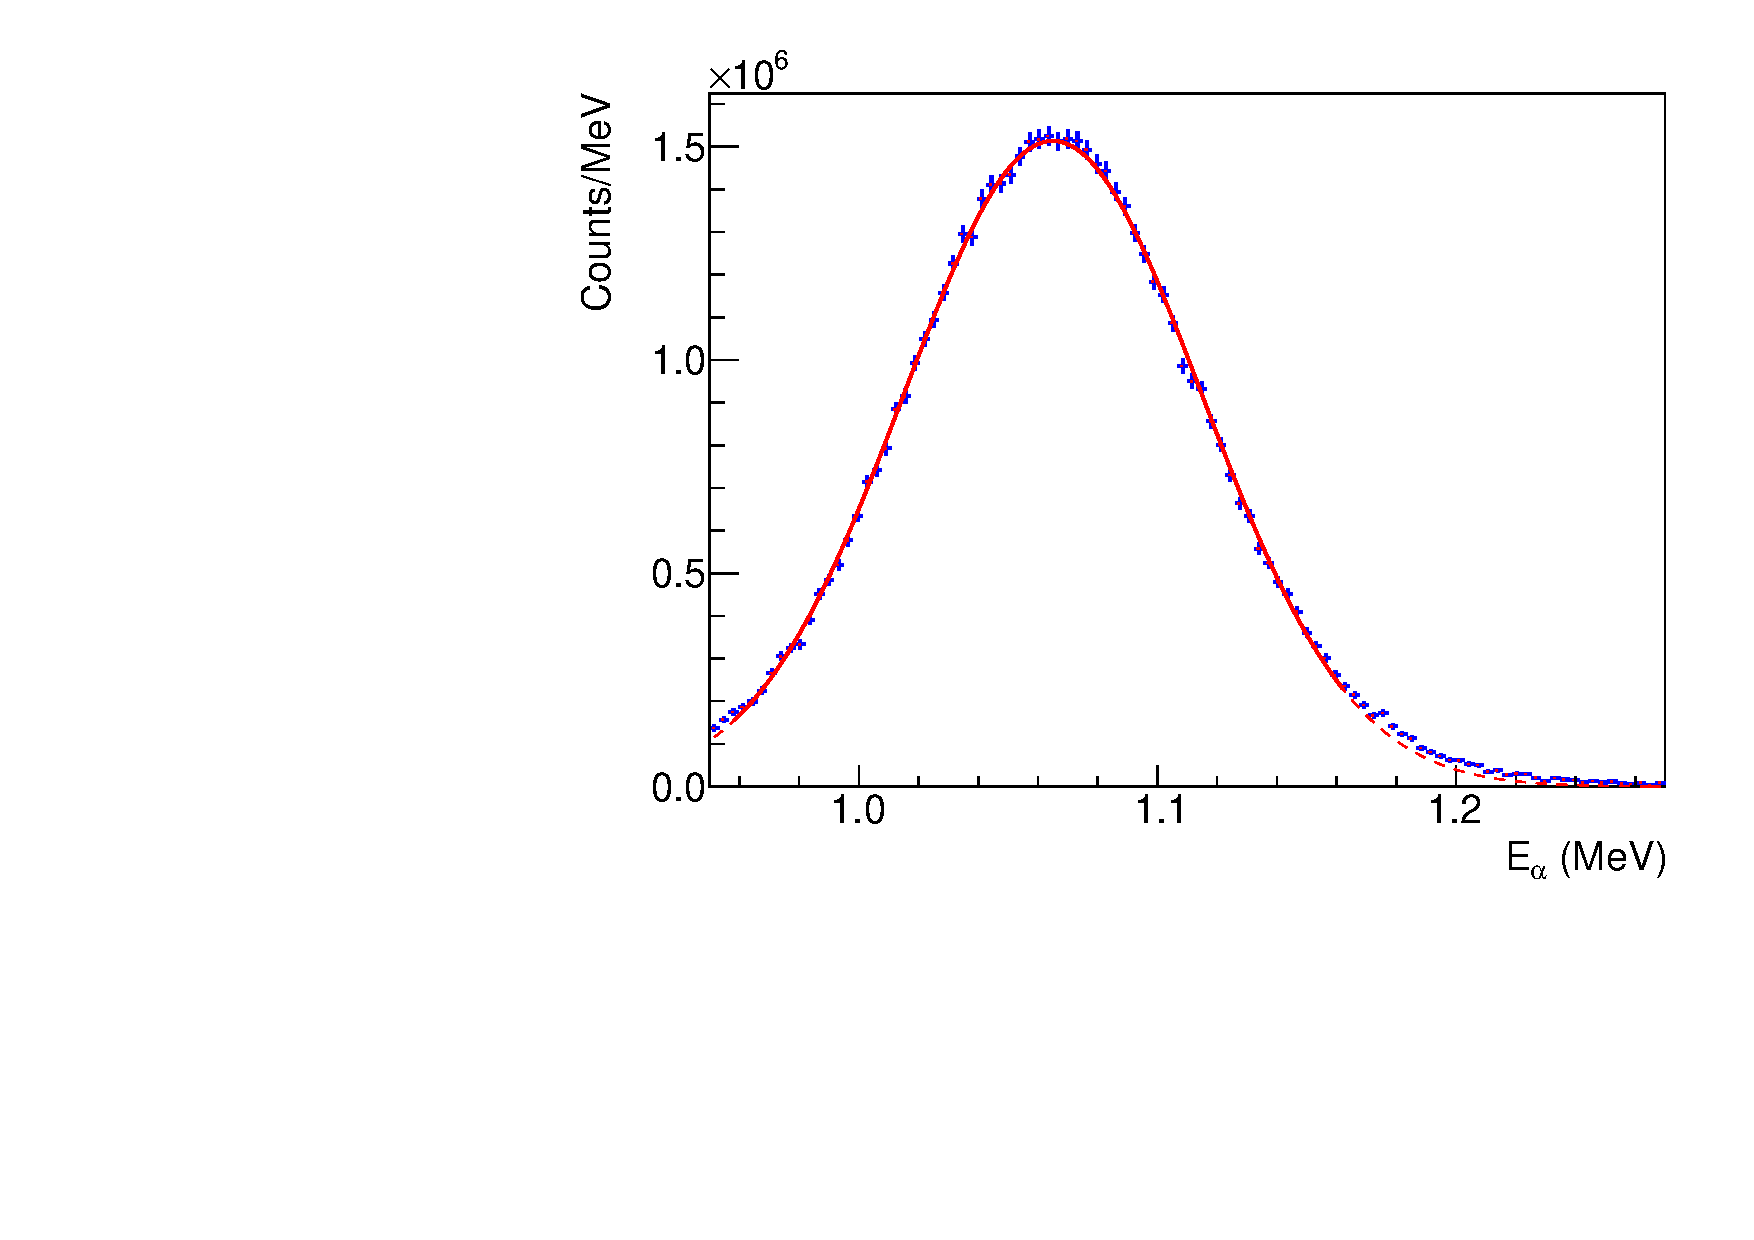
\includegraphics[width=0.66\textwidth]{figures/PubBiPo212AlphaE.pdf}
\caption{\label{fig:AlphaE212}Whole detector Po-212 alpha energy spectrum. The mean of this fit is 1.08757$\pm$0.00015~MeV and the width is 0.05000$\pm$0.00013~MeV. This is an essentially mono-energetic alpha with 8.785~MeV of energy.}
\end{figure}
\begin{figure}[!h]
\centering
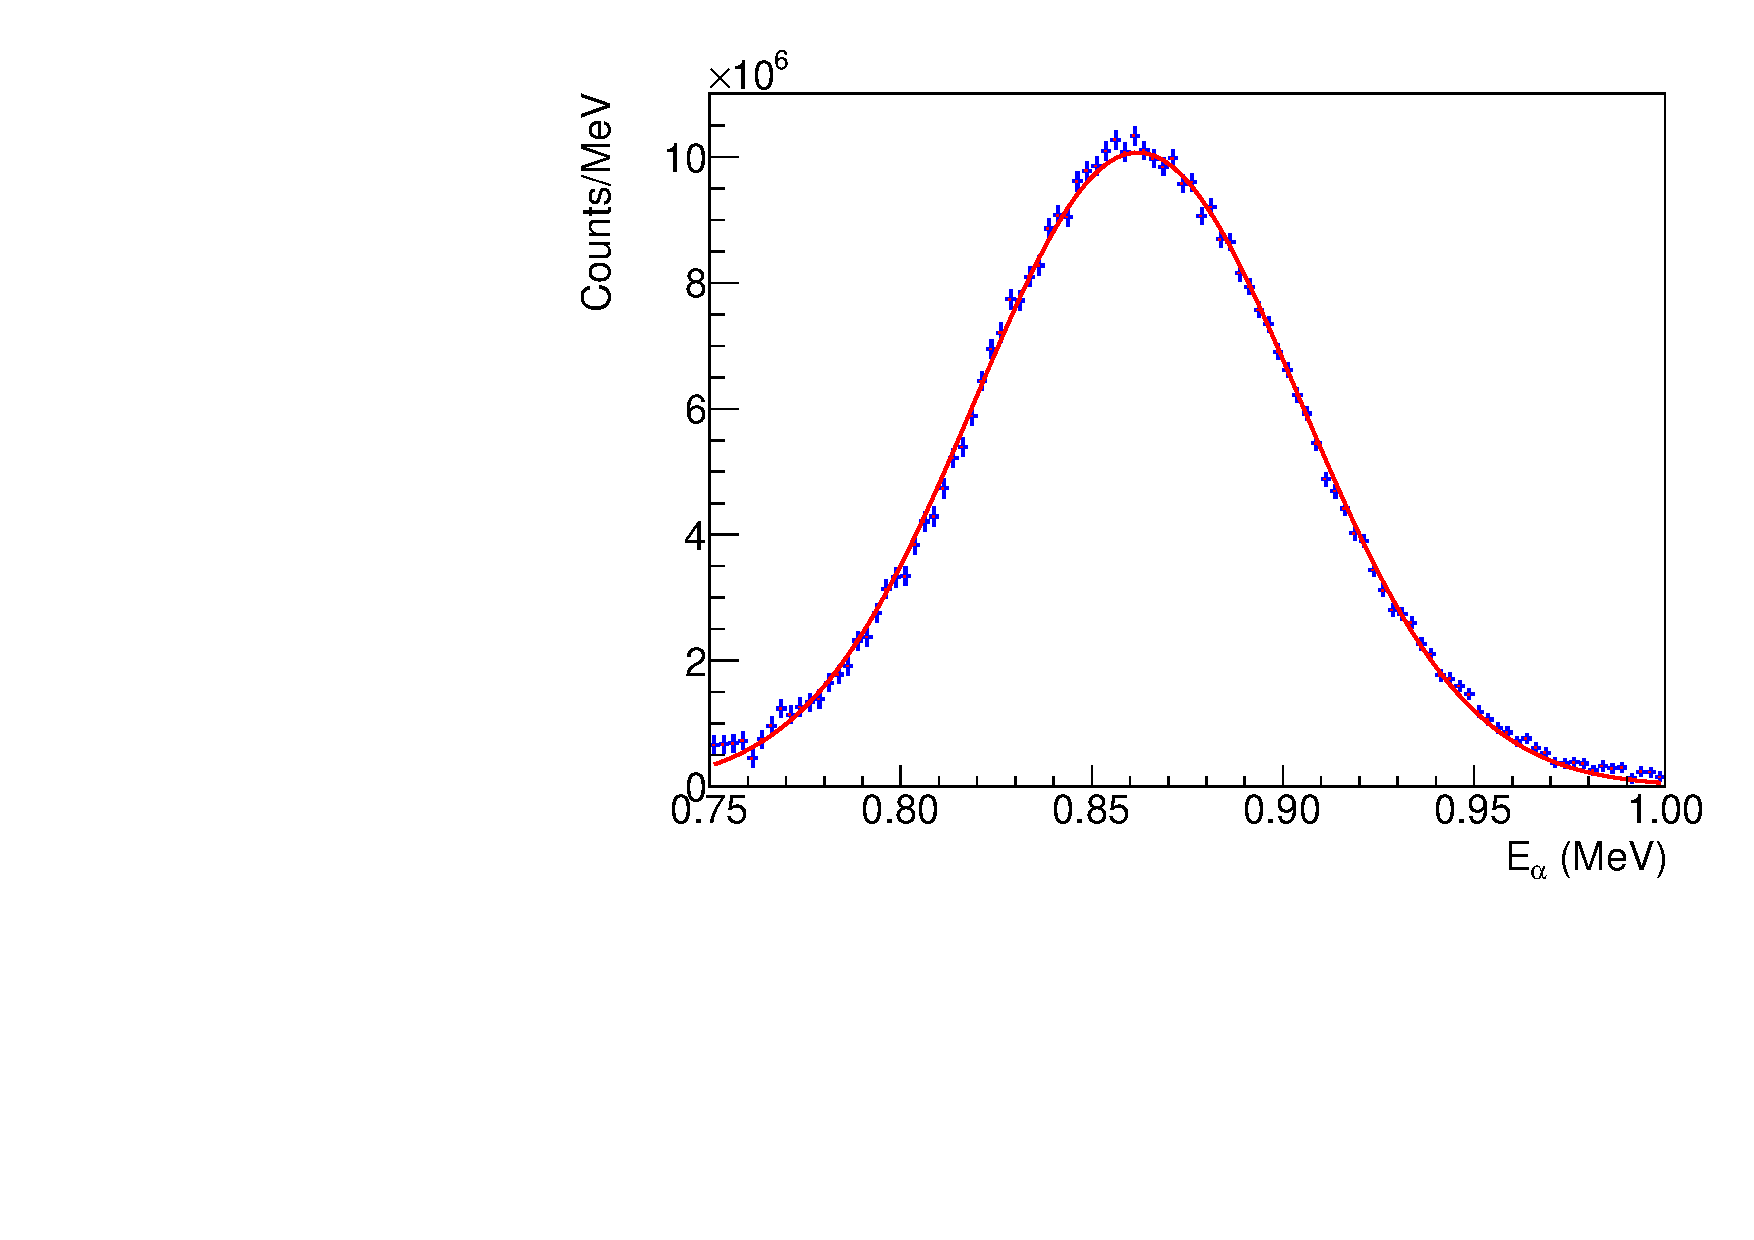
\includegraphics[width=0.66\textwidth]{figures/PubBiPo214AlphaE.pdf}
\caption{\label{fig:AlphaE214}Whole detector Po-214 alpha energy spectrum. The mean of this fit is 0.86200$\pm$0.00015~MeV and the width is 0.04272$\pm$0.00014~MeV. This is an essentially mono-energetic alpha with 7.687~MeV of energy.}
\end{figure}
\newpage
%------------------------------
\subsection{Whole detector beta energy spectrum}
\begin{figure}[!h]
\centering
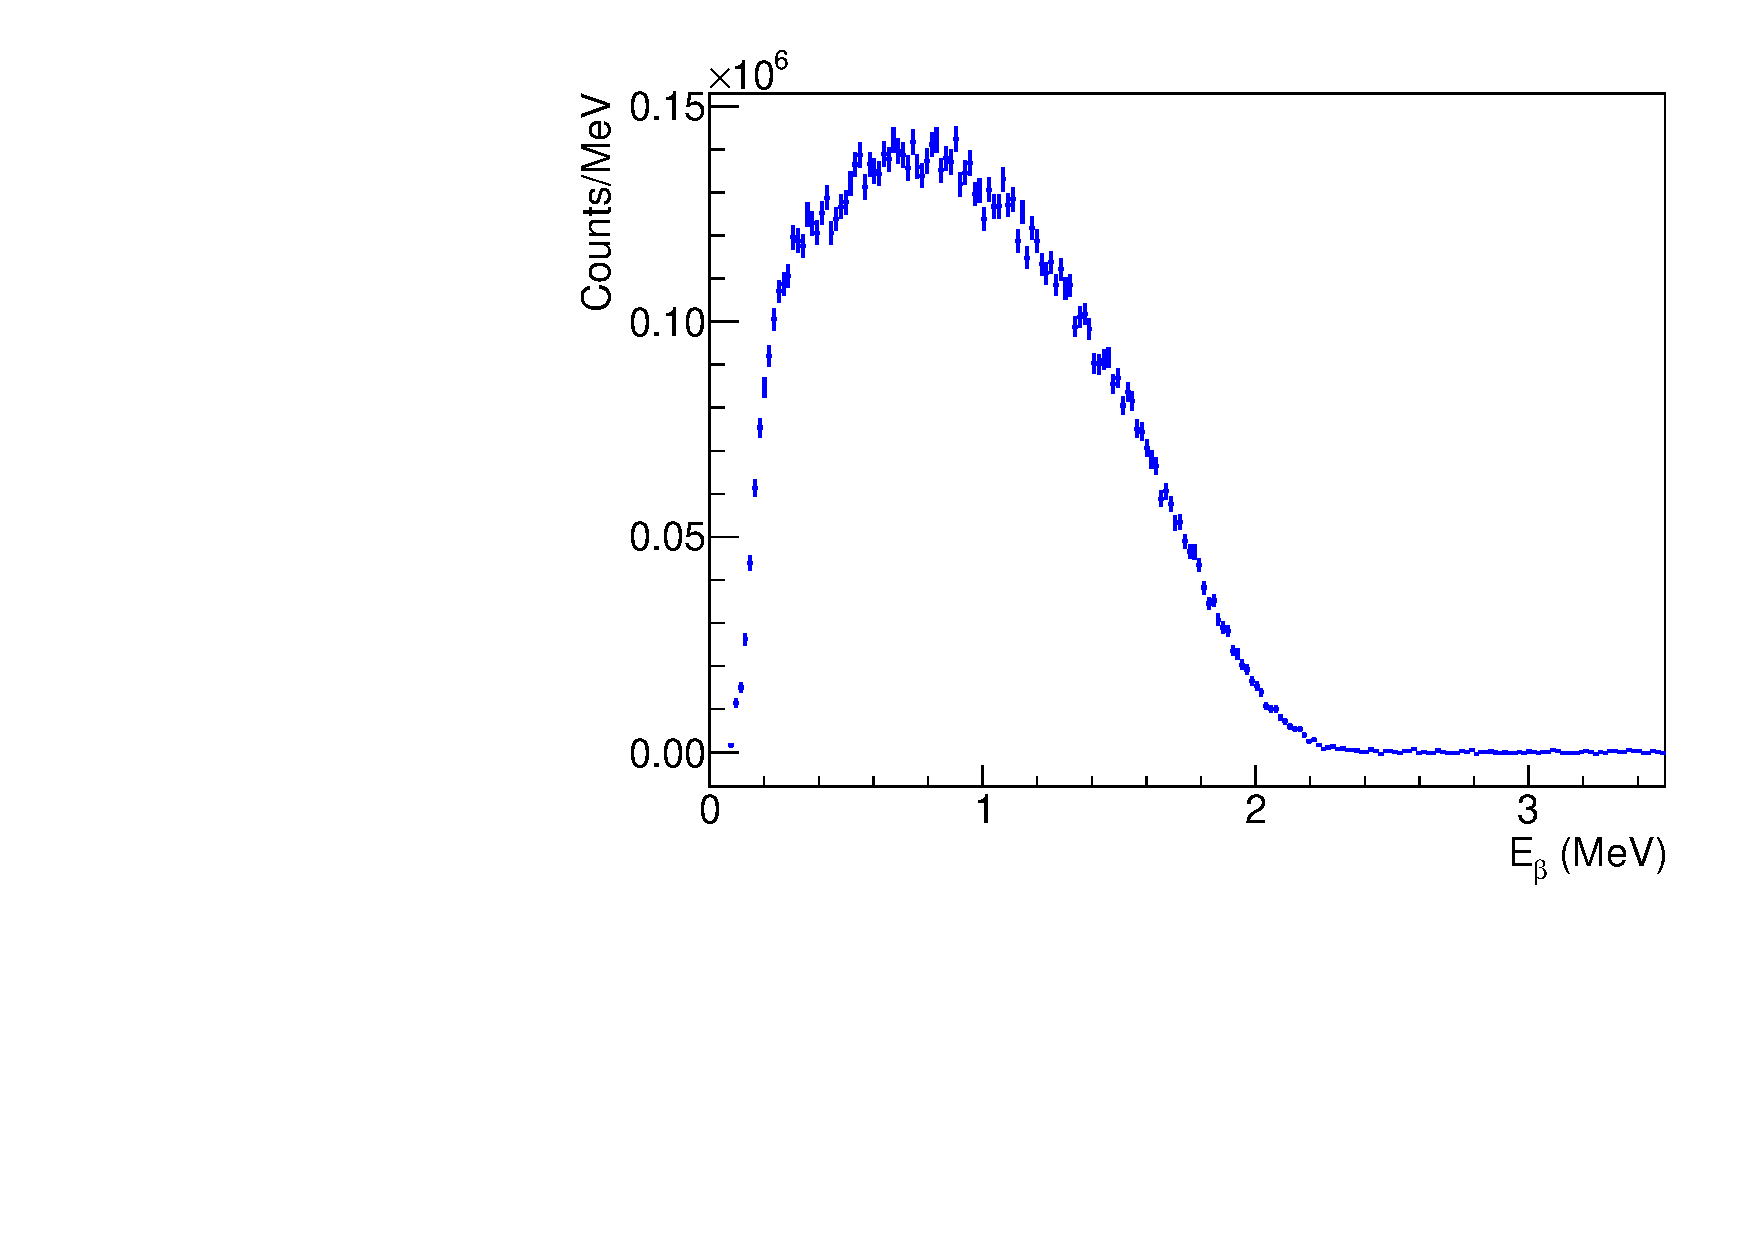
\includegraphics[width=0.7\textwidth]{figures/PubBiPo212BetaE.pdf}
\caption{\label{fig:BetaE212}Whole detector Bi-212 beta energy spectrum. The beta endpoint for this decay is 2.252(2)~MeV.}
\end{figure}
\begin{figure}[!h]
\centering
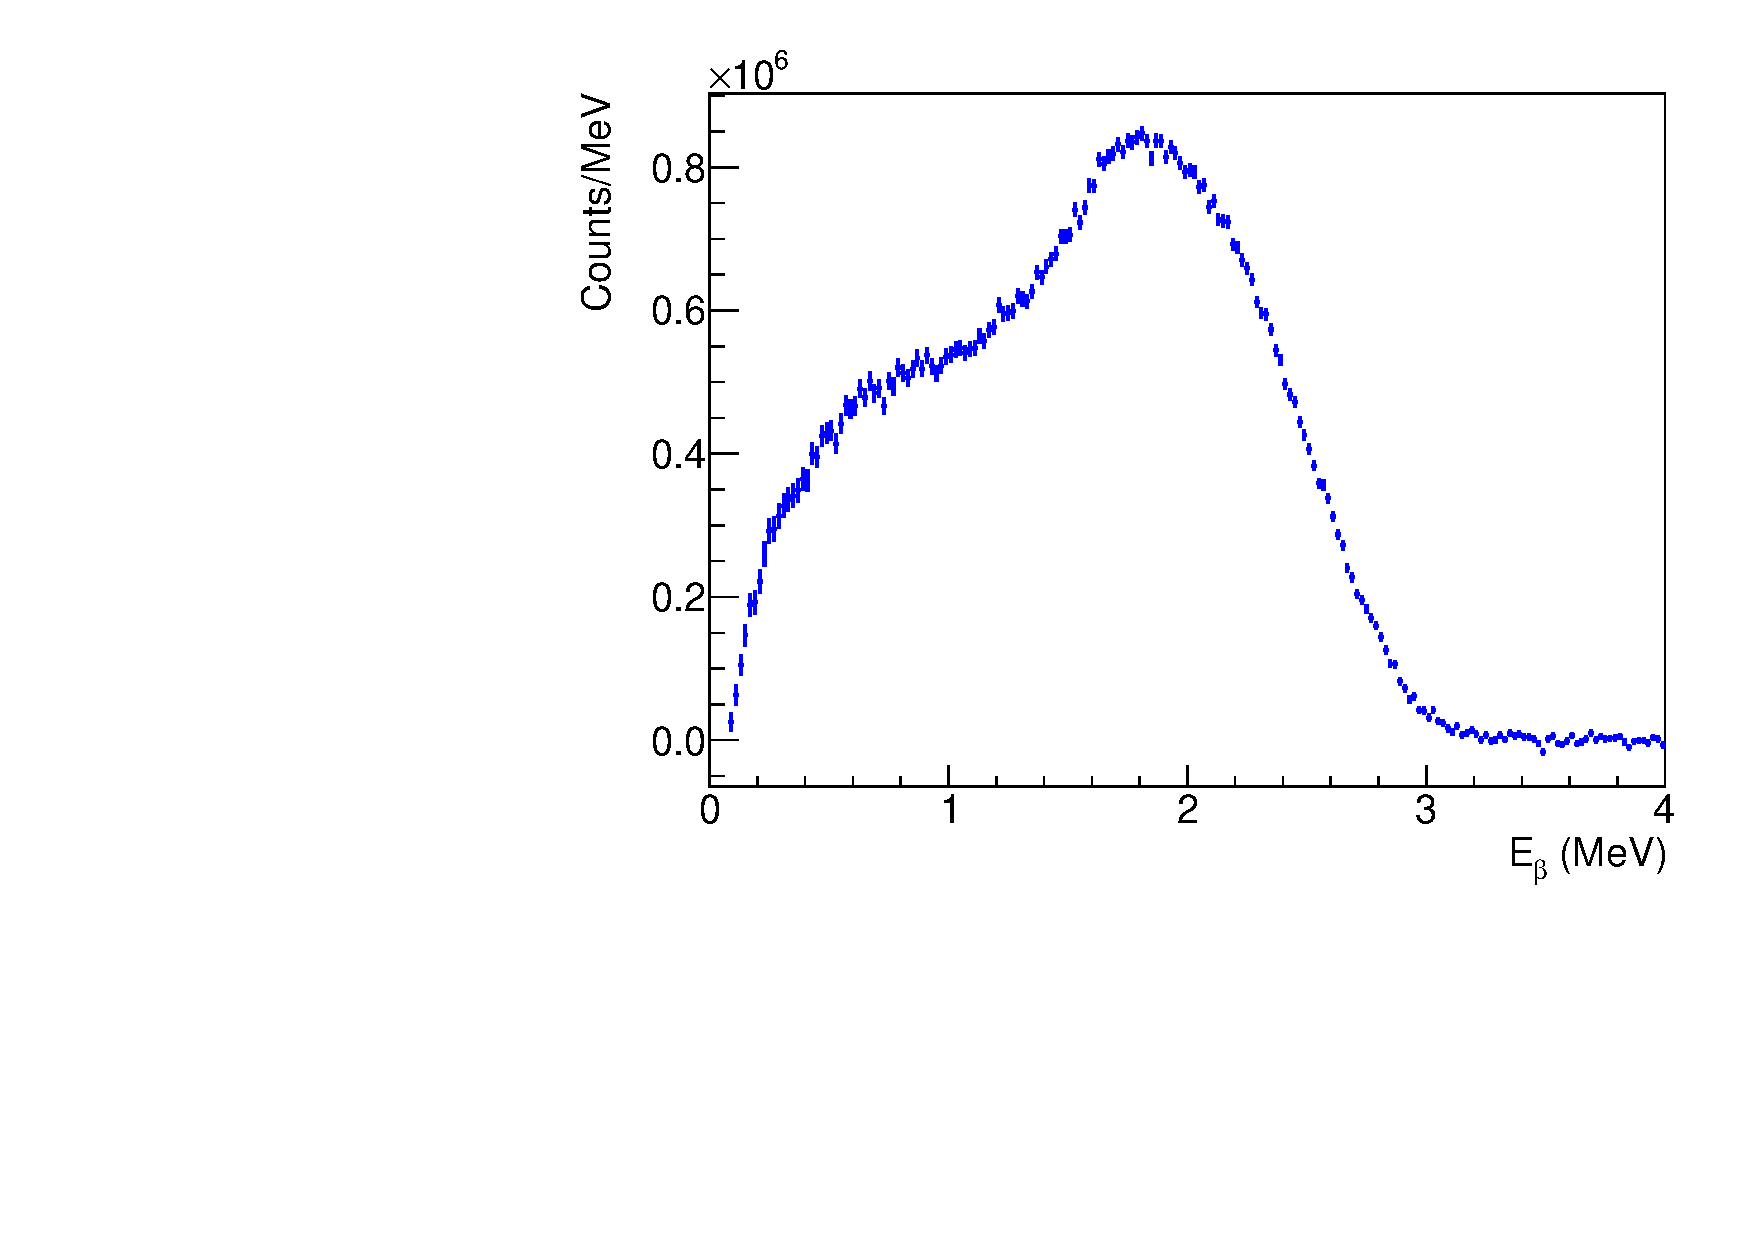
\includegraphics[width=0.7\textwidth]{figures/PubBiPo214BetaE.pdf}
\caption{\label{fig:BetaE214}Whole detector Bi-214 beta energy spectrum. The beta endpoint for this decay is 3.269(11)~MeV.}
\end{figure}
\newpage
%------------------------------
\subsection{Whole detector Po alpha Z-position distribution}
\begin{figure}[!h]
\centering
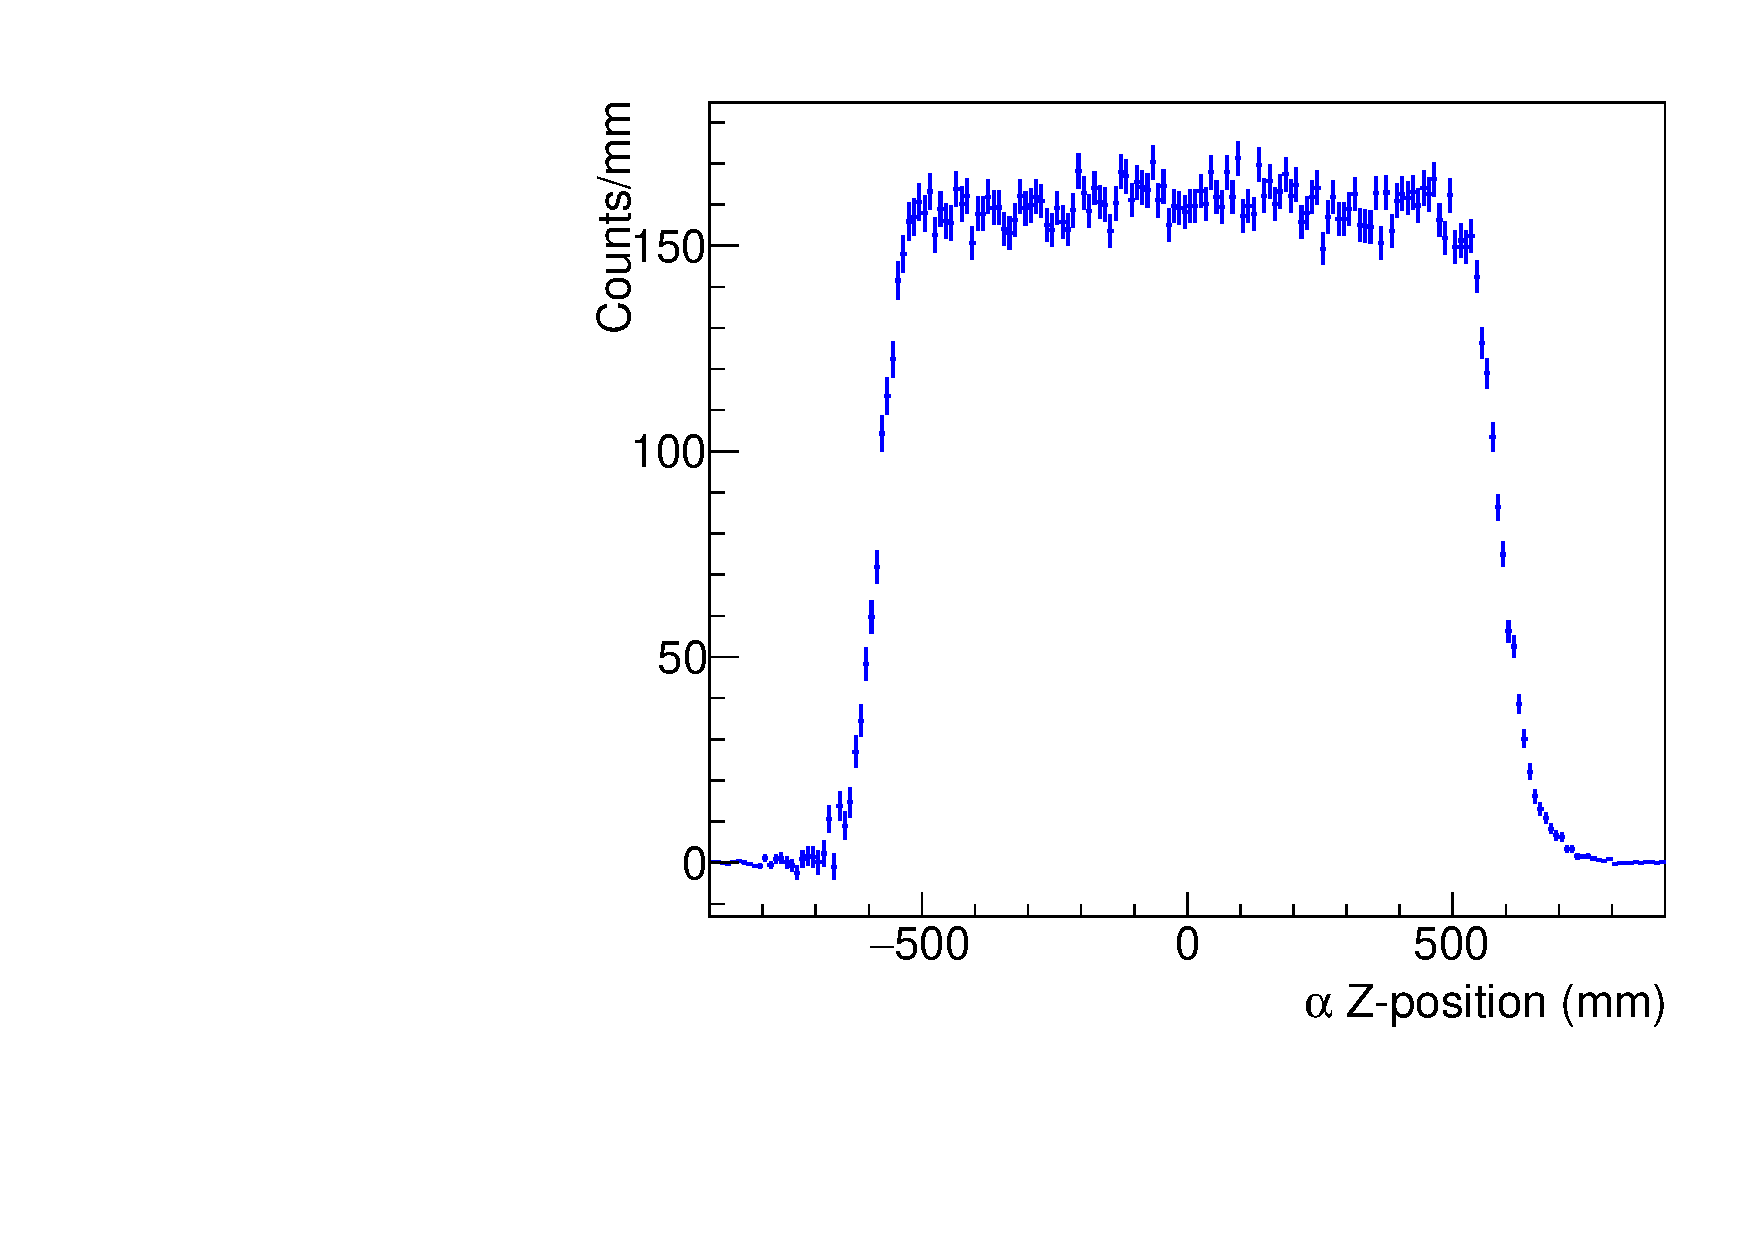
\includegraphics[width=0.6\textwidth]{figures/PubBiPo212Zdistribution.pdf}
\caption{\label{fig:Z212}Whole detector Po-212 alpha Z-position distribution.}
\end{figure}
\begin{figure}[!h]
\centering
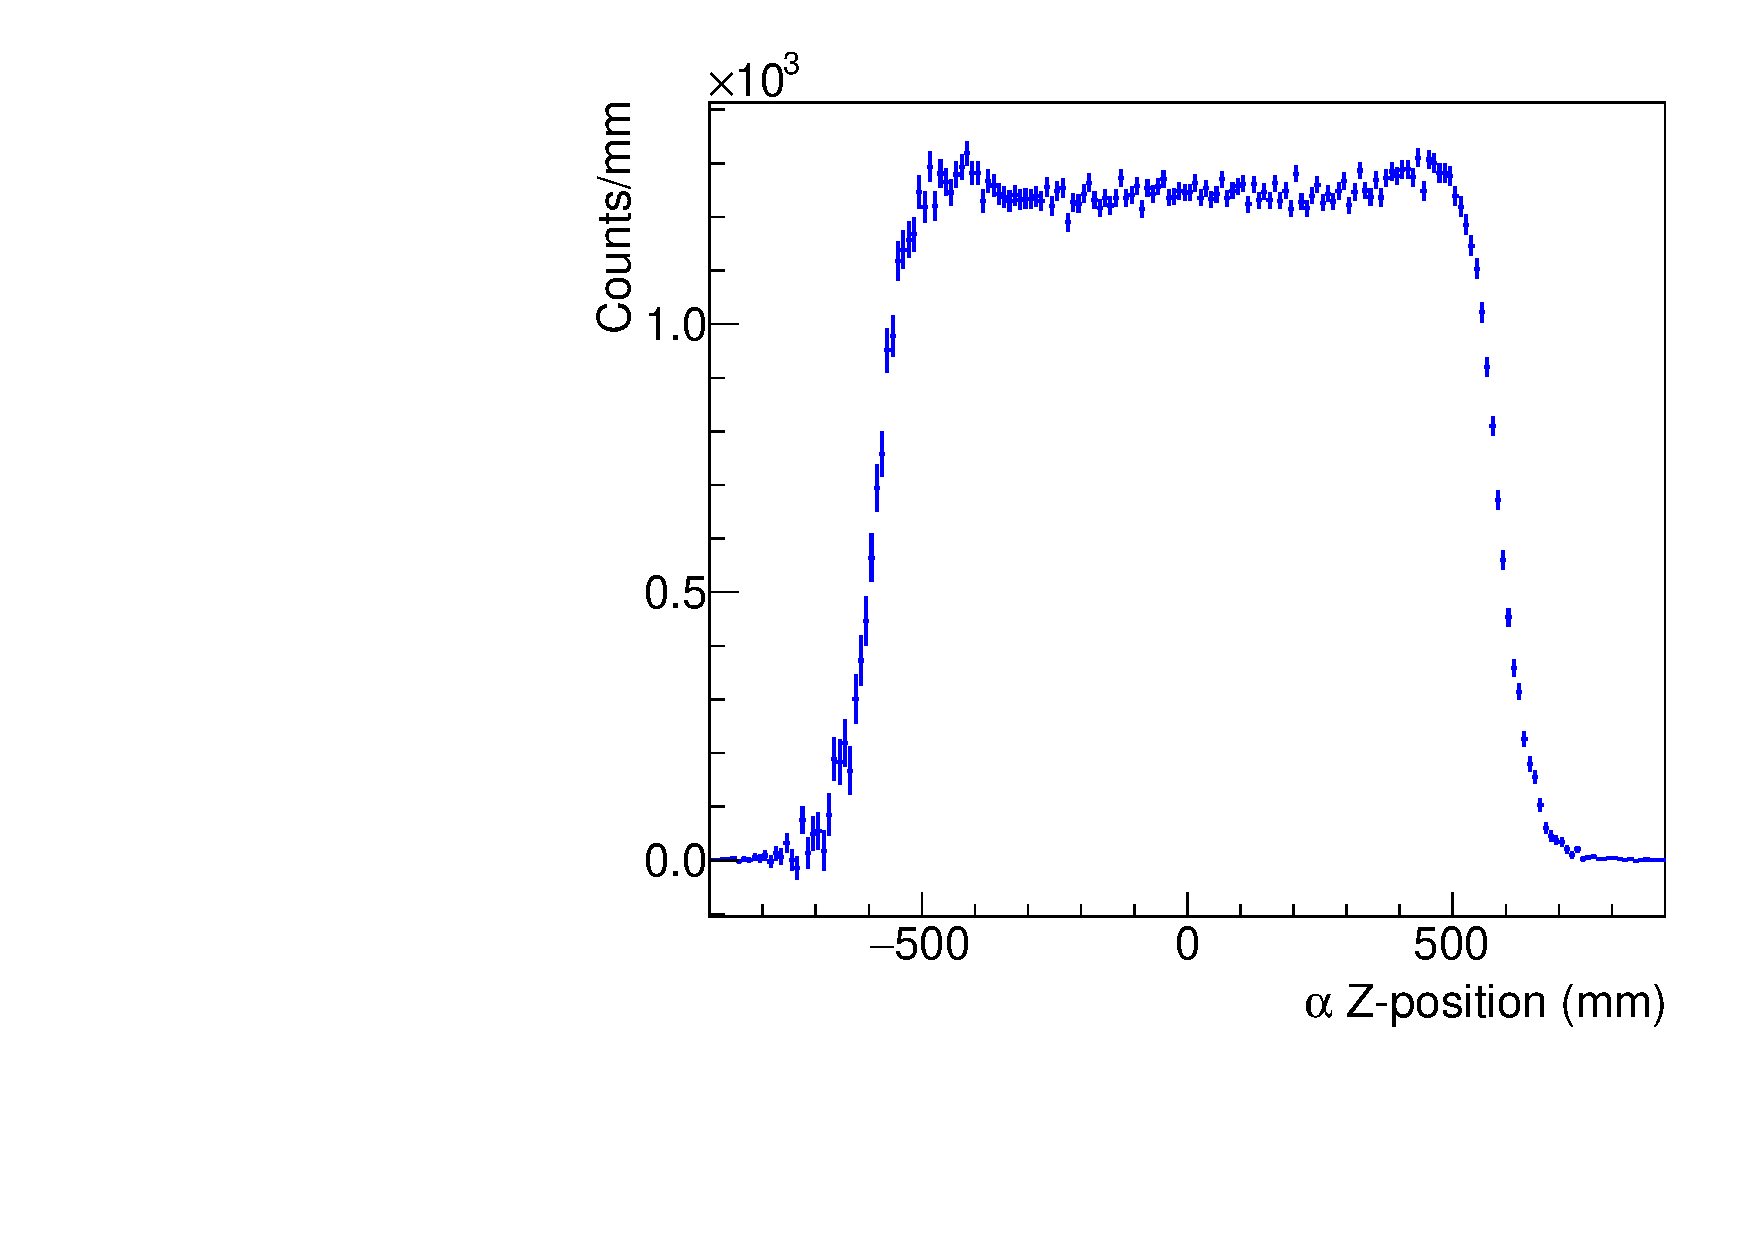
\includegraphics[width=0.6\textwidth]{figures/PubBiPo214Zdistribution.pdf}
\caption{\label{fig:Z214}Whole detector Po-214 alpha Z-position distribution.}
\end{figure}
\newpage
%------------------------------
\subsection{Whole detector BiPo dZ distribution}
\begin{figure}[!h]
\centering
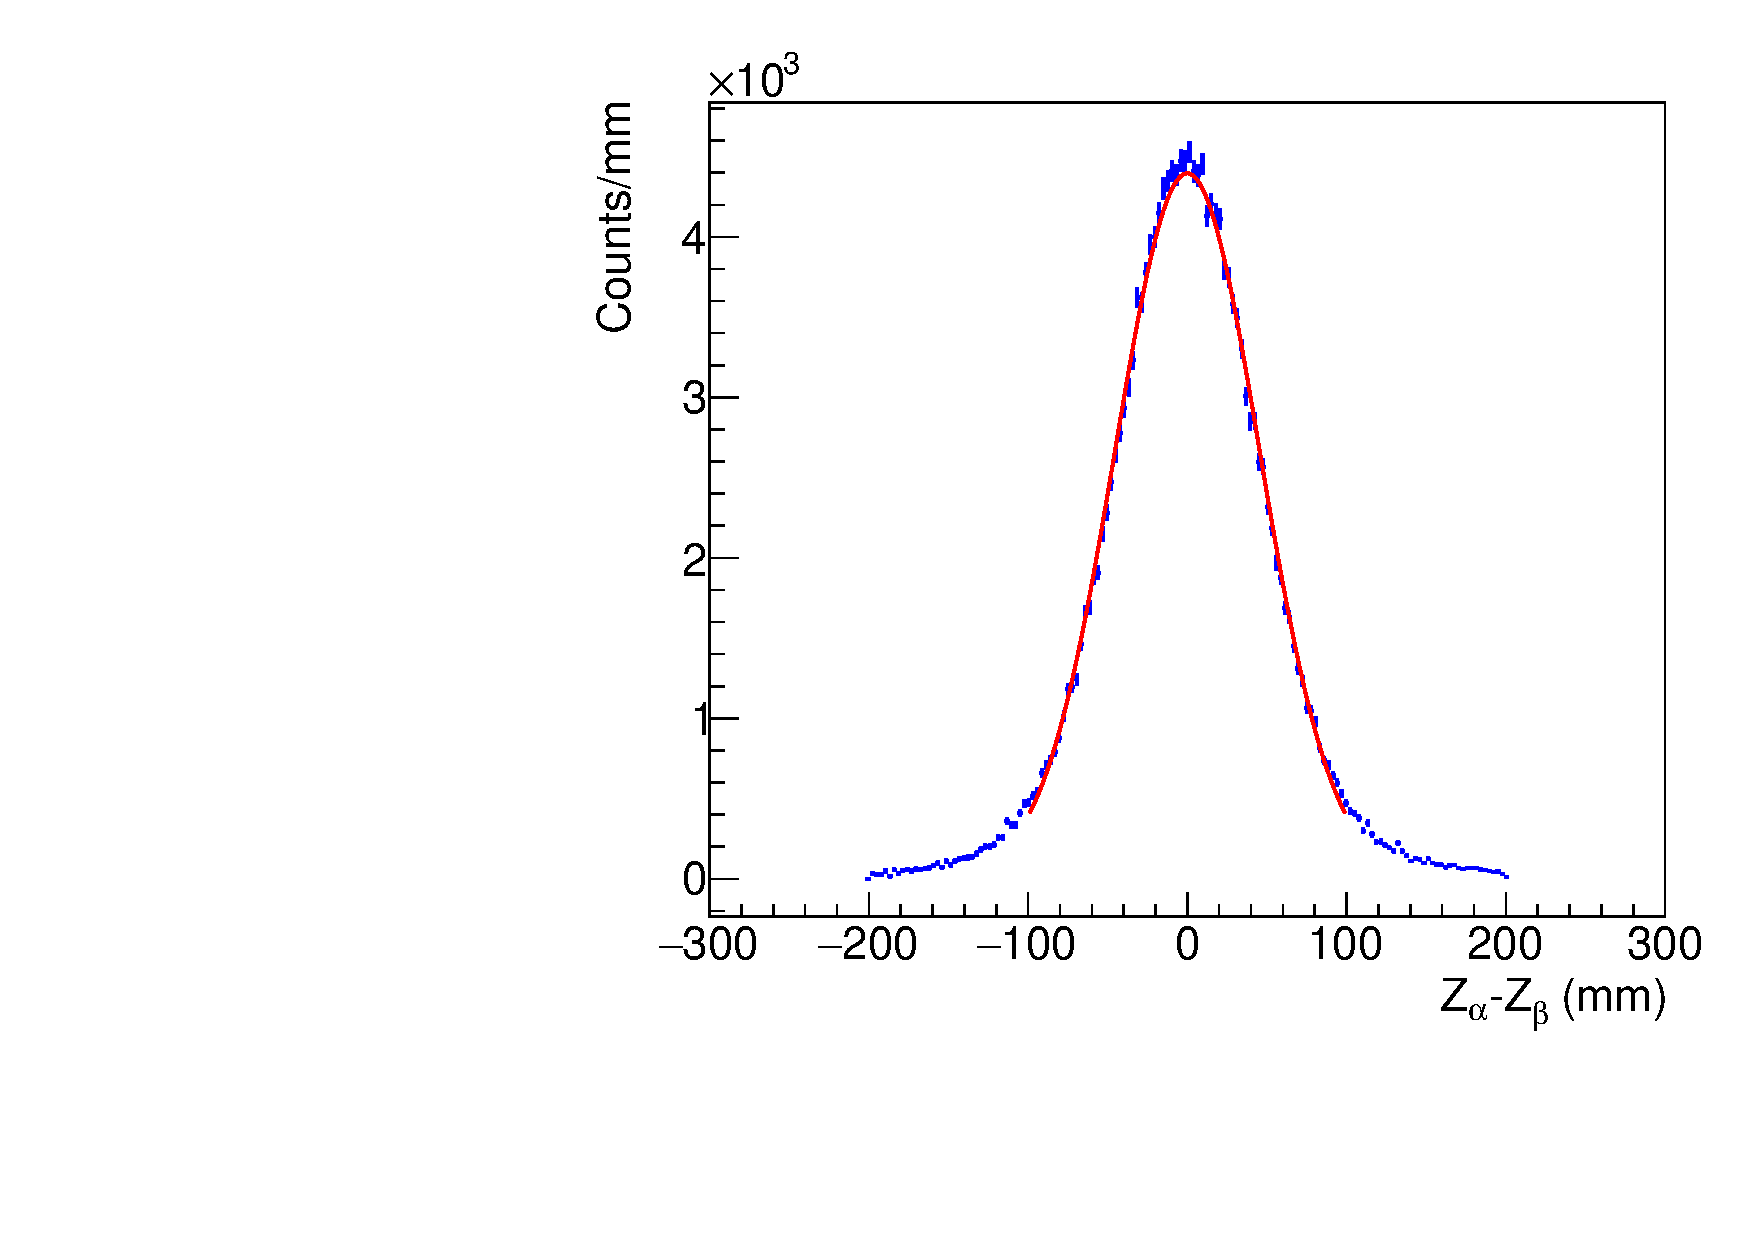
\includegraphics[width=0.6\textwidth]{figures/PubBiPo212dZ.pdf}
\caption{\label{fig:Z212}Whole detector distribution of Po-212 alpha, beta correlation distance $\Delta$Z. The width of this distribution is 46.06$\pm$0.13~mm.}
\end{figure}
\begin{figure}[!h]
\centering
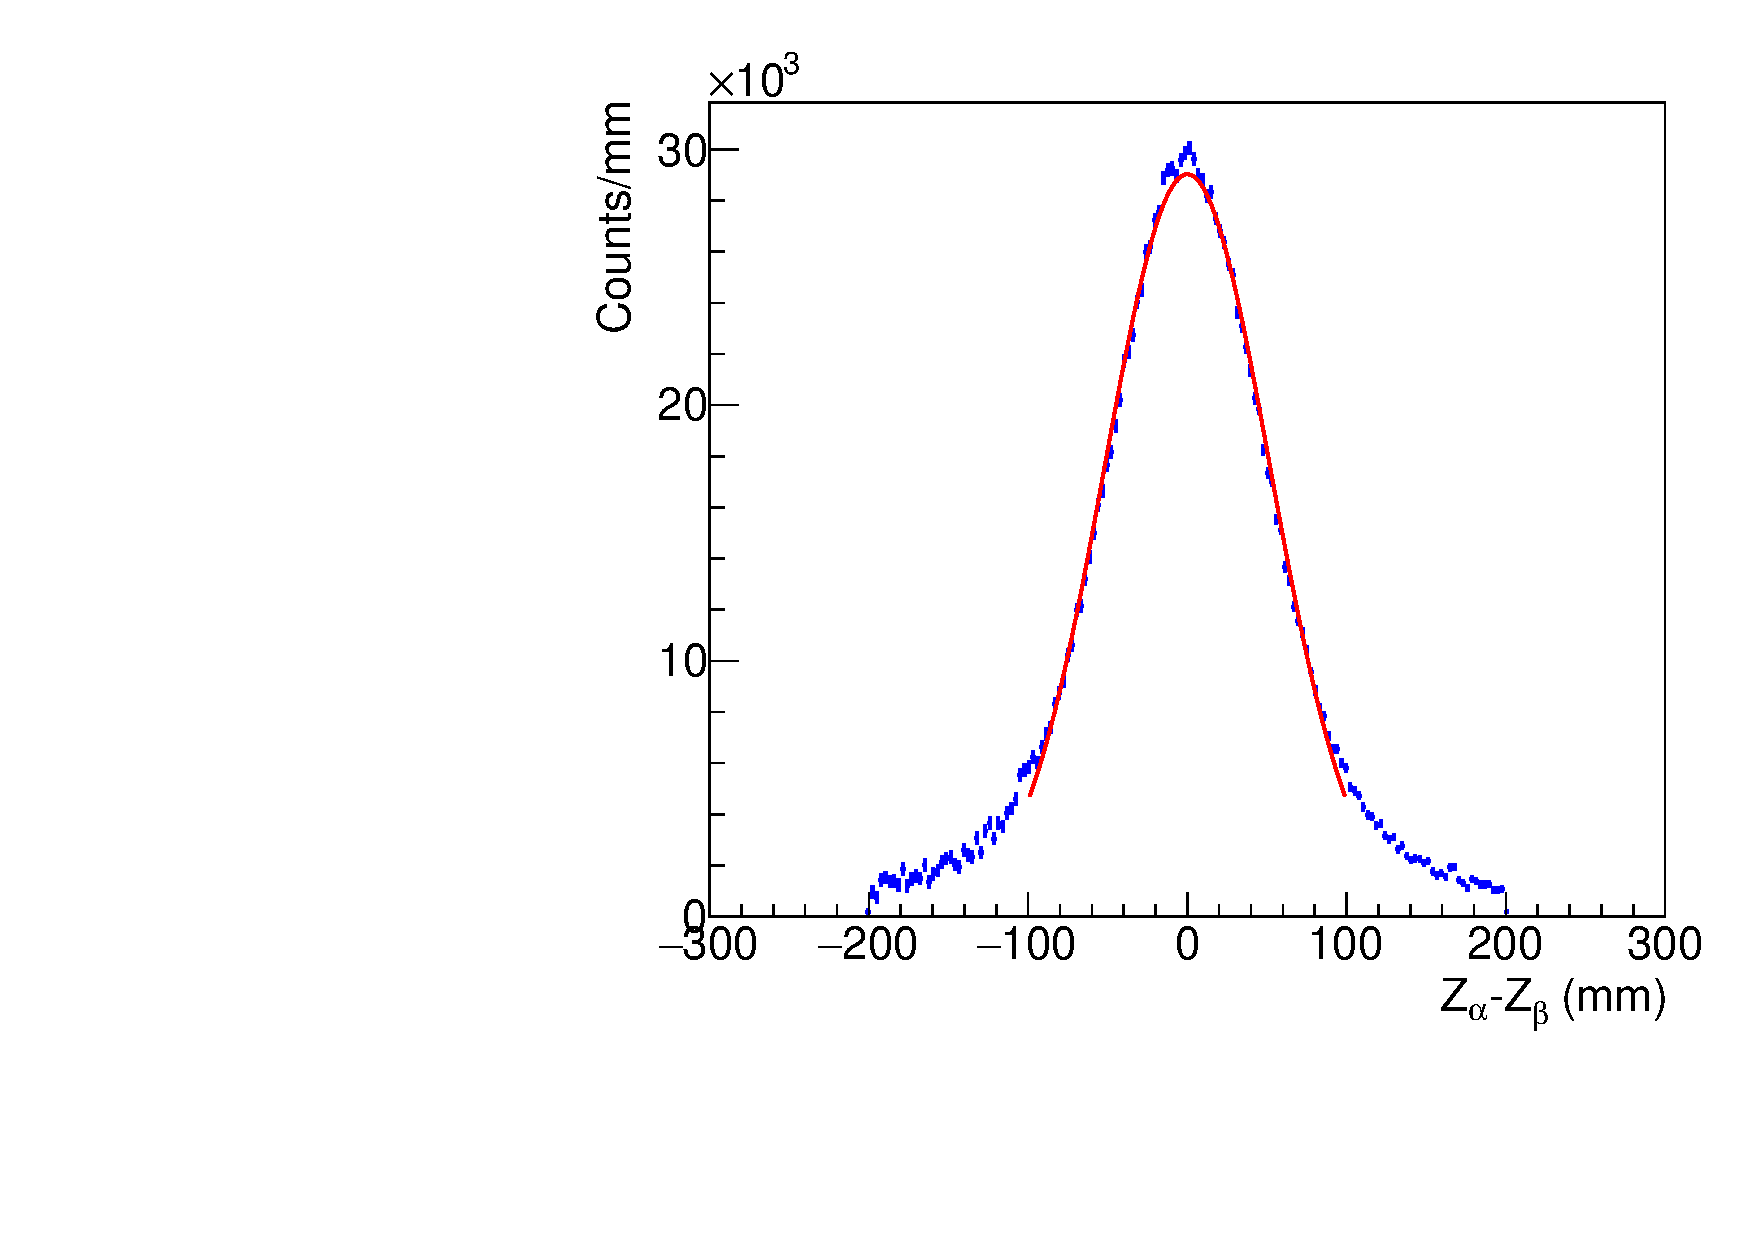
\includegraphics[width=0.6\textwidth]{figures/PubBiPo214dZ.pdf}
\caption{\label{fig:Z214}Whole detector distribution of Po-214 alpha, beta correlation distance $\Delta$Z. The width of this distribution is 52.85$\pm$0.19~mm.}
\end{figure}
\newpage

\FloatBarrier

\section{Supplementary plots\label{sec:supp}}

This section contains supplementary plots that help explain/visualize the analysis process but which are not being submitted for official review for use in publication materials.

\begin{figure}[!h]
\centering
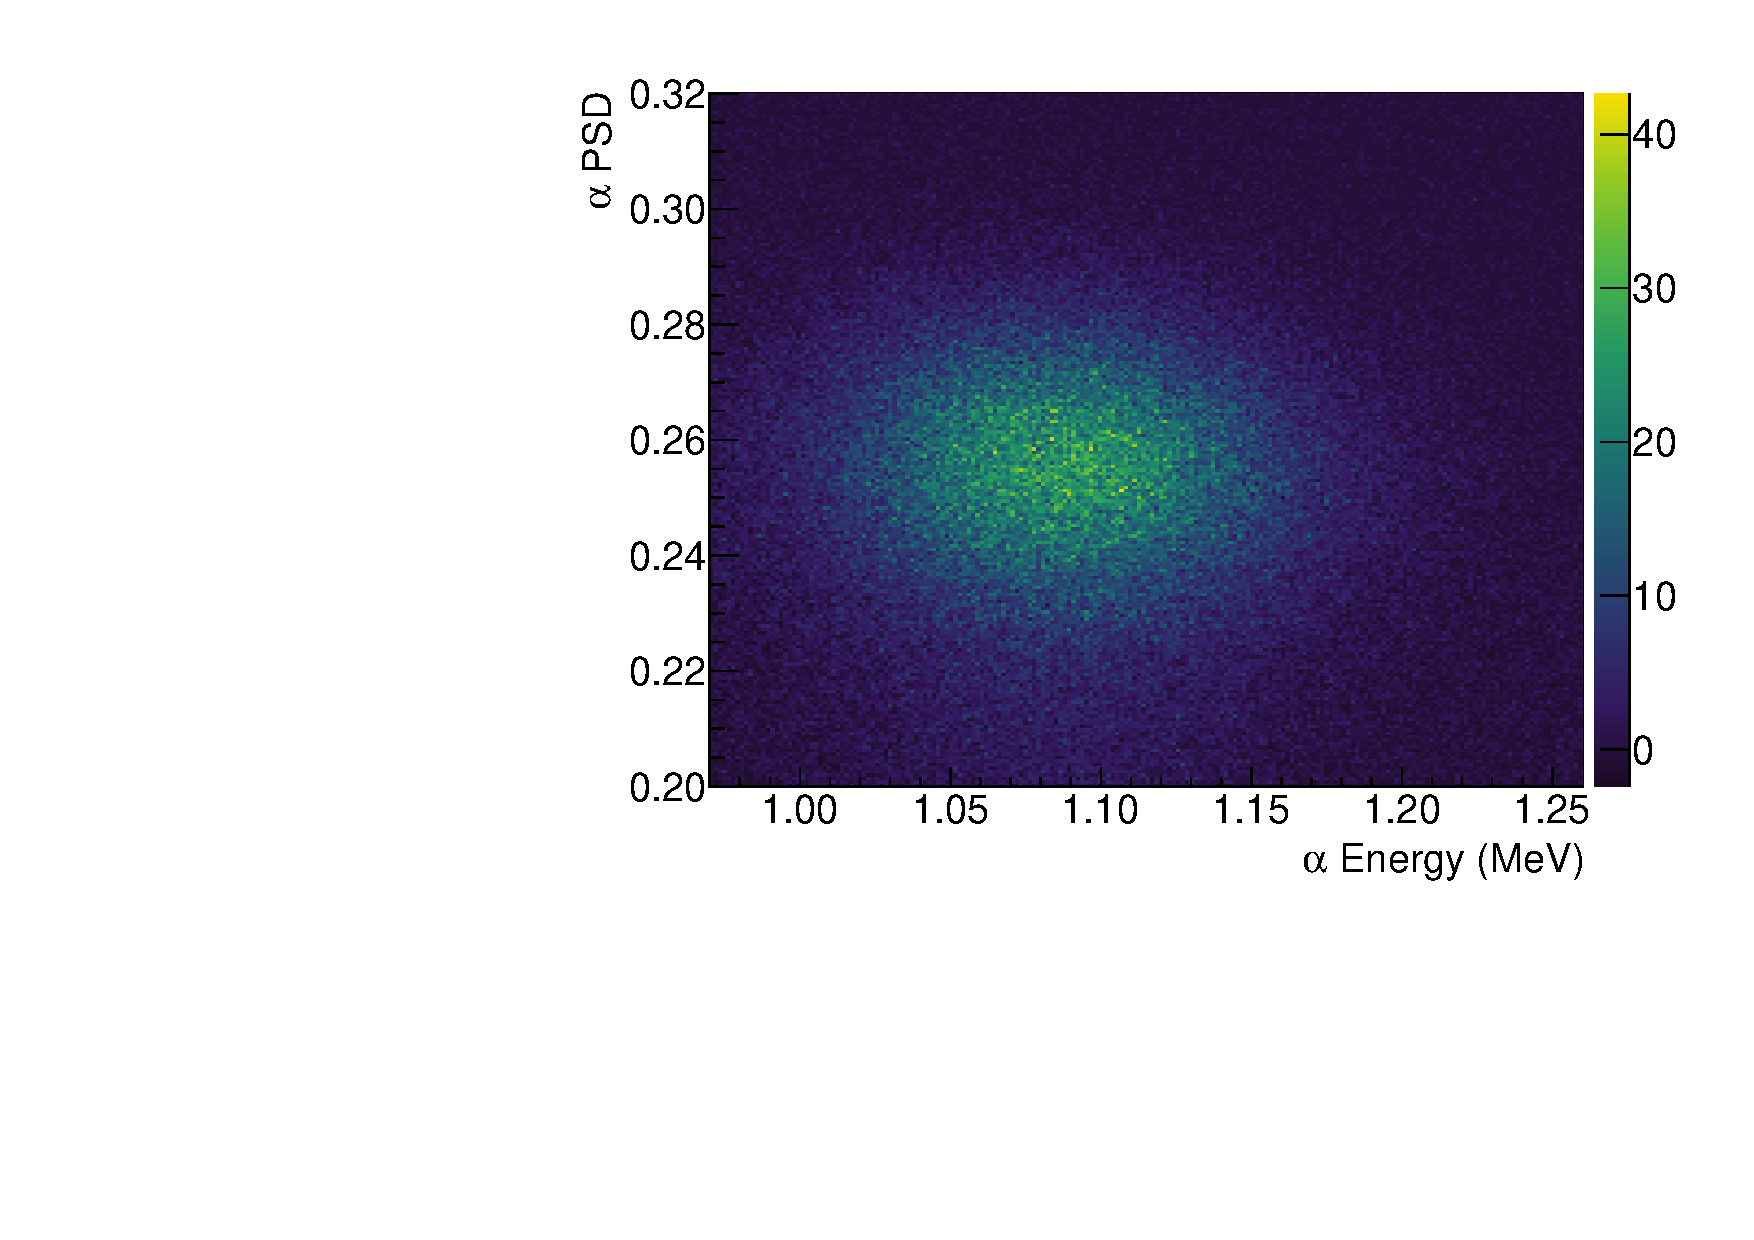
\includegraphics[width=0.7\textwidth]{figures/BiPo212AlphaPSD.pdf}
\caption{\label{fig:apsd212}Po-212 alpha PSD vs energy selection.}
\end{figure}
\begin{figure}[!h]
\centering
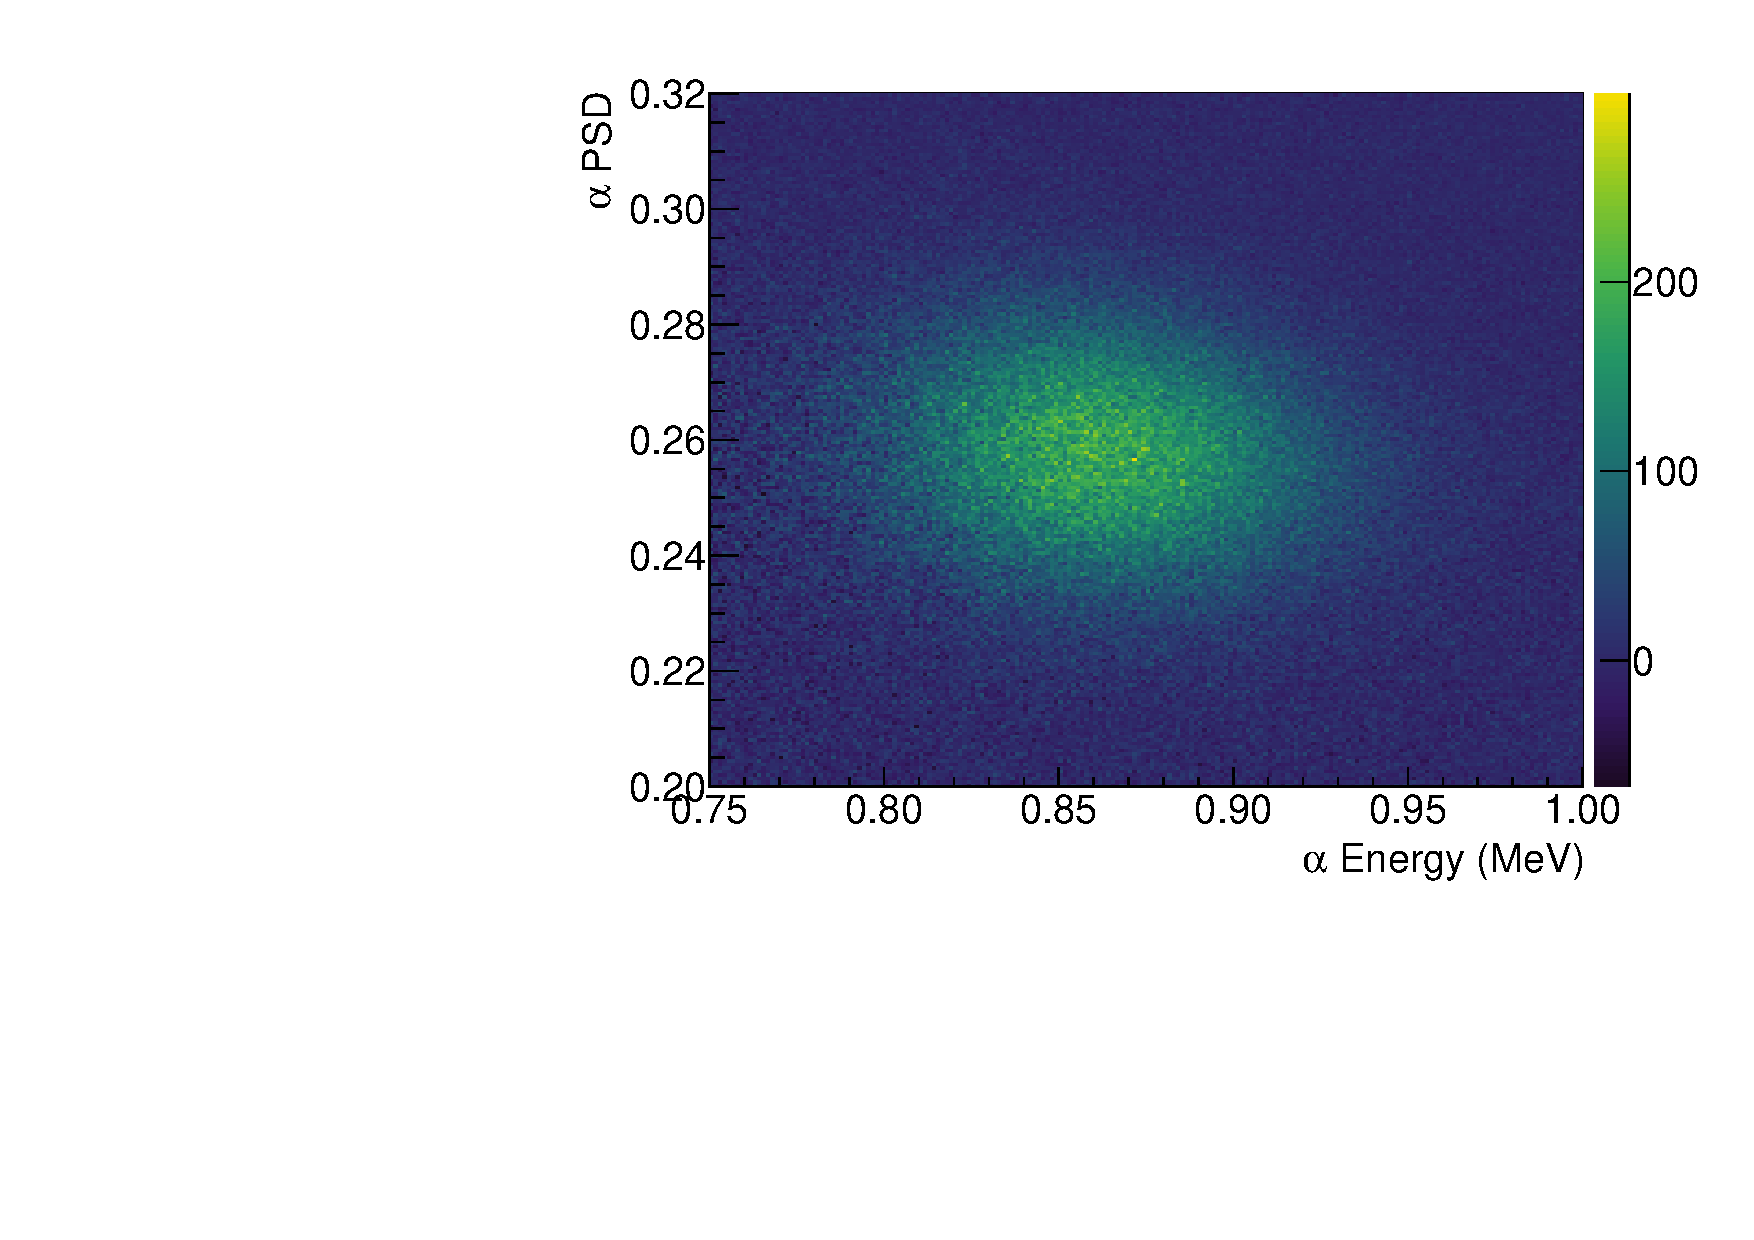
\includegraphics[width=0.7\textwidth]{figures/BiPo214AlphaPSD.pdf}
\caption{\label{fig:apsd214}Po-214 alpha PSD vs energy selection.}
\end{figure}
\begin{figure}[!b]
\centering
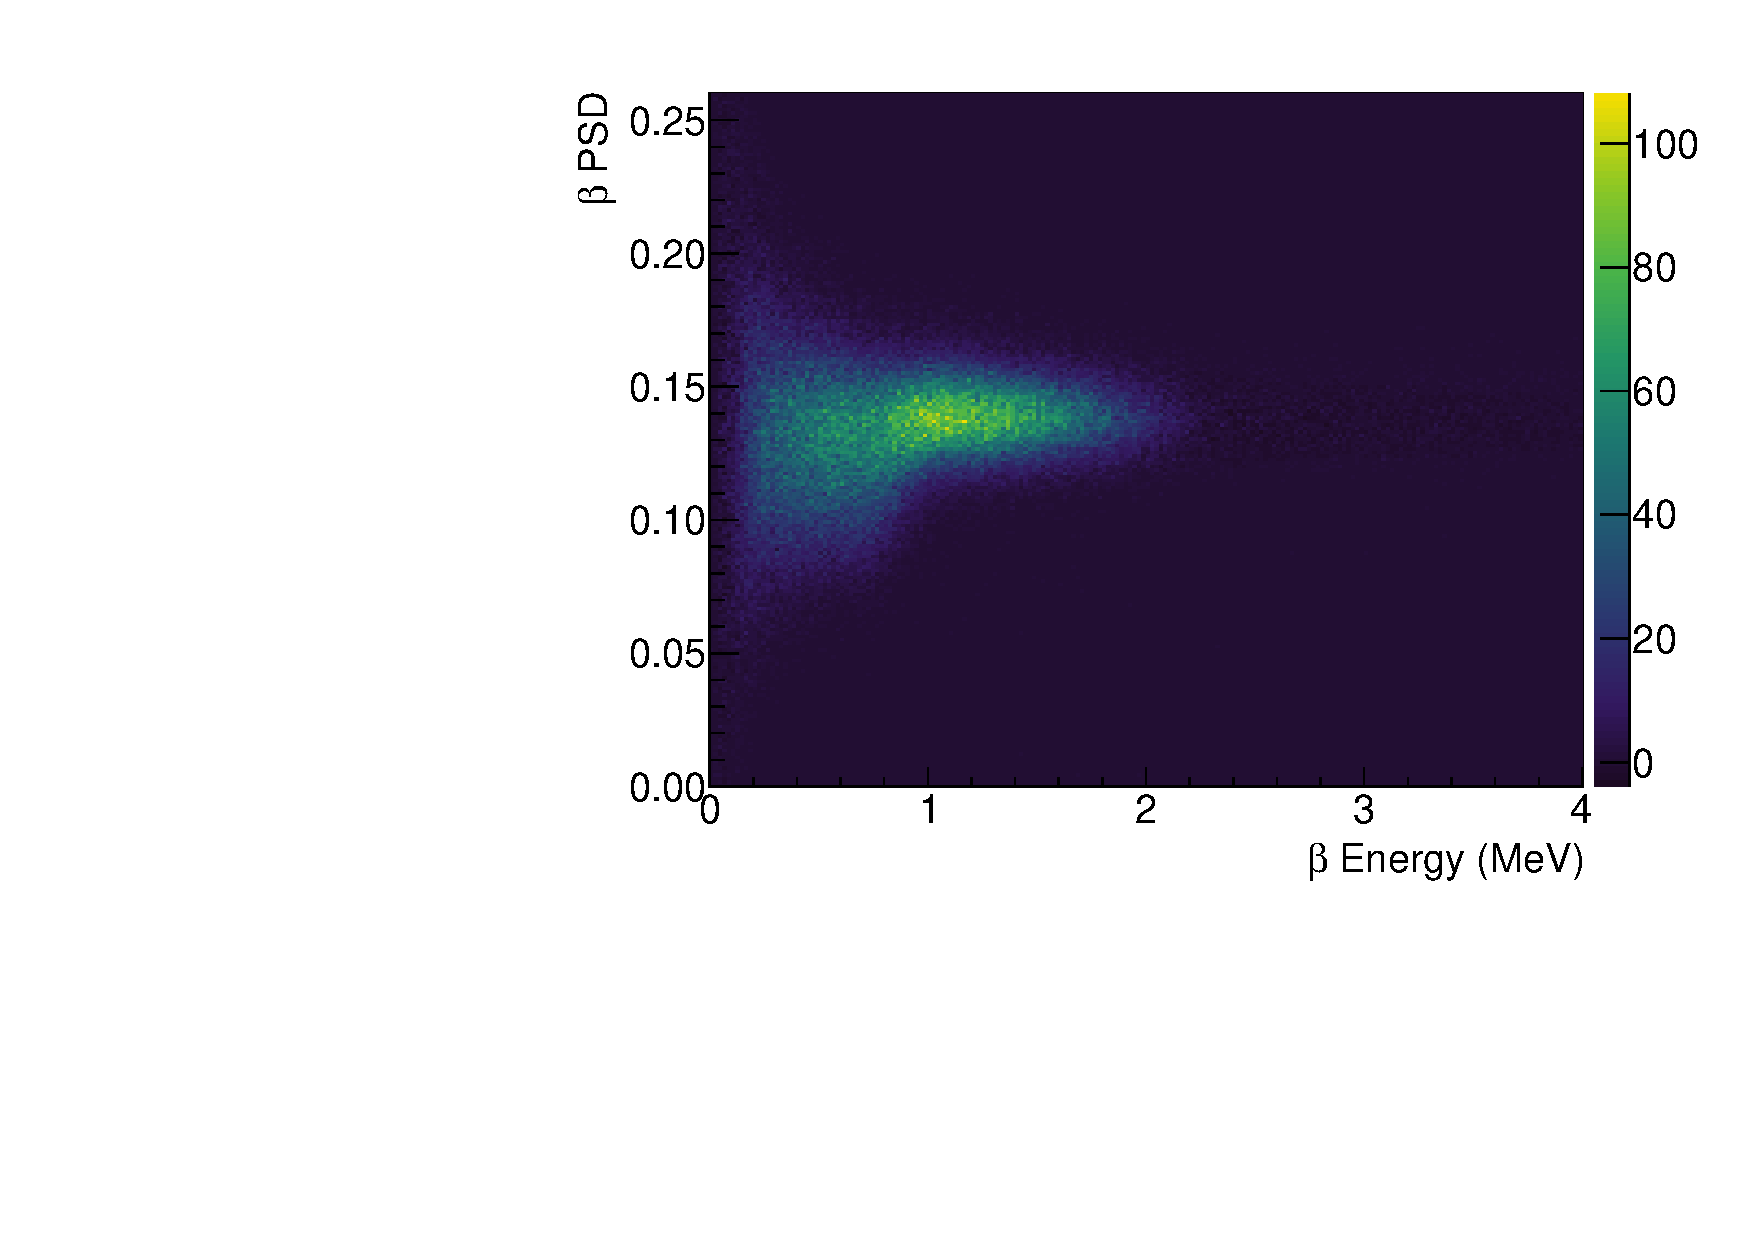
\includegraphics[width=0.7\textwidth]{figures/BiPo212BetaPSD.pdf}
\caption{\label{fig:bpsd212}Po-212 beta PSD vs energy selection. The beta PSD shown here is for the first event in each prompt cluster.}
\end{figure}
\begin{figure}[!b]
\centering
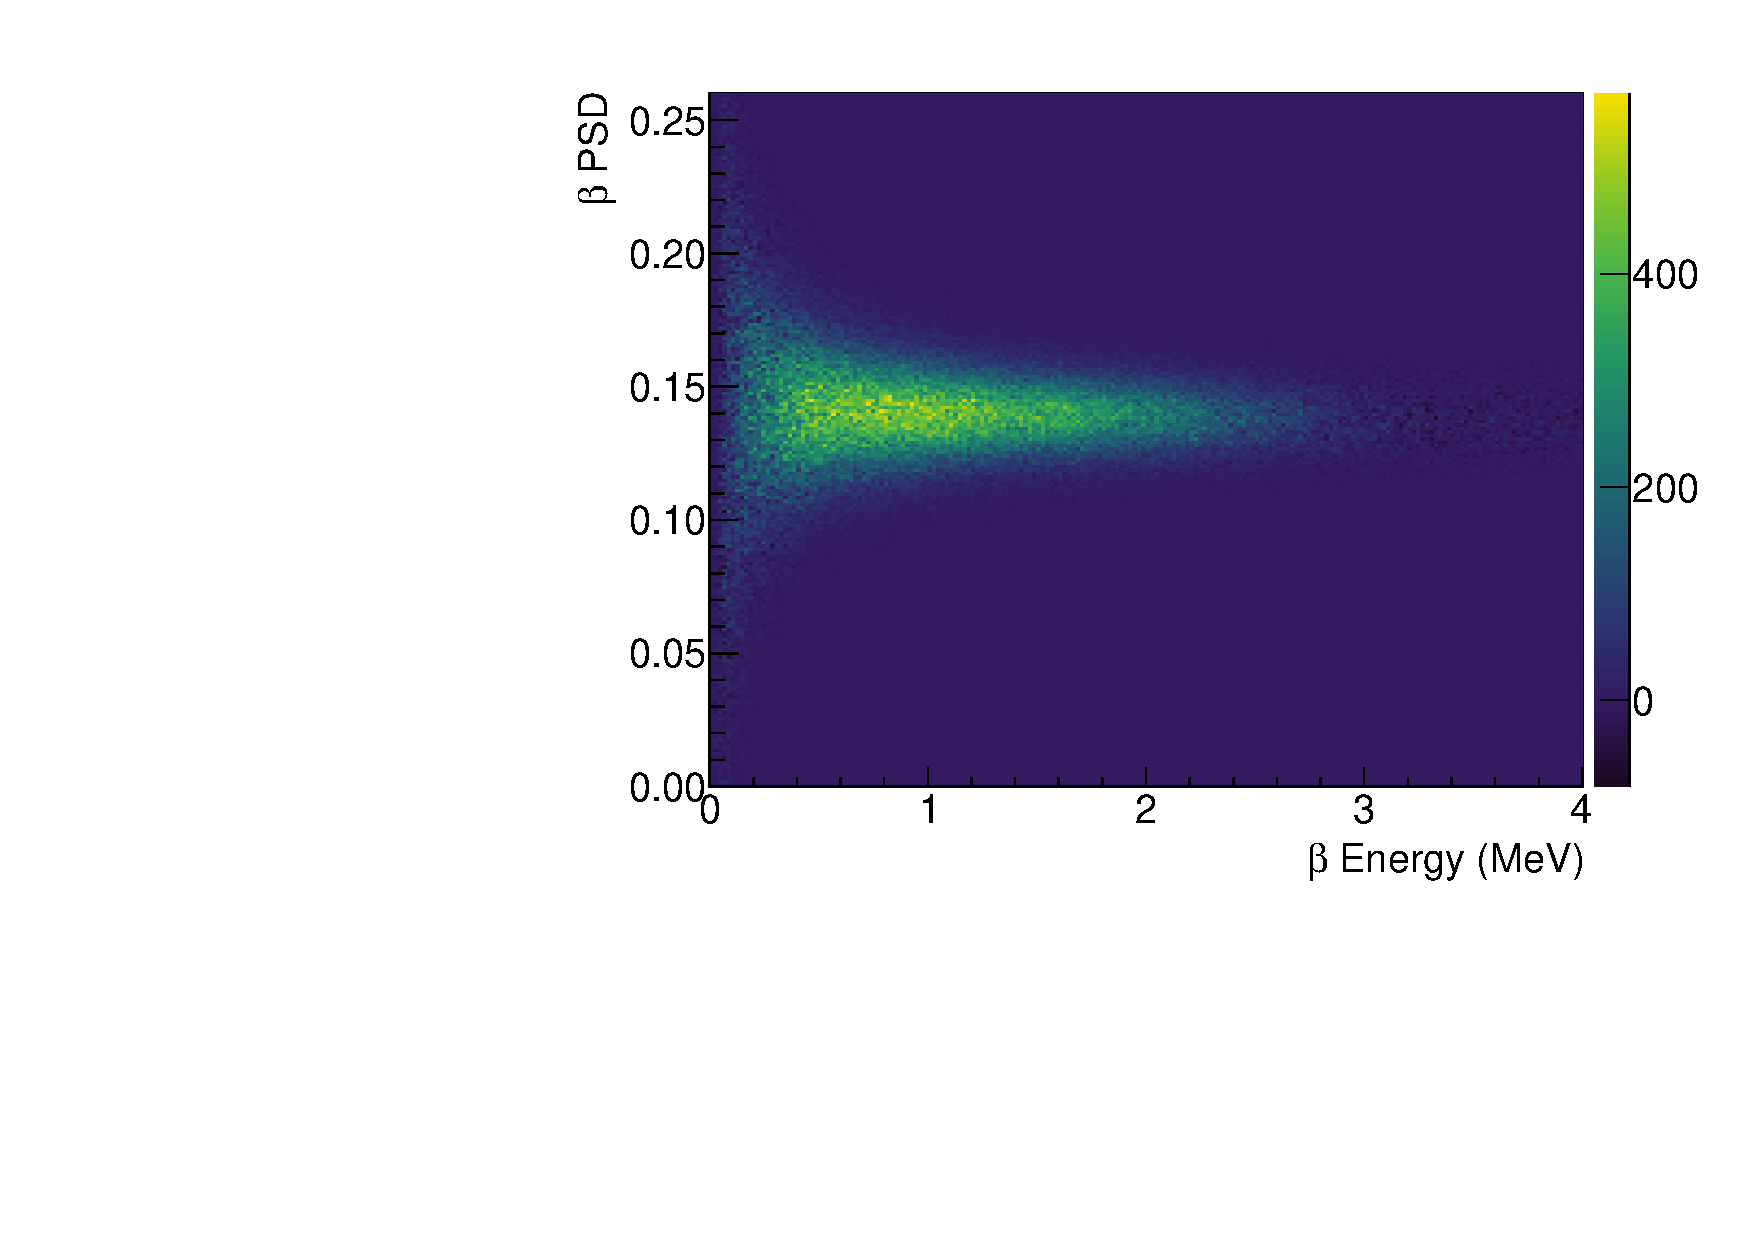
\includegraphics[width=0.7\textwidth]{figures/BiPo214BetaPSD.pdf}
\caption{\label{fig:bpsd214}Po-214 beta PSD vs energy selection. The beta PSD shown here is for the first event in each prompt cluster.}
\end{figure}
\begin{figure}[!b]
\centering
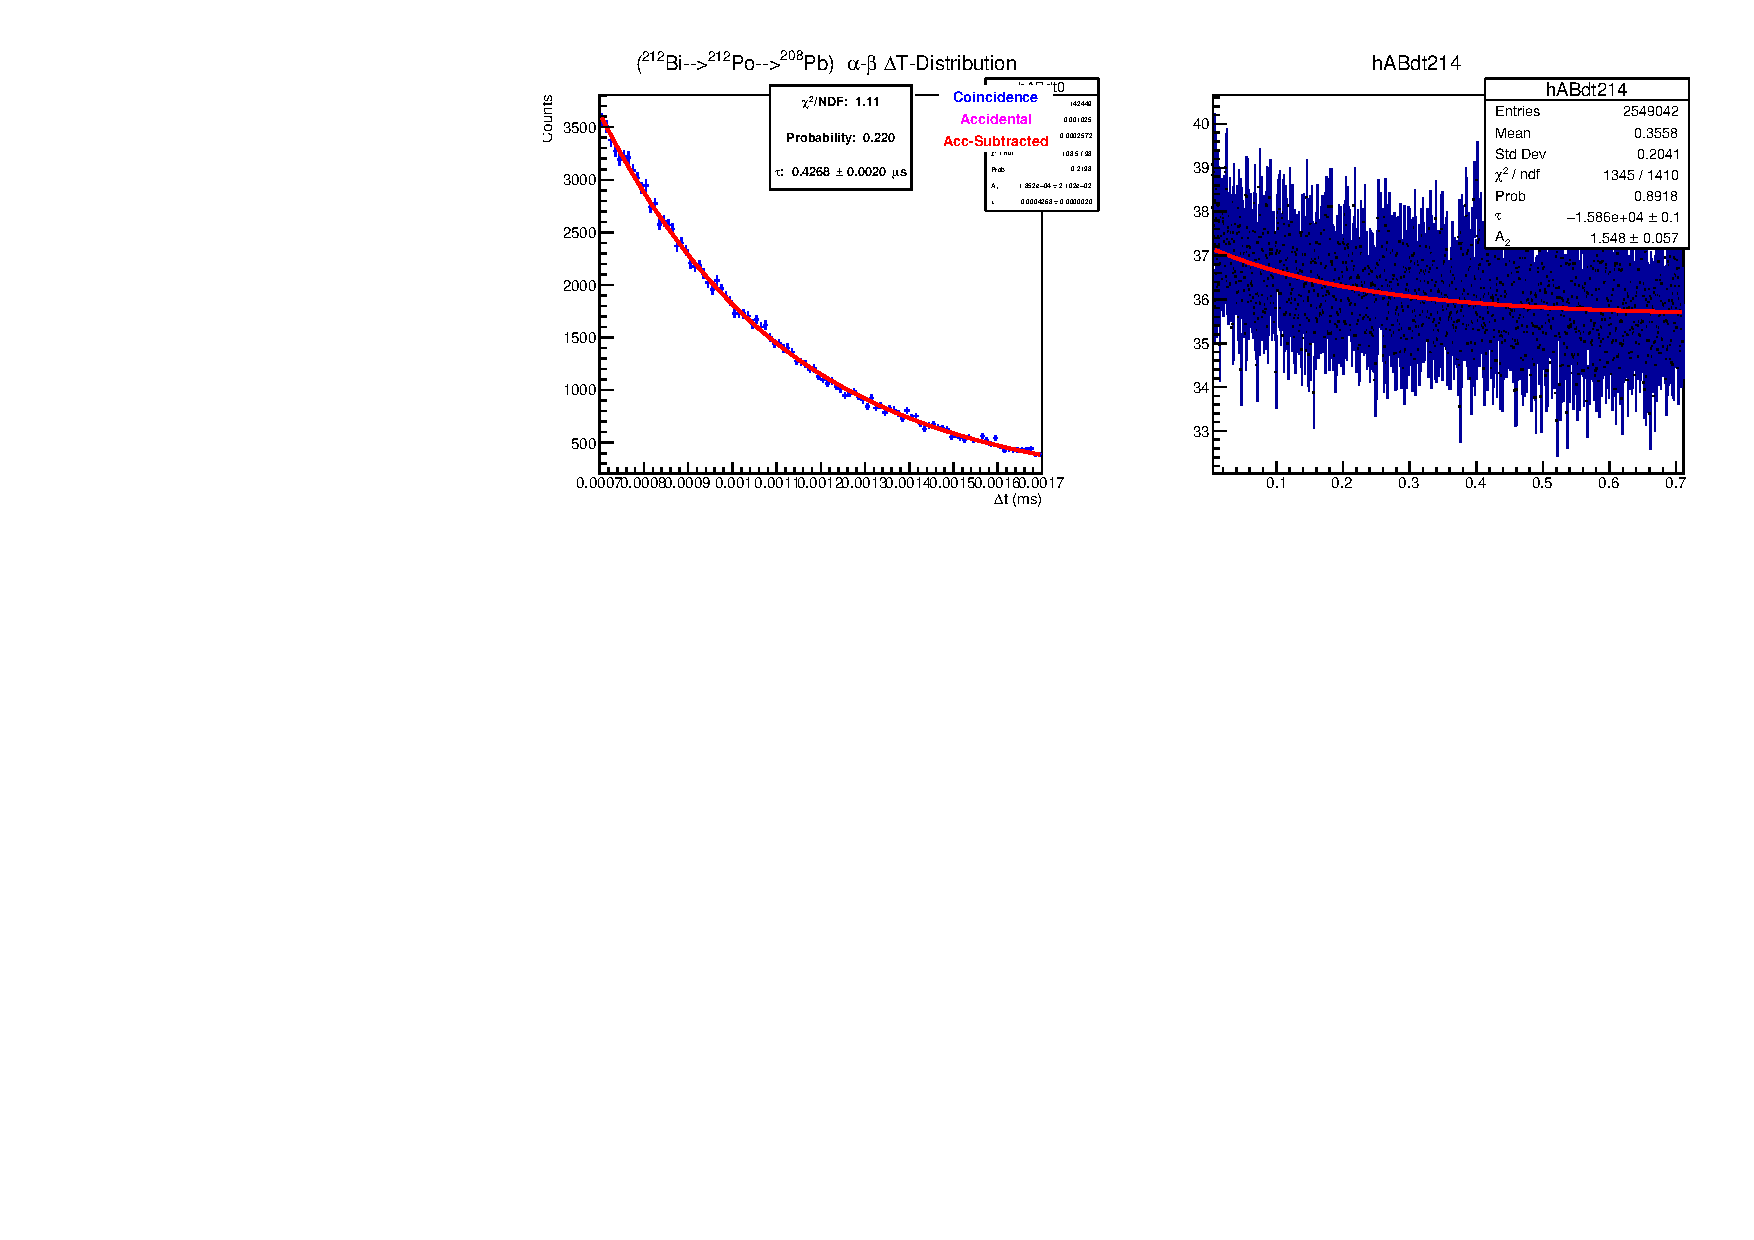
\includegraphics[width=0.7\textwidth]{figures/BiPo212DeltaTSpectrum.pdf}
\caption{\label{fig:dt212}Alpha minus beta time distribution used in Bi-212/Po-212 decay chain analysis. Bins below 0.00066~ms are not used in the fit but are included in analysis. Fit line is extended beyond fit region as a dashed line to demonstrate agreement in smaller dt region. }
\end{figure}

\begin{figure}[!bp]
%\begin{minipage}[b]{0.48\textwidth}
\centering
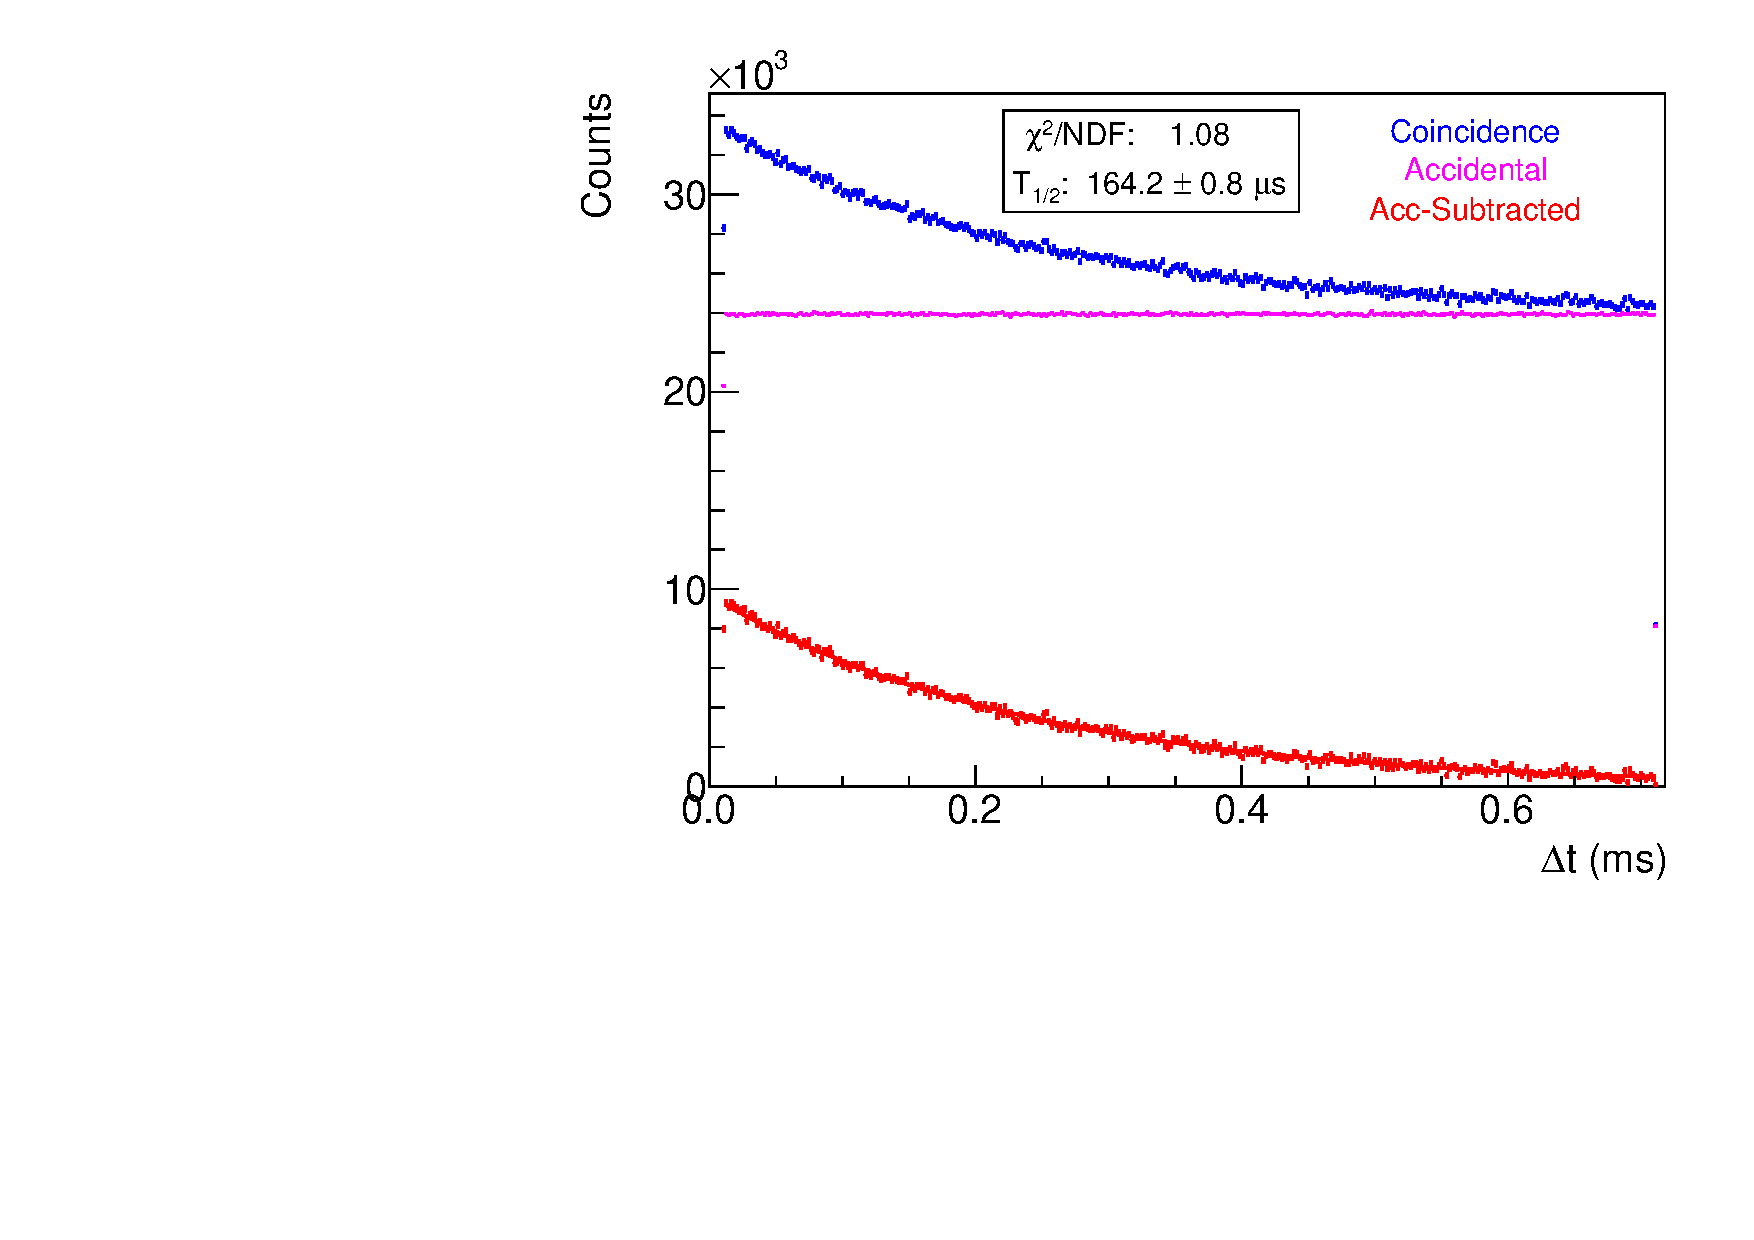
\includegraphics[width=0.7\textwidth]{figures/BiPo214DeltaTSpectrum.pdf}
\caption{\label{fig:dt214}Alpha minus beta time distribution used in Bi-214/Po-214 decay chain analysis.}
\end{figure}
\newpage
\FloatBarrier

\section{Supporting Documentation}

\subsection{Links to any past DocDB entries related to the plot:} 
\hspace{2in}
%\bibliography{}
\bibliography{citations.bib}{}

\end{document}